 \documentclass[11pt,a4paper,english]{memoir}
\usepackage[T1]{fontenc}
\usepackage[latin9]{inputenc}
\setcounter{secnumdepth}{3}
\setcounter{tocdepth}{1}
\usepackage{graphicx}
\usepackage{multirow}


\makeatletter
%%%%%%%%%%%%%%%%%%%%%%%%%%%%%% User specified LaTeX commands.
\usepackage{amsthm}
\usepackage{amsmath}
\newtheorem{definition}{Definition}
\usepackage{a4}
\usepackage{times}
\usepackage{pslatex} 
\usepackage{graphicx}
\let\footruleskip\relax % for compatibility of memoir and fancyhdr
\usepackage{fancyhdr} %\usepackage{fancyheadings}
\usepackage{mscthesis} % determines the used style 
\usepackage{lipsum} % standard filler text, only needed for demo
\usepackage{url}
\usepackage[ruled]{algorithm2e}
\usepackage{algpseudocode}

% Include right (LaTeX/PDFLaTeX) graphics package
% (doesn't work under cygwin apperently)
%\ifx\pdftexversion\undefined

\@ifundefined{definecolor}
 {\usepackage{color}}{}

%\else
%\usepackage[pdftex]{graphicx}
%\usepackage[pdftex]{color}
%\fi

%---------------------------------------------------------------------%
%                     Options                                         %    
%---------------------------------------------------------------------%

\title{Distributed Regular Path Query Matching and Optimization for Graph Database
based on Spark
} % CHANGE TO YOUR TITLE
\subtitle{1\today} 

% The final version of your thesis should typically use a different
% subtitle without the current date, for example \subtitle{Master's Thesis} 
% overwrite the subtitle by using the following line: 

\subtitle{Master's Thesis}

\university{
\hskip-10pt
{

\includegraphics[height=2cm]{img/TU_Delft_Logo.pdf}
}\\
[-8pt]
Web Information Systems \\
Department of Software Technology \\
Faculty EEMCS, Delft University of Technology \\
Delft, the Netherlands \\
\url{http://wis.ewi.tudelft.nl}
}


\author{Canran Gou} % CHANGE TO YOUR NAME
\birthplace{GUIZHOU} % CHANGE TO YOUR BIRTHPLACE
\studentid{4312805} % CHANGE TO YOUR STUDENT ID
\authoremail{\url{canrangou@email.com}} % CHANGE TO YOUR EMAIL ADDRESS

% Optional for work done at a company, put this in comments if you did
% not do your thesis work at a company
%\company{
%\includegraphics[height=2cm]{img/hilbert.ps}\\
%Some Company\\
%With it's address\\
%ThePlace, the Netherlands\\
%\url{www.url.nl}
%}
% Optional (postscript) cover picture. Put this in comments when not needed.
%\coverpicture{\includegraphics[width=11cm]{img/pyramid.eps}}


% A copyright notice and maybe something about the cover picture
% Put in comments to get the default copyright notice
\colophon{\noindent\copyright{} \the\year~\theauthor. Coverpicture: some picture.}

% thesis committee:
\chair{Prof. dr. ir. G.J.P.M.Houben, Faculty EEMCS, TUDelft}
\supervisor{Dr. ir. A.J.H.Hidders, Faculty EEMCS, TUDelft}

% The following two are optional for LaTeX (current university regulations state that at least one of them should be assigned)

\committeemember{Dr. ir. A.L.Varbanescu, Faculty EEMCS, TUDelft}
%\externalsupervisor{Ir. H.J.A.M. Geers, Faculty EEMCS, TUDelft}


\setsecnumdepth{subsection}\maxsecnumdepth{subsection}

\makeatother

\usepackage{babel}

\begin{document}
\frontmatter 

\thispagestyle{empty}

\maketitle % main title page

\makeformaltitlepages{We live in a world of connections where everything shares relationships like follow/subscribe in Social Network or protein interactions in Biology Network. A Graph database embraces relationships and supports low-level join as its nature. Regular Path queries (RPQs) are queries run against graph database, which are written in form of regular expressions based on edge labels and with strong flexibility and expressiveness.

Unlike some graph databases where actual data stored
and queried using standard relational mechanisms, in this thesis we investigate three distributed algorithms by storing graphs with NoSQL data model and evaluating RPQs with Apache Spark.

The three algorithms are cascaded 2-way join, multi-way join and Dan Suciu's Algorithm. The performance of them regarding to running time and network communication volume are compared, and main bottlenecks are identified. Dan Suciu's algorithm shuffles the least data during evaluation, meanwhile the performance is heavily influenced by the ways of partitioning the graphs. In theory we found that the size of GAG (Global Accessible Graph) collected to driver-side, which affects communication volume and computation scale on driver-side, is related to the number of input-nodes in distributed graph. 

So in this thesis project we also try to optimize the execution of Dan Suciu's algorithm with various partition strategies such as METIS or JabeJa. Based on JabeJa, which tries to minimize the number of cross-edges, we propose a distributed algorithm JabeJa* to minimize the number of input-nodes in graph. In the best cases, those strategies can reduce the communication volume to 30\%, driver-side compuation time to 30\% and overall running time to 50\%.

} % formal title pages

\cleardoublepage{}
\chapter{\label{cha:Preface}Preface}
###########################
It has been a thrilling journey since I started working on this thesis project. Although graph databases and regular path queries have already been studied since more than 20 years ago, combining them with latest technologies such as Apache Spark and Cassandra/HBase is still such a fresh and innovative experience for me. Besides, by following the development of the latest tools such as Titan, I came to understand why and how those projects can change the play in the big data world and real world.

First of all, I'd like to express gratitude for my supervisor dr.ir. Jan Hidders, who can always give the most helpful suggestions in a timely manner to keep the project forward, despite the fact that my 'stupid' ideas or grammar errors are coming up sometimes. At the same time, thanks to professor dr.ir. Geert Jan Houben and dr.ir. Ana Lucia Varbanescu for spending their precious time on reading my thesis and giving valuable feedback.

I want to give special thanks to Mr. Jeroen Schot from Surf Sara, who kept fighting against the bugs of Spark on Hbase and
 made my application run successfully on their cluster. Without his effort, Chapter 7 and 8 would only have some simple results from the expensive Google Cloud platform.
 
I am especially grateful to my parents and my girlfriend, who gave me both financial and spiritual support in the past years and finally helped me getting closer and closer to the master degree.

The guys in Alpha group, you are awesome and I can't be more lucky to work around you during the thesis project. Hope you are well and good luck with your future research.

\vskip1cm 

\begin{flushright}
\theauthor\\
 Delft, the Netherlands \\
 \today\\
 
\par\end{flushright}


\cleardoublepage{}\tableofcontents{}\cleardoublepage{}\listoffigures
\cleardoublepage{}

\mainmatter


\chapter{\label{cha:intro}Introduction}

As social networks are gaining more popularity today, the graph model is found to be a natural data model in numerous areas. For example, Figure \ref{fig:new-example} models a researcher network, in which nodes represent entities such as professors, papers, universities, etc., and edges are diverse relationships between them.
\\A graph database is a database that uses graph structures with nodes, edges and properties to store and query data. One problem of existing graph databases is that none of them support distributed storage and distributed evaluation of regular path query (RPQ) at the same time. So in this project, we investigate distributed algorithms on Apache HBase/Cassandra (Distributed Storage) and Apache Spark (Distributed Computation) to evaluate regular path query.

\begin{figure}[h!]
  \caption{Example - Researcher Network}
  \label{fig:new-example}
  \centering
    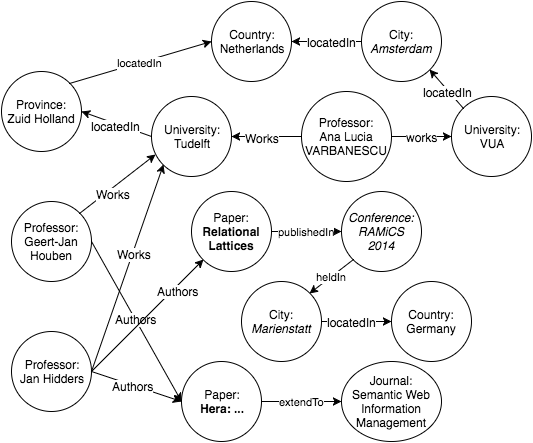
\includegraphics[width=0.5\textwidth]{img/new-example}
\end{figure}

A regular path query (RPQ) consists of node variables $X,Y$ and regular expression $R$ in the form of $(X,R,Y)$. The result should be pairs of nodes $(x,y)$ where there exists a path between them that the edge-label sequence of the edges satisfying $R$. For example, we can run several RPQs for Research Network in Figure \ref{fig:new-example}:
\begin{enumerate}
    \item $(X,authors*author^-,Y)$: Finding two professors who co-author a same paper. In this network, the result will be pairs (Jan Hidders, Geert-Jan Houben) and (Geert-Jan Houben, Jan Hidders), since there are paths between the nodes representing those two professors that satisfy the regular expression.
    \item $(X,works*locatedIn^*,Y)$: Finding all places where the professors work in, the result can be (Ana, VUA), (Ana, Zuid Holland), (Jan Hidders, Netherlands), etc. Here we introduce kleene star since the locations can be at different levels( university, city or country ).
    \item $(X,author*(publishedIn|extendTo))$: This query will return the pairs of professor and conference/journal.
\end{enumerate}
The usual way to evaluate RPQ is cascaded two-way join, multi-way join\cite{afrati2010optimizing}, and Dan Suciu proposed a distributed architecture/algorithm for RPQ evaluation\cite{suciu2002distributed}. In distributed computation context, network communication is usually a crucial overhead/bottleneck during computation. One observation of the experiments about Dan Suciu's algorithm is that different partition configurations for graphs will influence the size of data transmitted on the network. In this project, we will explore different properties of partition strategies for distributed graphs and their influence on communication cost for distributed RPQ evaluation algorithms.

\section{Research Questions}
The main goals of this thesis work can be divided into two parts, and they can be split into following sub-questions:
\begin{enumerate}
\item How to solve regular path queries and conjunctive regular path queries in parallel with Apache Spark?
    \begin{enumerate}
    % \item How to translate regular path queries into data structures we can evaluate with?
    \item What data model should be used for graph storage to evaluate regular path queries efficiently?
    \item How to implement distributed algorithms for efficient query evaluation with Apache Spark?
    \item What's the pros and cons for different algorithms?
    \end{enumerate}
\item How could different partition strategies optimize the querying performance?
\begin{enumerate}
    \item What is the crucial factors leading to the bottleneck? 
    \item How to improve those factors with different partitioning strategies in order to optimize the querying performance?
\end{enumerate}
% \item How to optimize the query performance for CRPQ with vertex signature tree (VS-tree) ?
%     \begin{enumerate}
%         \item How to use VS-tree to speedup query performance?
%         \item What's the trade-off between index size and speedup?
%     \end{enumerate}
\end{enumerate}

\section{Approach}
Firstly I will look for edge-labelled graph data-sets as the benchmark, and those containing data and queries at the same time or with various labels will be preferred. Secondly, the system which consists of Spark and Cassandra/HBase will be deployed. A suitable data model will be selected to store benchmark graphs. When coming to implementation, experiments will be conducted with different algorithms and increasing number of workers for RPQ. For Dan Suciu's algorithm, different partitioning strategies will be examined with regards to different graph properties, running time and network communication of applications.

\section{Outline}
In Chapter 2 we will explore the research background briefly, including existing graph databases, regular path queries and related algorithms. Chapter 3 presents the basic data model, system architecture and the benchmarks. In Chapter 4-6 we will focus on introducing and giving the execution process in Spark for different distributed algorithms. After that, those algorithms will be evaluated and compared in Chapter 7. In chapter 8 we investigate the reason different partition strategies affect performance and develop a new distributed partition strategy to minimize the number of $input-nodes$. Finally we will give conclusion in Chapter 9. 
\chapter{\label{cha:res-bg}Research Background}

\section{Edge Labelled Graph}
A graph $G$ can be modelled as a pair $(V, E)$, where $V$ is a finite set of nodes and $E$ is a finite set of edges connecting pairs of nodes. In some cases, the edges are labelled with strings from a finite set of symbols, representing the attribute value from starting node to ending node. The symbols are drawn from some finite alphabet $\Sigma$; Hence a labelled directed graph could be modelled as 
$(V,E,\Sigma)$, where $E\subseteq V\times\Sigma\times V$.\\
\section{Graph Database}
In the context of graph databases, we focus on permanent storage and query evaluation at the same time, which is why graph processing framework such as Pregel or Trinity are not taken into consideration here.
\subsection{Vertical Scaling Graph Database}
\textbf{Neo4j}\cite{neo4j} is one of the most popular graph databases, which provides full ACID transaction support, indexing, a web UI for graph visualisation and supports diverse query languages such as Cypher, Gremlin and even SPARQL. Neo4j uses a custom disk-based native storage engine. Neo4j believes vertical scaling could solve most scaling problems of graph databases, so Neo4j graph database can only be deployed on a single machine. With Cypher, we can query Neo4j with a subset of RPQ and write queries like this: MATCH $ n-[?:KNOWS*..5]->m$, which will find out all pairs $(n,m)$ where there are paths between them consisting of at most 5 "KNOWS" labels.\\

\noindent\textbf{Sparksee}\cite{sparksee} is a graph database written in C++ and provides API in diverse programming languages in Python, C++, .Net, Java, Objective-C, etc. It can be deployed on Linux, Windows, MacOSX and even mobile systems such as Android or IOS. Sparksee splits graphs into small structures and caches the most significant parts. It also has mechanisms for indexing nodes, edges and attributes. It supports concurrent query processing, but not distributed storage and querying.

\subsection{Distributed Graph Database}

\textbf{Titan}\cite{titan} is one of the most popular distributed graph databases, which can use different storage back-ends such as Cassandra, HBase or BerkeleyDB. Although Titan 1.0 released in September, 2015 has implemented the latest version of the popular Apache Gremlin query language, from which it's possible to traverse graphs by the Spark-gremlin connector in a distributed way, the project is still far from maturity and under community testing. Furthermore, graph analytics and global breadth-first execution of Gremlin queries is executed by Apache Spark through the Cassandra-Spark connector, which is similar to our own system architecture.\\


\noindent\textbf{imGraph}\cite{imgraph} is a distributed in-memory graph database, which provides distributed memory storage and distributed processing features, however, it doesn't support regular path queries and huge graphs cannot always fit in memory.\\

\noindent\textbf{OrientDB}\cite{orientdb} is a database of hybrid Document-Graph data models. In order to achieve higher scalability, it adopts Multi-Master + Sharded architecture: all the servers are masters. Similar to Neo4j, OrientDB has its own query language OrientDB SQL, which is quite similar to SQL syntactically.\\

\noindent\textbf{GBase}\cite{GBase} is a platform conceived to handle large static graphs that uses the sparse adjacency matrix format as data model. The graph data is stored and indexed by storing compressed blocks in distributed storage such as HDFS. It does not support RPQ and cannot work for dynamic graphs.\\

\noindent\textbf{Infinitegraph}\cite{infinitegraph} is an enterprise distributed graph database implemented in Java. In its graph data model, edge is the first-class entity with an identity independent of the vertices it connects. Infinitegraph supports full ACID, and provides path pattern matching feature.\\

To summarize, I extend the table which compares graph databases in imgraph paper\cite{imgraph} to following table 2.1.
\begin{table}[h!]
\scriptsize
\def\arraystretch{1.5}
\centering
\caption{Graph Database Overview}
\label{graph-database-overview}
\begin{tabular}{|l|m{5em}|m{5em}|m{5em}|m{5em}|m{5em}|m{5em}|}
\hline
 & Native Graph Model & Distributed Storage & Distributed query processing & Transactions and index support & Support RPQ & License \\
\hline
Neo4j & Yes & No & No & Yes & Partially & Conditional \\
\hline
Sparksee & Yes & NO & NO & Yes & No & Free Research License \\
\hline
Titan & Yes & Yes & No & Yes & No & Free \\
\hline
imGraph & Yes & Yes & Yes & Yes & No & Free \\
\hline
OrientDB & Yes & Yes & Yes & Yes & No & Conditional \\
\hline
GBase & No & Yes & Yes & No & No & Free \\
\hline
Infinitegraph & Yes & Yes & Yes & Yes & No & Enterprise\\
\hline
\end{tabular}
\end{table}
\section{Regular Path Query Classes}
There are a variety of ways to define the classes for RPQ. For example, in Wood's work\cite{wood2012query}, RPQs are divided into four classes:
\begin{enumerate}
\item conjunctive queries (CQ)
\item regular path queries (RPQ)
\item conjunctive regular path queries (CRPQ), which is the combination of CQ and RPQ.
\item extended conjunctive regular path queries (ECRPQ).
\end{enumerate}
In the paper by Reutter et al. \cite{reutter2015regular}, he and his colleagues extend the expressiveness of RPQ. More categories are produced:
\begin{enumerate}
\item 2-way regular path queries (2RPQ), in which inverse labels are allowed.
\item conjunctive two-way regular path queries (C2RPQ)
\item nested two-way regular path queries (N2RPQ), where recursive variable is allowed in regular expression.
\item union of conjunctive two-way regular path queries (UC2RPQ), where we can perform unions, joins and projections over 2RPQs.
\item union of conjunctive nested two-way regular path queries (UCN2RPQ), where we can perform unions, joins and projections over N2RPQs. 
\end{enumerate}
In this thesis work, the query classes can be reduced by allowing inverse edges and nested variables in regular path query. For conjunctive regular path queries, we will stop at C2RPQ, which means calculating the intersection of results of 2RPQs.
\subsection{Regular Path Query}
Given a finite alphabet $\Sigma$, the regular expression over $\Sigma$ is defined by following grammar:
$$ n := \ \epsilon \ | \ a \ (a\in \Sigma) \ | \ a^- \ (a\in \Sigma) \ | \ n\ + \ n \ | \ n\ *\ n \ | \ n^* \  $$
The regular expression $n$ can be one of the following:
\begin{enumerate}
    \item Empty Expression.
    \item A label $a$ from $\Sigma$.
    \item The reverse of a label $a$ from $\Sigma$.
    \item The alternation of two regular expressions.
    \item The concatenation of two regular expressions.
    \item Zero or more recurrence of a regular expression.
\end{enumerate}
Furthermore, The semantic of regular path expression over a graph database $G=(V,E)$ can be defined as binary relation $[n]_G$ as follows:
$$[\epsilon]_G = \{(u,u) \ |u\in V\}$$
$$[a]_G = \{(u,v) \ |\ (u,a,v) \in E\}$$
$$[a^-]_G = \{ (u,v) \ |\ (v,a,u) \in E\}$$
$$[n_1\ +\ n_2]_G = [n_1]_G \ \cup \ [n_2]_G $$
$$[n_1\ *\ n_2]_G = [n_1]_G \ \circ \ [n_2]_G$$
$$[n^*]_G = [\epsilon]_G \ \cup \ [n]_G \ \cup \ [n*n]_G \ \cup \ [n*n*n]_G \ \cup \ ...   $$
where $[n_1]_G \ \circ \ [n_2]_G=\{ (u,v) | \ \exists w \ such \ that \ (u,w)\in [n_1]_G \ and \ (w,v) \in [n_2]_G \}$. By convention, we treat $[n^+]_G$ as $[n]_G*[n^*]_G.$
\subsection{Conjunctive Regular Path Query}
\subsubsection{Conjunctive Query}
For a set of node variables $\{ x_1,y_1,x_2,y_2,...,x_m,y_m \}$, the conjunctive query(CQ) Q over a finite alphabet $\Sigma$ is a query in the form:
$$ans(z_1,z_2,...,z_n) \leftarrow \cap_{i=1}^{m} (x_i,a_i,y_i)$$
where $m>0$, each $a_i \in \Sigma (1\leq i \leq m)$ and each $z_i$ is some $x_j$ or $y_j$ $(1\leq i \leq n,1\leq i \leq m)$. The semantics of CQs of this form is finding all node binding for all node variables in a graph. For example, a CQ for MATRIX graph could be:\\
$$ans(x,y)\leftarrow (x,LOVES,y),(x,KNOWS,y)$$
which return (Neo,Trinity) as it's the only pair that satisfies the node bindings for x and y.\\
The CQs are in some sense the simplest form of graph queries, the complexity of which is NP-complete as it's the same as the problem of subgraph homomorphism.
\subsubsection{Conjunctive Regular Path Query}
Conjunctive Regular Path Queries are similar to Conjunctive Query, except replacing symbol $a_i$ with a regular expression $r_i$. So a conjunctive regular path query(CRPQ) Q over $\Sigma$ is an expression of the form:
$$ans(z_1,z_2,...,z_n) \leftarrow \cap_{i=1}^{m} (x_i,r_i,y_i)$$
The example in previous section then could be:
$$ans(x,y)\leftarrow (x,LOVES,y),(x,KNOWS^*,y)$$
which still returns (Neo,Trinity) but with a larger result space for sub-query $(x,KNOWS^*,y)$.\\
Specifically, in this project we experiment with a sub-class of CRPQ:
$$ans(x,y) \leftarrow \cap_{i=1}^{m} (x,r_i,y)$$
which only contains two node variables, but more basic to experiment with. In section 5 Vertex-Signature Index Tree will be used to accelerate evaluation of the basic CRPQ problem.
\section{Evaluation of RPQ}
Breadth first search (BFS) is widely used while evaluating RPQ\cite{mendelzon1995finding}\cite{koschmieder2012regular}\cite{tung2013efficient}, and in order to search graphs efficiently, automata are often introduced into the process.
\subsection{Automata Based Search}
Regular path queries can be translated into an automata naturally by constructing a deterministic finite automation (DFA). For example, the regular path query $(LOVES|KNOWS^+)*CODED\_BY$ can be translated into automata in Figure ~\ref{fig:example-automata}.
\begin{figure}[h!]
  \caption{Example Automata}
  \label{fig:example-automata}
  \centering
    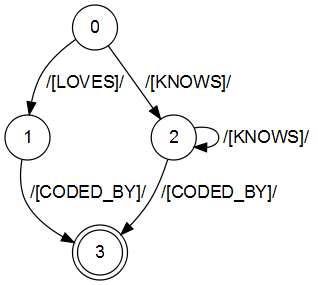
\includegraphics[width=0.5\textwidth]{img/automata-example}
\end{figure}
Now we try to match automata with the example graph (Figure ~\ref{fig:example-matrix}). The search is performed breadth-first by iterating through the graph and the query automata at the same time. A search state consists of the current node in the graph and the current position in the automaton. Different states could be at the same node in the graph, but in different states of the automaton, or vice versa. When we start traversing from one state, we check every edge starting from the current node in order to see if their labels are in the label set of the transitions starting from the current position in automata. When we reach the final state of the automaton, we add the starting node and current node in the graph to the answer set. We will store visited states and check if new states have been visited before every time. So the time complexity of BFS algorithm is $O(|V|*|S|)$ where $|V|$ and $|S|$ are number of nodes in graph and automata respectively as each state will be visited at most once.\\
\begin{figure}[h!]
  \caption{Example graph of MATRIX}
  \label{fig:example-matrix}
  \centering
    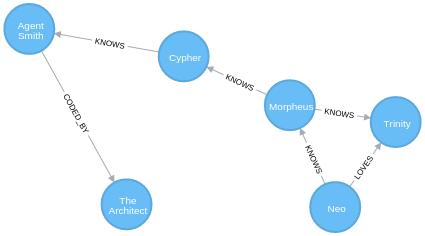
\includegraphics[width=0.8\textwidth]{img/matrix-graph}
\end{figure}
\begin{figure}[h!]
  \caption{Search Process for the automata in Figure \ref{fig:example-automata} }
  \label{fig:example-query-process}
  \centering
    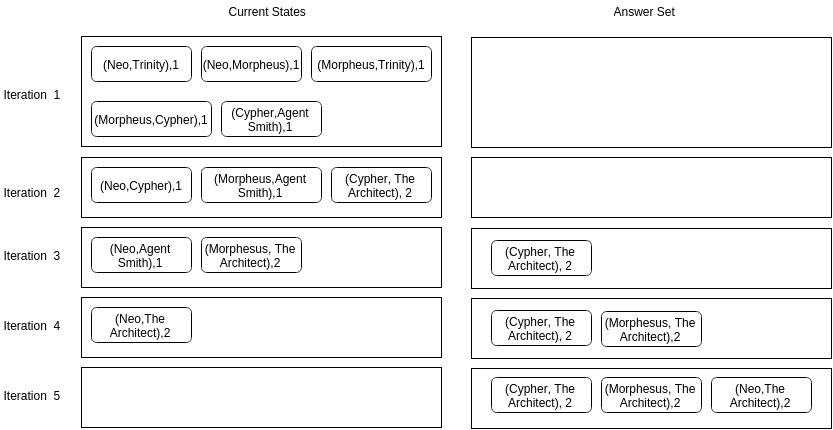
\includegraphics[width=1.0\textwidth]{img/Example-query-process}
\end{figure}
The search process is illustrated in Figure \ref{fig:example-query-process}:\\
For each state, the first pair such as $(Neo,Trinity)$ represents the start and end node in the graph, the second parameter like 1 or 2 represents the node position in automata. As the total number of visited states might be too large to show on this diagram, it's omitted here.
\subsection{Optimizations}
\subsubsection{Rare Labels}
Koschmieder and Leser propose a two-way BFS algorithm using rare labels in graph\cite{koschmieder2012regular}. The basic idea is to split the regular path query by rare labels and use them as fixed points to conduct two-way breadth first search. The rare labels would be determined by a user giving label frequencies.\\
The algorithm's advantages can be summarized as follows:
\begin{enumerate}
\item Rare labels occur much less in the graph, so we can reduce the search space when starting with rare labels.
\item For queries without matching pairs, we can achieve early stop by using rare labels.
\end{enumerate}
The algorithm can be done in 6 steps:
\begin{enumerate}
\item Locate all rare labels in the queries.
\item If there are more than one rare labels, find the paths between the first and second rare label, the second and third, etc.\ using a two-way search algorithm. If no path can be found in any of those search processes already, return an empty result set directly.
\item With the result from the previous step, find paths between the first and the last rare label.
\item From the first rare label, find all paths to the beginning of the regular expression.
\item From the last rare label, find all paths to the end of the regular expression.
\item Using the result from step 3, 4 and 5, generate all paths satisfying the regular expression and return the result set.
\end{enumerate}
For graphs with rare labels, the algorithm can speedup query evaluation by 90\%. However, if the graph or query contains no rare labels, the algorithm will still deteriorate to brute force search as introduced before. Furthermore, for many social network graphs, it's hard to define rare labels as there are only a limited number of labels and all of them are quite common.
\subsubsection{Path Index}
Peters' thesis work \cite{peters2015thesis} builds path indexes based on edge labels. A path index means for a specific path, or regular path expression, that we store all node pairs which meet the path. However, it's costly to store results for all possible paths for a graph, so Peter introduces the concept of k-path index, which means only paths of at most k steps will be stored.\\
For example, the 2-path index for example graph in Figure \ref{fig:example-matrix} would be:
\begin{table}[h!]
\def\arraystretch{1.5}
\centering
\caption{2-Path Index for MATRIX Graph}
\label{2-path-index}
\begin{tabular}{|l|m{20em}|}
\hline
Path            & Node pair                                                                \\
\hline
KNOWS           & (Neo,Morpheus), (Morpheus,Trinity), (Morpheus,Cypher), (Cypher,Agent Smith) \\
\hline
LOVES           & (Neo,Trinity)                                                            \\
\hline
CODED\_BY       & (Agent Smith, The Architect)                                             \\
\hline
KNOWS,KNOWS     & (Neo,Trinity),(Neo,Cypher),(Morpheus,Agent Smith)                             \\
\hline
KNOWS,CODED\_BY & (Cypher, The Architect)\\     
\hline
\end{tabular}
\end{table}
\\Peters adopts a similar approach with the rare label based algorithm and split the regular path query into smaller pieces according to histogram count of labels. Then for the sub-queries of relatively small size, path index could be looked up instead of searching graph, which saves time and I/O cost. Peters uses Postgres as back-end and elaborates carefully about the implementation details.\\
The limitation of path indexes shows when the query is long and the graph is dense, because then it might be very expensive to store the data structure. Moreover, in Peters' definition, the Kleene Star is not fully supported, instead lower and upper bound of the label occurrences is defined. 
\section{Distributed Evaluation of RPQ}
\subsubsection{Basic Definitions}
A distributed graph $DG$ is a graph whose nodes are partitioned into $m$ sets on $m$ sites. At each site $\alpha$, nodes and edges connecting them define a fragment $DG_\alpha$ of the distributed graph.\\
An edge $u\to v$ is called $cross-edge$ if $u$ and $v$ are stored on different sites.\\
For a cross-edge $u\to v$, $u$ is called output node, and $v$ is called input node.
\subsubsection{Algorithms}
The intuitive way to parallize RPQ evaluation is to query for each automata edge in parallel, then perform a multi-way join on the data. Again, to balance the search space and running time of algorithms, we can make use of fixed point strategy and search for sub-queries in parallel instead of searching for every automata edge at the same time. Dan Suciu has proposed an efficient algorithm\cite{suciu2002distributed} to evaluate RPQs on distributed graphs with distinguished properties as follows:
\begin{enumerate}
\item The number of communication steps is four, independent of the data and query.
\item The total amount of data exchanged during communication has the size of $O(n^2)+O(r)$, where 
$n$ denotes the number of cross-links in distributed database, $r$ the size of the result of the query.
\end{enumerate}
Dan's algorithm is improved by Tung, Nguyen-Van and Hu in \cite{tung2013efficient}, which decreases the data exchange size from $O(n^2)+O(r)$ to $O(|N|*|S|*|P|)$, where $N$ stands for number of input and output nodes, $S$ denotes number of nodes in automata, and $P$ is number of graph partitions.\\
Those two algorithms solve a more complex class of RPQ problems: they are trying to find all paths satisfying the given RPQ and only works on a rooted graph for semi-structure data such as XML. As the number of paths could be infinite in a cyclic graph and there might be multiple entry points for a graph, we will modify Dan's algorithm in section 4.
\section{Balanced Graph Partitioning}
As the data shuffled in distributed algorithms is related to graph properties such as number of input nodes or cross-edges, it's interesting to investigate how different partition strategies would affect the communication cost and try to optimize partition strategy for RPQ evaluation.\\
The balanced k-way graph partitioning can be defined as followed\cite{karypis1998multilevelk}: Given a graph $G = (V,E)$ with $|V| = n$, partition $V$ into $k$ subsets, $V_1,V_2,V_3,...,V_k$ such that $V_i\cap V_j=\emptyset$ for $i\neq j$, $|V_i|=n/k$ and the number of cross-edges is minimized. Here we require that the node size of each partition is the same as we want load balancing for query engine and using storage back-end that balance data over nodes such as Cassandra.\\
The direct computation of a good k-way partitioning is NP-hard problem\cite{karypis1998multilevel}, so the strategies in the survey below are all approximation algorithms.
\subsubsection{METIS}
METIS\cite{Karypis95metis} is a famous partitioning algorithm based on multilevel graph partitioning (MGP). MGP has three phases:
\begin{enumerate}
\item Shrink the graph to a smaller one by iteratively contracting edges and unifying nodes with four partitioning schemes in \cite{karypis1995multilevel}, which are:
    \begin{enumerate}
        \item Random Matching (RM): Each vertex coarsens with a random adjacent vertex.
        \item Heavy Edge Matching (HEM): Each vertex $u$ coarsens with an adjacent vertex $v$ such that the sum of edge weights $(u,v)$ is maximal.
        \item Light Edge Matching (LEM): Each vertex $u$ coarsens with an adjacent vertex $v$ such that the sum of edge weights $(u,v)$ is minimal.
        \item Heavy Clique Matching (HCM): Each vertex $u$ coarsens with an adjacent vertex $v$ such that the edge density is maximal. The motivation behind this scheme is to find highly connected components.
    \end{enumerate}
\item Partition the smallest graph after the graph is small enough to run a brute-force partitioning strategy inexpensively.
\item Bringing back the original graph by un-contracting edges and splitting the nodes. At the same time, do some local optimization to minimize edge cut.
\end{enumerate}
Although there are also other implementations based on MGP, such as KaFFPa\cite{sanders2011engineering} or \cite{soper2004combined}, in this project we select METIS as it has the fastest available parallel code and stable library. In this library, all of those four partitioning schemes mentioned above are applied and selected with smart policy according to the situation.
\subsubsection{JabeJa}
JabeJa\cite{rahimian2013jabeja} is a distributed balance partitioning algorithm which works in a different way from METIS: A k-way partitioning can be given with the help of a partition function $\pi$ which assigns a color from set \{1,2,3,...,k\} to each node. Let the number of neighboring nodes of node $p$ be $x_p$ and $x_p(c) = |N_p(c)|$ be the number of neighbors nodes of p with color $c$. The energy of the graph could be defined as followed:
$$E(G,\pi) = \sum_{p\in V} (x_p-x_p(\pi_p))$$
Then we can formulate the problem of optimal partitioning $\pi^*$ as followed:
$$\pi^* = \arg \min_{\pi} E(G,\pi)  $$ where $|V(c_1)|=|V(c_2)| $ for $\forall c_1,c_2 \in \{1,2,3,...,k\}$.\\
JabeJa is an iterative algorithm based on this model. For each iteration, every node will try to swap color with its neighbor and check if the swap makes the global energy smaller. The nodes only need to calculate the local result, which means they do not need global information to make a decision. There are several local search operators:
\begin{enumerate}
\item Local: every node selects its direct neighbors to swap color.
\item Random: every node select random nodes in the graph to swap color.
\item Hybrid: every node firstly applies the Local operator, then applies the Random operator after reaching the local optimum.
\end{enumerate}
Each time the nodes will swap color, the total number of nodes with each color will remain the same, which means the partition will keep balanced during the whole process. It's not possible to prove that JabeJa could get the optimal partition, but it could be easily customized to be based on other properties like input nodes number.
% \section{Graph Signature}
% Graph signature is a technique which encodes labels of each node into a bit-string. In gstore system\cite{zou2011gstore}, it's introduced for matching SPARQL queries with wildcards on large RDF graph. The basic definition will be as followed:\\
% Suppose the size of different labels in graph is $M$, then for every edge $e$, the edge signature $eSig(e)$ would be a bit-string where $(H(eLabel)\%M)$ -th bit set to '1', where $H(eLabel)$ is the hash-value of $eLabel$.\\
% Given a vertex $v$ from the graph, the vertex signature $vSig(v)$ is a bit-string constructed in following way:
% $$vSig(v)=eSig(e_1)|eSig(e_2)|......|eSig(e_n)$$
% where the $eSig(e_i)$ is the edge signature which starts from node v and "|" is the bitwise operation OR.\\ Given a graph $G$ and query $Q$, we can turn them into graph signature G* and query signature Q* by replacing each node and edge with the corresponding signature. For example, for MATRIX graph and a query $KNOWS\&LOVES$, the Q* and G* would be:\\
% \begin{figure}[h!]
%   \caption{Example of graph signature}
%   \label{fig:example-signature}
%   \centering
%     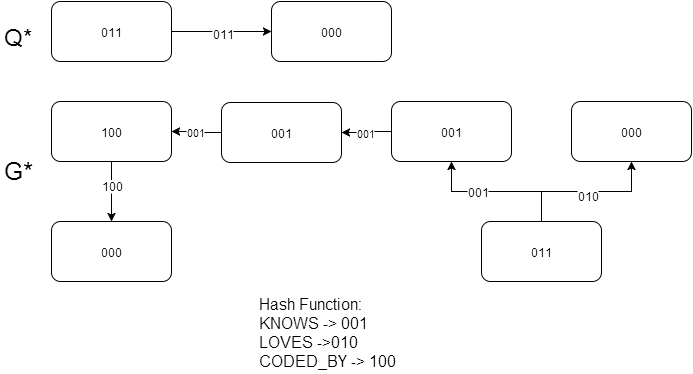
\includegraphics[width=0.8\textwidth]{img/signature-graph}
% \end{figure}
% \\Q* would be a sub-graph match for G* if and only if following conditions hold:\\
% \begin{enumerate}
% \item $vSig(v_i)\&vSig(u_i)=Vsig(v_i)$, i = 1,2,3,...,n, where '\&' is the bit-wise AND operator.
% \item If there is an edge from $v_i$ to $v_j$ in Q*, there is also an edge from $u_i$ to $u_j$ in G*.
% \end{enumerate}
% Although we cannot use this data signature in automata based RPQ evaluation directly, this technique could be useful while solving conjunctive regular path query. Comparing to Peter's index which is in depth-first way, the data signature is based on breadth-first principle. In section 5, we will illustrate how to build a vertex signature tree and combine it with distributed algorithm in order to accelerate CRPQ evaluation.e CRPQ evaluation. \chapter{\label{cha:exp-set}Experiment Setting}
\section{Data Model}
The Titan distributed graph database stores graphs under the BigTable data model as in figure \ref{fig:titan-data-model}.\\
\begin{figure}[h!]
  \caption{Titan Data Model\cite{data-model-titan}}
  \label{fig:titan-data-model}
  \centering
    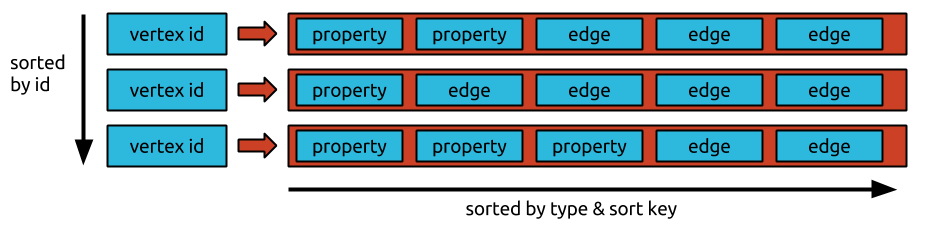
\includegraphics[width=0.8\textwidth]{img/titanstoragelayout}
\end{figure}
\\In this model, each row is identified by a unique vertex id, and the whole row stores the adjacency list of the vertex. Each edge or property is stored as an individual cell for efficient insertion and deletion. This data model fits back-ends such as Cassandra and HBase. In this thesis project for evaluating regular path queries, the column structure is defined according to edge labels. The basic data model is defined in figure \ref{fig:data-model}.\\
\begin{figure}[h!]
  \caption{Data Model}
  \label{fig:data-model}
  \centering
    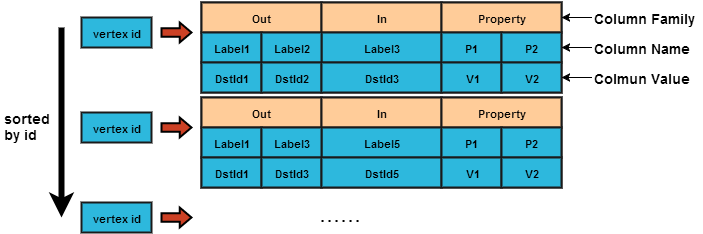
\includegraphics[width=0.9\textwidth]{img/data-model}
\end{figure}
\\In Titan, the edge label, edge direction(in/out) and destination id are encoded in column name together while Column Value only stores some other properties and meta-data. When evaluating the queries, Titan adopts features like prefix filter in HBase to locate edges and then decode information. In this project, the model can be simplified as not all the information is required for RPQ evaluation. Column Family is used to store edge directions and property. The Column Name stores an edge label or a single property name. The Column Value records destination vertices which are reachable with the label in Column Name. In the case of multiple destination vertices with the same label, the ids of vertices are encoded as a single value using a delimiter or put in 'Set' column value type of Cassandra. With this model, it's easier to group and locate columns by edge direction and edge labels.
\section{System Architecture}
All the programs are written in Scala 2.10 with necessary packages such as Spark-Cassandra-Connector. The versions of HBase and Cassandra are 0.98.6 and 2.1.5 respectively. The project is packaged with sbt, after which it is uploaded and run on cluster such as Google Cloud or SurfSara.
\subsection{Google Cloud}
In the early stage of this project, the system was deployed on top of Google Cloud Compute Engine. Spark runs in standalone mode as it can be tracked with WebUI directly. The cluster is fired up by the bdutil plugin with scripts starting Apache Spark and Apache HBase/Cassandra on each node. The configuration of the machines are in table \ref{machine-types}, as Spark is a memory-based computing framework, we reduce the impact of spilling by allocating as much memory as possible. The high-memory machine types are ideal for those tasks that require more memory relative to virtual CPUs. High-memory machine types have 6.50GB of RAM per virtual CPU.
\begin{table}[h!]
\def\arraystretch{2}
\centering
\caption{Machine Types}
\label{machine-types}
\begin{tabular}{l|l|l}
             & Master        & Worker        \\
\hline
Machine Type & n1-highmem-4 & n1-highmem-2 \\
\hline
Virtual CPUs & 4             & 2             \\
\hline
Memory(GB)   & 26            & 13          
\end{tabular}
\end{table}
\\For the n1 series of machine types, a virtual CPU is implemented as a single hardware hyper-thread on a 2.6GHz Intel Xeon E5 (Sandy Bridge), 2.5GHz Intel Xeon E5 v2 (Ivy Bridge), or 2.3 GHz Intel Xeon E5 v3 (Haswell).
\subsection{SURFsara Hadoop Cluster}
SURFsara is a Dutch foundation that provides supercomputers, colocation, networks and high-end visualisation to academic institutions. Its 'Hathi' Hadoop cluster consists of 170 data/compute nodes. These nodes have 1370 CPU-cores for parallel processing using YARN (MapReduce, Spark, Giraph). The system has a distributed file system with a capacity of 2.3 PB. Besides, it also has HBase cluster, which could be accessed by Spark Application on Yarn. Since the yarn cluster is in charge of allocating resources, I only give the params passed with spark-submit command:
\begin{table}[h!]
\centering
\caption{Parameters for Spark on Yarn}
\label{my-label}
\begin{tabular}{ll}
num-executors   & 1-64 \\
driver-memory   & 16GB \\
executor-cores  & 4    \\
executor-memory & 16GB
\end{tabular}
\end{table}
\subsection{System Structure}
After the setup, the system infrastructure is as shown in Figure \ref{fig:system-infra}. The Driver Program running on client machine connects to Cassandra seed node or HBase Master node in order to obtain information about database configuration. With the help of Cassandra-Spark-Connector\cite{spark-cassandra-connector} or HBaseRDD\cite{spark-hbase-connector} libraries, in each Spark Worker, a connection is opened which communicates with corresponding Cassandra node/HBase Region Server according to Config object in driver node. Usually, one Spark Worker is responsible for multiple regions as it has multiple cores and it's optimized to dispatch several spark partitions for one core. This architecture stores input/output files on Google File System or HDFS as the lower layer, which is omitted in the Figure \ref{fig:system-infra}.\\
\begin{figure}[h!]
  \caption{System Architecture}
  \label{fig:system-infra}
  \centering
    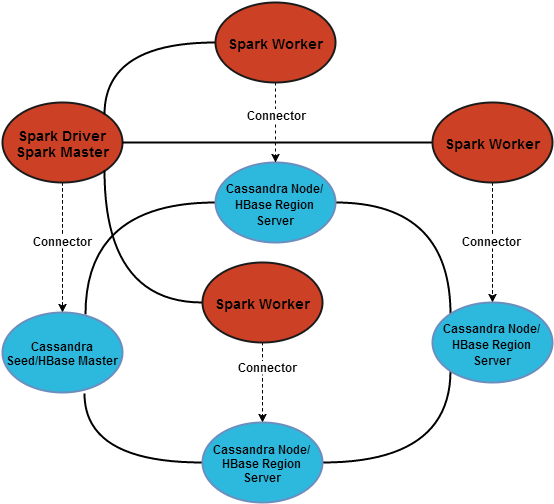
\includegraphics[width=0.8\textwidth]{img/system-architecture}
\end{figure}
\section{Benchmark}
In this project, we use both datasets from real-world and generated by the GMark Benchmark. Those graphs are all edge-labelled and have at least four kinds of edge-labels. All of them will be run against different partition strategies in Chapter 8, and Alibaba will be used for testing the RPQ evaluation algorithms in Chapter 7 as it has diverse labels. In following two sections, we present the properties of real-world datasets and parameters selected for the GMark Benchmark.
\subsection{Real-Datasets}
Alibaba is a graph which represents proteins and their interactions. It also comes with 12 regular path queries translated from biology and 10,000 random generated RPQ. YouTube extracts 15,088 users and their relations such as contact, shared friends, shared subscription, etc. The Higgs dataset has been built after monitoring the spreading processes on Twitter before, during and after the announcement of the discovery of a new particle with the features of the elusive Higgs boson on 4th July 2012. The messages posted in Twitter about this discovery between 1st and 7th July 2012 are considered. The basic statistics for those datasets are listed in Table \ref{real-datasets}.
\begin{table}[h!]
\def\arraystretch{2}
\centering
\caption{Real Datasets}
\label{real-datasets}
\begin{tabular}{|l|l|l|l|}
\hline
        & Nodes   & Edges      & Labels \\
\hline
Alibaba & 52,050  & 340,775    & 641    \\
\hline
YouTube & 15,088  & 13,629,182 & 5      \\
\hline
Higgs   & 456,626 & 14,855,842 & 4     \\
\hline
\end{tabular}
\end{table}
\subsection{GMark Benchmark}
The GMark Benchmark\cite{bagan2015controlling} generates both directed edge-labeled graph instances and query workloads coupled to those instances. It can control diversity of properties when generating graph and queries with user-defined schema. The authors are planning to align the benchmark with international benchmarking bodies such as the LDBC Council\cite{ldbc}.
\subsubsection{Graph Configuration}
The graph schema can be defined as a tuple $S = (\Sigma,\theta,\tau,\eta )$ where $\Sigma$ is a finite alphabet of predicates (i.e., edge labels), $\theta$ is a finite set of types such that each node of the generated graph is associated with exactly one type, $\tau $ is a set of constraints on $\Sigma$ and $\theta$ associating to each predicate and type either a proportion of its occurrence or a fixed constant value, and $\eta$ is a partial function associating to a triple consisting of a pair of input and output types $T_1,T_2$ in $\theta$ and a symbol $a$ in $\Sigma$, a pair $(D_{in})(D_{out})$ of in- and out-degree distribution.\\
A graph configuration $G=(n,S)$, where n is the number of nodes of the graph and S is the schema of the graph. In this experiments, we vary the number of nodes and keep the default graph schema in default configuration. The parameters are as followed:
\begin{enumerate}
    \item $n$: We vary the number of nodes from 100,000 to 10 million.
    \item $\Sigma$: In default settings, there are four predicates: authors, publishedIn, heldIn and extendedTo.
    \item $\theta$: There are 5 types of nodes. They are: researcher, paper, journal, conference and city.
    \item $\tau$: The constraints on predicates are: $\tau(authors)=0.5$, $\tau(publishedIn)=0.3$, $\tau(heldIn)=0.1$ and $\tau(extendedTo)=0.1$.\\ The constraints on types are: $\tau(researcher)=0.5$, $\tau(paper)=0.3$, $\tau(journal)=0.1$, $\tau(conference)=0.1 $ and $\tau(city)=100$.
    \item $\eta$: There are four kinds of degree distribution by benchmark definition, which can be denoted as $g$, $u$, $z$ and $ns$, meaning $Gaussian$, $Uniform$, $Zipfian$ and $Non-specified$ distributions respectively.\\ The default settings are $\eta(researcher,authors,papers)=(g(3,1),z(100,2.5))$,\\ $\eta(paper,publishedIn, conference)=(g(40,10),u(1,1))$,\\ $\eta(paper, extendedTo, journal)=(z(100,2.5),u(0,1))$ and \\$\eta(conference, heldIn, city)=(z(100,2.5),u(1,1))$
\end{enumerate}
\subsubsection{Query Configuration}
A query workload configuration can be represented as a tuple $Q = (G, \#q, ar, f, e, p_r, t)$ where $G$ is a graph configuration, $\#q$ is the number of queries in the workload, $ar$ is the arity constraint, $f$ is the shape constraint, $e$ is the selectivity of the queries in the workload, $p_r$ is the probability of recursion, and $t$ is the query size.\\
Again, we build our own configuration based on default settings, and the basic principle is not to change the parameter without a specific reason:
\begin{enumerate}
    \item $\#q$: By experience, each query takes from several seconds to several minutes. So 100 would be a reasonable number for each graph.
    \item $ar$: Arity constraint, which is the number of variables in RPQ. I choose 2 here as by definition RPQ contains 2 variables.
    \item $p_r$: Probability of Kleene star, which I set to 0.5, meaning half recursive queries and half non-recursive queries.
    \item $f$: Shape of RPQ. Since there can be 1 conjunct at most, star mode is the only choice.
    \item $e$: The estimated number of result comparing to graph size returned by RPQ, which has four options: Empty, Constant, Linear and Quadratic. For this part by default only Empty and Linear are enabled. To cover all cases, I enabled all of them.
    \item $t$: The query size can be represented as a tuple $$t=([c_{min},c_{max}],[d_{min},d_{max}],[l_{min},l_{max}])$$
    \subitem $[c_{min},c_{max}]$: Lower and Upper bound for number of conjuncts. I choose [1,1] as we are dealing RPQ but not CRPQ or UCRPQ here.
    \subitem $[d_{min},d_{max}]$: Number of disjuncts in RPQ, I keep the default configuration [1,3].
    \subitem $[l_{min},l_{max}]$: Length range of each atom element inside each disjunct. I also keep the default configuration [2,4].
\end{enumerate} \chapter{\label{cha:two-way}Cascaded Two Way Join}
An edge $(a,r,b)$ could be modelled as an instance of binary relation $R(A,B)$, and $S(B,C)$ for edge $(b,s,c)$. Then the searching process for a path from $a$ to $c$ in two steps could be expressed as a two way join process $R(a,b) \bowtie S(b,c)$. In Map-Reduce or Spark environment, the popular implementation is to map tuple $(a,b)$ and $(b,c)$ to key-value pairs $(b,(a,b))$ and $(b,(b,c))$, then reduce by key b. Specifically, the Join operation in Spark basically encapsulates the map-reduce process of two-way join.
\section{Query Plan}
In searching algorithm for regular path query, every search variable $A$ or $B$ in above cases consists of two nodes: one in graph and the other in automata. The two-way join operation could be expressed as follows:
\begin{enumerate}
    \item If there exists an edge $(1,r,2)$ in automata and an edge from $(a,r,b)$ with same label in graph, we can take the super-edge $((1,a),r,(2,b))$ as an instance of a binary relation $R(A,B)$, where $A$ and $B$ are search states variables. Similarly, we can get a super-edge $((2,b),s,(3,c))$ for the binary relation $S(B,C)$.
    \item Map super-edges to $((2,b),(1,a))$ and $((2,b),(3,c))$ key-value pairs with $(2,b)$ as the keys and $(1,a)$ or $(3,c)$ as values.
    \item Reduce two pairs by keys and combine values to new search states $((1,a),(3,c))$. Here we define the search states as a pair of two pairs, each of which contains  starting or current nodes in automata and graph.
\end{enumerate}
By now, there is only data parallelism in this process. In order to increase the power of parallelism, we can safely aggregate some edges with different labels to the same relation, which leads to query parallelism to some extent. In order to achieve that, we conduct a breadth first search on the automaton, and assign edges of each iteration to corresponding steps in the query plan.\\
For example, the query plan for automata in Figure \ref{fig:example-automata} is in table \ref{query-plan-example}.
\begin{table}[h!]
\centering
\caption{Query Plan Example}
\label{query-plan-example}
\begin{tabular}{ll}
step & edges                                                                 \\
0    & \begin{tabular}[c]{@{}l@{}}(0,LOVES,1) (0,KNOWS,2)\end{tabular}     \\
1    & \begin{tabular}[c]{@{}l@{}}(2,KNOWS,2) (1,CODED\_BY,3) (2,CODED\_BY,3)\end{tabular}                                                         \\
2    & \begin{tabular}[c]{@{}l@{}}(2,KNOWS,2) (2,CODED\_BY,3)\end{tabular} \\
3    &  \begin{tabular}[c]{@{}l@{}}(2,KNOWS,2) (2,CODED\_BY,3)\end{tabular}\\
4    & ...                                                                  
\end{tabular}
\end{table}
\\Then the whole search process is modelled as cascaded two-way joins:
$$(((R_0(A_0,A_1)\bowtie R_1(A_1,A_2))\bowtie R_2(A_2,A_3))\bowtie R_3(A_2,A_3))\bowtie...$$
where each $R_i$ contains edges of step i in query plan and $A_i$ represents pairs of nodes $(node_{automata},node)$. Note that the search will not end at stopping states of the automaton as there might be more edges starting from them.\\
The work $W(|V|)$ of this algorithm is $O((|V||S|)^2)$ where V is number of nodes in graph and S is number of states in the automaton. The time step $T_p = O(N)$ where $N$ is the number of relations $R_i$.\\
Assume $r_i$ is the size of relation $R_i$ and the match probability with $R_{i+1}$ is $p_{i}$, the input of first step is $r_1+r_2$, the output is $r_1*r_2*p_1$. The input for second step is of size $r_1*r_2*p_1+r_3$, the output size is $r_1*r_2*r_3*p_1*p_2$ ..., so the final input size is $\prod_1^{N-2}{r_i}*r_{N-1}+r_{N}$ and output size is $\prod_1^{N-1}{r_i p_i} *r_N$. The total network communication then is bounded by the sum of all the input and output sizes.

\section{Execution Process}
The execution process of cascaded two-way joins implemented in Apache Spark is as in diagram \ref{fig:two-way-join-spark}:
\begin{figure}[h!]
  \caption{Execution Process of Two-Way Join}
  \label{fig:two-way-join-spark}
  \centering
    \includegraphics[width=1.0\textwidth]{img/Two-way-join}
\end{figure}
\\The diagram depicts the main data-sets and the transform/action operation in Spark. As it's assumed that the graph cannot be loaded into memory at once, edges are loaded from HBase and stored in Resilient Distributed Dataset (RDD) only when they are needed. The process can be described in following steps: 
\begin{enumerate}
    \item Load automata edges from starting states in HDFS and retrieve edges which have same labels in HBase. Then join two RDD by labels, merge values to an RDD of search states. Use the dstid (Destination ID) in graph and automata as key.
    \item Count the size of search states RDD. If this equals 0, stop searching. Otherwise, filter those search states which begin with starting state and end in stopping states in automata. Merge the CurrentStates to VisitedStates by Union operation in Spark.
    \item Load Edges in automata for next step in the query plan, then retrieve graph edges by labels. Join two RDD by keys and merge values into a new RDD of search states with starting states as key.
    \item Join the two RDDs containing states of the current step and the next step, put the results into CurrentStates, using dstid as key.
    \item Subtract VisitedStates from CurrentStates, then go back to step 2.
\end{enumerate}
Since the number of transitions in the automaton is relatively small (less than 100), the main possible bottleneck is step 4, where two RDD of searching states are joined. As we use search state as key, the maximum number of reducing task is $(|V||S|)^2$ in step 4 every time. The RDD marked with red color is the one that got cached as it's referenced for several times and we don't want to recalculate it consistently.
 \chapter{\label{cha:multi-way}Multi-Way Join}
Similar to the Cascaded 2-way Join, the Multi-way Join searches by joining search states, except the it joins several relations at once.\\
Recall the number of reducing task is $(|V||S|)^2$ in every 2-way join step, if every state is a distinct key, the number of reducing tasks can be really huge: $O((|V||S|)^{2N})$ where $N$ is the number of relations $R_i$.\\ 
Afrati and Ullman\cite{afrati2010optimizing} solved this problem by giving each variable $A_i$ in relation a bucket number and setting their product equal to a given number $k$, which is usually the number of processors. Assume there are $N$ variables, then the key for each reducing process would consist of $N$ sub-keys. Each sub-keys $sb_i$ ranges from 1 to the bucket size $a_i$ for shared variable $A_i$.\\
For a relation instance $R_i(t_{i-1},t_i)$, the corresponding bucket is $(h(t_{i-1}),h(t_i))$ where $h$ is a hash function. As a consequence, the tuple $(t_{i-1},t_{i})$ is dispatched to all processes with sub-key $(h(t_{i-1}),h(t_i))$. As each edge would be broadcasted to several reducing processes, there is data redundancy during the process. The number of tuples passed to Reduce processes is:
$$\sum\tau_i$$
where $\tau_i$ is the product of $r_i$ (the number of tuples in $R_i$) times the product of those bucket sizes $a_j$ such that $A_j$ does not appear in the schema of $R_i$.
 After distributing all edges, each reduce task conducts cascaded joins locally. As it's crucial to decide number of buckets for each variable $A_i$ based on the size of each relation $R_i$, a Lagrangean equation is used to tackle the problem. Many formulas are given for different join types in Afrati's work, and regular path query evaluation can be modelled as chained mode:
$$R_0(A_0,A_1)\bowtie R_1(A_1,A_2)\bowtie R_2(A_2,A_3)\bowtie R_3(A_2,A_3)\bowtie...$$
The original Lagrangean equation for chain joins are as followed:
$$A_1 => \tau_3 + \tau_4 + ... + \tau_n = \lambda k$$
$$A_2 => \tau_1 + \tau_4 + ... + \tau_n = \lambda k$$
$$A_3 => \tau_1 + \tau_2 + \tau_5 + ... + \tau_n = \lambda k$$
$$A_4 => \tau_1 + \tau_2 + \tau_3 + \tau_6... + \tau_n = \lambda k$$
$$...$$
 Each variable $A_i$ has a differential equation, and by subtracting each equation with the former one, the following equations will be constructed:
$$\tau_1 = \tau_3 = \tau_5 = ...$$
$$\tau_2 = \tau_4 = \tau_6 = ...$$
and by applying the definitions of $\tau_i$, we get the following result for even $n$:
$$\frac{r_1}{a_1} = \frac{r_3}{a_2a_3} = \frac{r_5}{a_4a_5} = ... = \frac{r_{n-1}}{a_{n-2}a_{n-1}}$$
$$\frac{r_2}{a_1a_2} = \frac{r_4}{a_3a_4} = \frac{r_6}{a_5a_6} = ... = \frac{r_{n}}{a_{n-1}}$$
The formula for odd n is similar and will be discussed later.\\
According to Afrati's work\cite{afrati2010optimizing}, the $a_2$ for even-n is:
$$a_2 = (\prod_{j=2}^{n/2}\frac{r_2r_{2j-1}}{r_1r_{2j}})^{2/n}$$
The $a_2$ only depends on length of chain, which means $a_2$ is a known value immediately. The formula to calculate $a_{2i}$ is:
$$a_{2i} = (a_2)^i\prod_{j=2}^i\frac{r_1r_{2j}}{r_2r_{2j-1}}$$
which implies all even subscripts variable are known values. The formula for $a_{2i+1}$ is:
$$a_{2i+1} = \frac{a_1r_{2i+1}}{r_1a_{2i}}$$
In the end, the product of the shared variables could be written in form of $a_1$:
$$k = a_1^{n/2}\prod_{j=1}^{\frac{n-2}{2}}\frac{r_{2j+1}}{r_1}$$
Formulas for variables in odd-n in terms of $a_2$ are:
$$a_{2i} = (a_2)^i\prod_{j=2}^i\frac{r_1r_{2j}}{r_2r_{2j-1}}$$
$$a_{n-2i} = (a_2)^i\prod_{j=1}^i\frac{r_1r_{n-2j+1}}{r_2r_{n-2j+2}}$$
The product in terms of $a_2$ will be:
$$k = (\frac{a_2r_1}{r_2})^{\frac{n^2-1}{4}}\prod_{i=1}^{\frac{n-1}{2}}\prod_{j=1}^{i}\frac{r_{2j}r_{n-2j+1}}{r_{2j-1}r_{n-2j+2}}$$
\section{Removing Recurrence}
When dealing with recursive queries, the number of relations or query plan steps is unknown. For cascaded 2-way join, it's not necessary to calculate the number of edges in next step until finishing current iteration, so this is not a problem as application always know when to stop. However, we need number of $R_i$ and their size $r_i$ to solve Lagrangean equations in multi-way join, which requires a known query plan before start searching process.\\
The solution is to find the a spanning arborescence, which is a rooted and directed tree, where there's exactly one path from root to every other node. We find the arborescence of minimum weight of automata, which leads to a known query plan, and conduct cascaded 2-way joins between the search result of arborescence and the rest edges in automata.\\
For instance, the automata in \ref{fig:example-automata} can be compiled as followed:
\begin{table}[h!]
\centering
\caption{Query Plan Example For Multi-way Join}
\label{query-plan-multiway-example}
\begin{tabular}{ll}
step & edges                                                                 \\
0    & \begin{tabular}[c]{@{}l@{}}(0,LOVES,1) (0,KNOWS,2) (1,CODED\_BY,3)\end{tabular}     \\
1    & \begin{tabular}[c]{@{}l@{}}(2,KNOWS,2) (2,CODED\_BY,3)\end{tabular}                                                         \\
2    & \begin{tabular}[c]{@{}l@{}}(2,KNOWS,2) (2,CODED\_BY,3)\end{tabular} \\
3    &  \begin{tabular}[c]{@{}l@{}}(2,KNOWS,2) (2,CODED\_BY,3)\end{tabular}\\
4    & ...                                                                  
\end{tabular}
\end{table}
\\In step 0, the edges are from minimum spanning arborescence, and are joined in one go.
As a side effect of cascaded 2-way join in each reduce task, the visited states of each task are yielded. The states which end at the starting state in the next step are filtered from visited states. In this example, all states which end at state 2 are filtered and used for the starting states in step 1, as all edges there start with state 2.
\section{With Shared Variable Less Than 1}
One issue while solving those equations is that in some solutions some variables are less than 1, which is meaningless as we need positive integers for the bucket size.\\
Assume one shared variable $a_i$ is less than 1, then we set it to be 1 and remove it from map-key. If two consecutive variables $a_{i-1}$ and $a_{i}$ are less than 1 at the same time, $R_i$ will be removed from the calculation as all edges of $R_i$ should be broadcasted to all processes. Assume after removing consecutive variables and corresponding relation, each relation should at most have one variable less than 1. It's natural to cut the original chain into two sub-chains by variable less than 1. The Lagrangean equations are modified as followed after removing the equation of $a_i$:
$$a_1 => \tau_3 + \tau_4 + ... + \tau_n = \lambda k$$
$$a_2 => \tau_1 + \tau_4 + ... + \tau_n = \lambda k$$
$$a_3 => \tau_1 + \tau_2 + \tau_5 + ... + \tau_n = \lambda k$$
$$...$$
$$a_{i-1} => \tau_1 + \tau_2 + ... \tau_{i-2} + \tau_{i+1} + ... + \tau_n = \lambda k$$
$$a_{i+1} => \tau_1 + \tau_2 + ... \tau_{i} + \tau_{i+3} + ... + \tau_n = \lambda k$$
$$...$$
As a result the two equations $\tau_{i-1} = \tau_{i+1}$ and $\tau_{i} = \tau_{i+2}$ will not hold anymore, instead if we subtract equations of $a_{i-1}$ and $a_{i+1}$, a new equation will be formed:
$$\tau_{i-1} + \tau_{i} = \tau_{i+1} + \tau_{i+2}$$
which could be rewritten as:
$$\tau_{1} + \tau_{2} = \tau_{i+1} + \tau_{i+2}$$
In general we have one less equation as well as one less variable, so the equations for shared variables are still solvable.\\
The equations for shared variable would be like followed with even i:
$$\frac{r_1}{a_1} = \frac{r_3}{a_2a_3} = ... =  \frac{r_{i-1}}{a_{i-2}a_{i-1}} \neq \frac{r_{i+1}}{a_{i+1}} = ... = \frac{r_{n-1}}{a_{n-2}a_{n-1}}$$
$$\frac{r_2}{a_1a_2} = \frac{r_4}{a_3a_4} = ... = \frac{r_i}{a_{i-1}} \neq \frac{r_{i+2}}{a_{i+1}a_{i+2}} = ... = \frac{r_{n}}{a_{n-1}}$$
When solving equation $\tau_{1} + \tau_{2} = \tau_{i+1} + \tau_{i+2}$, there are three cases for the length of each sub-chain: EVEN-EVEN, ODD-ODD and EVEN-ODD(ODD-EVEN).
For a sub-chain of even length, the $\tau_{1} + \tau_{2}$ can be expressed as $\frac{r_1+r_2/a_2}{a_1}$. Since $a_2$ is a known value, the result only depends on value of $a_1$.\\
For a sub-chain of odd length, the $\tau_{1} + \tau_{2}$ is $ C* ( r_1/a_2^{(n-1)/2}+r_2/a_2^{(n+1)/2} )$ where $C = \prod_{j=1}^{\frac{n-1}{2}}\frac{r_1r_{n-2j+1}}{r_2r_{n-2j+2}}$ and n is the length of sub-chain.\\
With the formulas above, it's possible to solve the equation $\tau_{1} + \tau_{2} = \tau_{i+1} + \tau_{i+2}$ between representative shared variable in sub-chains, which could be either $a_1$ or $a_2$ according to the length of sub-chain:
$$EVEN-EVEN : \frac{r_1+r_2/a_2}{a_1} = \frac{r_{i+1}+r_{i+2}/a_{i+2}}{a_{i+1}}$$
$$ODD-ODD :C_1* ( r_1/a_2^{(i-1)/2}+r_2/a_2^{(i+1)/2} ) = C_2* ( r_{i+1}/a_{i+2}^{(n-i-1)/2}+r_{i+2}/a_{i+2}^{(n-i+1)/2} ) $$
$$EVEN-ODD : \frac{r_1+r_2/a_2}{a_1} = C_2* ( r_{i+1}/a_{i+2}^{(n-i-1)/2}+r_{i+2}/a_{i+2}^{(n-i+1)/2} )$$
The ODD-EVEN situation is similar to EVEN-ODD, in which case we just need to swap the content on different sides.\\
For example, in the case of EVEN-EVEN, it's possible to represent sub-product of each sub-chain in the form of only one variable $a_1$ and equal the product of sub-products to k:
$$k = a_1^{i/2}\prod_{j=1}^{\frac{i-2}{2}}\frac{r_{2j+1}}{r_1}*(\frac{r_{i+1}+r_{i+2}/a_{i+2}}{r_1+r_2/a_2}a_1)^{(n-i)/2}\prod_{j=1}^{\frac{n-i-2}{2}}\frac{r_{i+2j+1}}{r_{i+1}}$$
After solving the value of $a_1$, $a_{i+1}$ can be calculated, thus all variables in sub-chains can be obtained.\\
For example, the query $ [1]^*[0][471][0][1]^+$ for Alibaba Benchmark, can be compiled into a query plan of 4 relations. The tuple of sizes is $(332642,2,306617,26025)$, for the first iteration, the shared variables are $(1.0,11.784072,0.008416,1290.581264,1.0)$ respectively assuming $k=128$. The first and last variable are set to $1.0$ as they are dominated. However, the $a_2$ is much less than 1 and $a_3$ is much larger than $k$. This is caused by the massive difference between the relation size of $r_2=2$ and other relations. According to the method above, we remove $a_2$ and recalculate the shared variables. The new tuple is $(1.0,11.313741,1.0,11.313741,1.0)$, which can be rounded to $(1.0,12.0,1.0,12.0,1.0)$. The product of all shared variables is slightly larger than $k$, which is tolerable here. Then, for shared variables $a_1$ and $a_3$, the bucket sizes are both 12, and every other variable only has one bucket.
\subsubsection{General Cases}
In case there are multiple variables $a_{i_1},a_{i_2}...a_{i_m}$ which are less than 1, the chain join will be cut into several sub-chains. The similar process will be applied to every sub-chain and its following sub-chain. Then the product of sub-products can be expressed in form of $a_1$ and equals to k. With solved $a_1$ or $a_2$, the values $a_{i_1+1},a_{i_2+2}...,a_{i_m+1}$ can be calculated from EVEN-EVEN, ODD-ODD or EVEN-ODD formula one by one.
\subsubsection{Implementation}
Basically there are two ways to implement with shared variables less than 1:
\begin{enumerate}
\item Split $k$ and dispatch results to sub-chains. For example, if $k$ = 64, we assign $k_1 = 8$ and $k_2 = 8$ to each sub-chain. This is easier for coding but not really accurate. In fact the connection between different sub-chains are cut off and we are solving completely different sub-problems.
\item Binary search the value of $a_1$ or $a_2$ between 1 and $k$. For the variables on different sides in EVEN-EVEN, ODD-ODD or EVEN-ODD formulas, they are monotonic with each other, which makes binary search applicable. Every time we assign a value to $a_1$ or $a_2$ and then get temporary $a_{i+1}$ or $a_{i+2}$, leading to sub-product $k_1$ and $k_2$. Then we adjust the value of $a_1$ or $a_2$ after checking the relation between $k_1*k_2$ and k.
\end{enumerate}
\section{Execution Process}
The execution process of cascaded multi-way joins implemented in Apache Spark is as in diagram \ref{fig:multi-way-join-spark}:
\begin{figure}[h!]
  \caption{Execution Process of Multi-Way Join}
  \label{fig:multi-way-join-spark}
  \centering
    \includegraphics[width=0.8\textwidth]{img/Multi-way-join-process}
\end{figure}
\begin{enumerate}
    \item Load all edges in automata to RDD, named as AllTransitions. Retrieve edges from HBase to RDD by edge labels in AllTransitions, naming the RDD AllEdges with the edge label as key.
    \item Build arborescence based on AllTransitions and join with AllEdges, which yields the states before break points in automata. We call the new RDD AllStates. As the same edge can be used in multiple relations, we set the step number in query plan as the key.
    \item With the help of a histogram of labels, we can compile the query plan and calculate bucket sizes for each query step according to formulas. The bucket numbers form the key space and are flat-mapped with AllStates.
    \item Dispatch states to reduce tasks according to $(h((dstid,dstid)),h((srcid,srcid)))$.
    \item Each reduce task conducts local cascaded search and stores all visited states into VisitedStates.
    \item Now the Multi-way Join part is almost done, after which a parallel cascaded 2-way join will be applied to states starting from break points in the automaton. All Edges and AllTransitions are still used in cascaded 2-way join as it's possible to search back to edges in the Arborescence RDD. VisitedStates is also referred in cascaded 2-way join for removing duplicate states.
    \item Finally, with all produced VisitedStates, we filter all search states that begin with start states and end at stop states in the automaton.
\end{enumerate}
 \chapter{\label{cha:dan-alg}Dan Suciu's Algorithm}
When testing previous two algorithms against 1000 random simple queries without recursion from Alibaba dataset, it's observed that shuffle size can already be as large as several GBs. The reason behind it is that "join" transformation is a reduce-side join operation, so full shuffles happen a lot while joining states or edges. Recall the system architecture in Chapter \ref{cha:exp-set}, it would be great if we can make use of data locality during evaluation and reduce shuffling by doing local computation as much as possible.\\
Furthermore, the query parallelization in previous two algorithms is only considered when compiling a query plan where multiple edges are put into a single query step. However, the search still begins with the starting state of the automaton. It could be faster to start searching for multiple starting points when we have adequate computing resources.
\section{Epsilon Edges}
One trick to store and traverse graph in a distributed context is drawing cross-edges back into local partitions and adding epsilon edges between different sites. The example in Figure \ref{fig:empty-edges} explains the basic idea: for cross-edges $(u_1,v_1), (u_1,v_2), (u_2,v_2), (u_3,v_1)$ and $(u_3,v_3)$, we create virtual nodes $v_1', v_2'$ and $v_3'$ in red site, and adding epsilon edges between them and corresponding nodes in other sites.
\begin{figure}[h!]
  \caption{Adding Epsilon Edges between Sites}
  \label{fig:empty-edges}
  \centering
    \includegraphics[width=0.8\textwidth]{img/empty-edges}
\end{figure}
\\This partitioning technique can also be interpreted as vertex-cuts, which is adopted by popular graph processing frameworks such as GraphLab\cite{low2012distributed} and GraphX\cite{xin2013graphx}. By constraining every edge in a certain site, it's possible to achieve data and computation locality, which Dan Suciu's algorithm is based on.
\section{Original Dan Suciu's Algorithm}
In \cite{suciu2002distributed}, an algorithm is proposed by Dan Suciu to solve regular path queries on distributed rooted semi-structured data, and return all paths satisfying the RPQ. The algorithm is described in Algorithm 1:
\begin{algorithm}
    \SetKwInOut{Input}{Input}
    \SetKwInOut{Output}{Output}
    \Input{A semistructured database db distributed on a number of sites: db = $\cup_{\alpha}db_{\alpha}$, a regular path query R whose automaton is A}
    \Output{All paths t which satisfy R}
    initialization\;
    \textbf{Step 1} \\Send A to all servers $\alpha$, $\alpha = 1,...,m$\\
    \textbf{Step 2} \\At every site $\alpha$ let $F_a$ be $db_a$:\\
                        $Node(F_a)\leftarrow Node(db_a)$
                        $InputNode(F_a)\leftarrow InputNode(db_a)$
                        $Edges(F_a)\leftarrow Edges(db_a)$
                        $OutputNode(F_a)\leftarrow OutputNode(db_a)$
                        $visited_a\leftarrow\{\}$ \\
                    \ForAll {$r\in InputNodes(db_a),s\in States(A)$}{
                        $S\leftarrow visit_a(s,r) $\\
                        $InputNodes(F_a)\leftarrow InputNodes(F_a)\cup \{(s,r)\}$\\
                        \ForAll {$p\in S$}{
                            $Edges(F_a) \leftarrow Edges(F_a)\cup \{(s,r) \xrightarrow{\epsilon} p\}$
                        }
                    }
    \textbf{Step 3} \\At every Site $\alpha$ construct the accessibility graph for $F_a$.\\
    \textbf{Step 4} \\Every site $\alpha$ sends it accessibility graph to the master and compute the global accessibility graph at the master site.\\
    \textbf{Step 5} \\Broadcast the global accessibility graph to every server $\alpha$, $\alpha = 1,...,m$.\\
    \textbf{Step 6} \\Every site $\alpha$ computes $F_a^{acc}$, the accessible part of $F_a$.\\
    \textbf{Step 7} \\Every site $\alpha$ sends $F_a^{acc}$ to the master site, where it is assembled into result.
    \caption{Dan Scuciu's Algorithm}
\end{algorithm}
\begin{algorithm}
    \SetKwInOut{Input}{Input}
    \SetKwInOut{Output}{Output}
    \Input{A state $s$ in automata and a node $u$ in graph}
    \Output{A set of states which $(s,u)$ can reach in current site $\alpha$}
    \lIf{$(s,u)\in visited_a$}{
        \Return $result_a[s,u]$
    }
    $visited_a\leftarrow visited_a\cup \{(s,u)\}$\\
    $result_a[s,u]\leftarrow\{\}$\\
    \If{$u\in OutputNode_a(db_a)$}{
        $OutputNode_a(F_a)\leftarrow OutputNode_a(db_a)\cup \{(s,u)\}$\\
        $result_a[s,u]\leftarrow result_a[s,u]\cup \{(s,u)\} $
    }
    \lElseIf{ $s$ is a terminal state}{
        $result_a[s,u]\leftarrow \{u\} $
    }
    \ForAll{$u\xrightarrow{a}v$ in $Edges(db_a)$}{
        \lIf{$a=\epsilon$}{$result_a[s,u]\leftarrow result_a[s,u]\cup visited_a(s,v) $}
        \Else{
            \ForAll{$s\xrightarrow{P}s'$(*automata transition*)}{
                \If{$P(a)$}{$result_a[s,u]\leftarrow result_a[s,u]\cup visited_a(s',v) $}
            }
        }
    }
    \Return $result_a[s,u]$
    \caption{function $visited_a(s,u)$}
\end{algorithm}
\\Before running Algorithm 1, the graph is partitioned by the vertex cut approach. Theoretically there are only $\epsilon$ edges between different sites. In Algorithm 1,  step 1 broadcast edges of automata to all servers. Step 2 locates all $InputNodes$ and $OutputNodes$ in vertex-cut partitioned graph. Making use of Algorithm 2, every site starts visiting search states $(s,u)$ consisting of every input-node $u$ and every state in the automaton $s$, to states with ouput-node or final state in the automaton. For all states $(t,v)$ which can be reached from input search states $(s,u)$, we add $\epsilon$ edge between them. Similar to our approaches in previous sections, the accessibility graph constructed are formed by pairs $((s_i,u_i),(t_i,v_i))$. In step 4, we receive $\cup F_i,i=1,2,3...,m$ from all sites and conduct searching from root state $(s_1,r)$ to $(f,dstid)$ on it, where r is the root for $db$, $s_1$ is the starting state in the automaton and $f$ is the final state of the automaton. After computing the global accessibility graph, each state of which can be part of paths from $(s_1,r)$ to $(f,dstid)$, the global accessibility graph will be sent back to all servers in step 5. In step 6, each sites send back all paths in own site satisfying part of global accessibility graph and transmit them back to the master site in step 7. Finally, the master assembles all paths from $(s_1,r)$ to $(f,dstid)$.\\
As mentioned in research background, the main advantages of Dan Suciu's algorithm are:
\begin{enumerate}
    \item Known number of 4 communication steps, which are step 1, 4, 5, and 7.
    \item Total amount of data exchanged during communications has size $O(n^2)+O(r)$, where $n$ is the number of cross-edges (step 4) and r is the size of the query result (step 7).
\end{enumerate}
\section{Modified Dan Suciu's Algorithm}
The main differences between our RPQ definition and Dan Suciu's are as followed:
\begin{enumerate}
    \item The graphs we process are not necessarily rooted.
    \item We only need the pairs of starting and ending nodes, not all paths between them.
\end{enumerate}
For the first difference, we can add more starting states in step 2, and for the second one, we can remove step 5-7 from algorithm 1. Then the modified algorithm can be described as in Algorithm 3:
\begin{algorithm}
    \SetKwInOut{Input}{Input}
    \SetKwInOut{Output}{Output}
    \Input{A semistructured database db distributed on a number of sites: db = $\cup_{\alpha}db_{\alpha}$, a regular path query R whose automaton is A}
    \Output{All paths t which satisfy R}
    initialization\;
    \textbf{Step 1} \\Send A to all servers $\alpha$, $\alpha = 1,...,m$\\
    \textbf{Step 2} \\At every site $\alpha$ let $F_a$ be $db_a$:\\
                        $Node(F_a)\leftarrow Node(db_a)$
                        $InputNode(F_a)\leftarrow InputNode(db_a)$
                        $Edges(F_a)\leftarrow Edges(db_a)$
                        $OutputNode(F_a)\leftarrow OutputNode(db_a)$
                        $visited_a\leftarrow\{\}$\\
                        $StartNode\leftarrow\{\}$ \\
                    \ForAll {$u\in Nodes(db_a),s_1$}{
                            $S\leftarrow visit_a(s_1,u) $\\
                            $InputNodes(F_a)\leftarrow InputNodes(F_a)\cup \{(s_1,u)\}$\\
                            \ForAll {$p\in S$}{
                                $Edges(F_a) \leftarrow Edges(F_a)\cup \{(s_1,u) \xrightarrow{\epsilon} p\}$
                            }
                    }
                    \ForAll {$r\in InputNodes(db_a),s\in States(A)-\{s_1\}$}{
                        $S\leftarrow visit_a(s,r) $\\
                        $InputNodes(F_a)\leftarrow InputNodes(F_a)\cup \{(s,r)\}$\\
                        \ForAll {$p\in S$}{
                            $Edges(F_a) \leftarrow Edges(F_a)\cup \{(s,r) \xrightarrow{\epsilon} p\}$
                        }
                    }
    \textbf{Step 3} \\At every Site $\alpha$ construct the accessibility graph for $F_a$.\\
    \textbf{Step 4} \\Every site $\alpha$ sends it accessibility graph to the master and compute the global accessibility graph at the master site.
    \caption{Modified Dan Scuciu's Algorithm}
\end{algorithm}
\\The search function in Algorithm 2 is still the same. In Step2, we start searching with all nodes and starting state $s_1$ in automata. Since $s_1$ has been searched with all nodes in the current site, it's unnecessary to access them again for $InputNodes$.
\\As a result, there are only two communication steps: Step 1 and Step 4. Since the number of transitions in the automaton  is almost less than 100, broadcasting them to each site is relatively less expensive. So the main cost is from step 4, where each site sends its local accessibility graph to master. The total amount of data exchanged during communications is of size $O(n^2)+O(r)$ for Dan Suciu's algorithm, which is not very accurate for diverse benchmarks. For Algorithm 3, more data exchanged are introduced, which will be analyzed carefully in Evaluation step.
\section{Execution Process in Spark}
The execution process in Spark is presented as followed figure \ref{fig:dan-algorithm-spark}:
\begin{figure}[h!]
  \caption{Execution Process of Modified Dan Suciu's Algorithm}
  \label{fig:dan-algorithm-spark}
  \centering
    \includegraphics[width=0.8\textwidth]{img/dan-algorithm-spark}
\end{figure}
To avoid full shuffle, the automaton is treated as a broad-casted variable in Spark, and is involved in a map-side join on each partition of RDD. Similarly, the operation `subtract' or `union', which also perform full shuffle or need repartitioning at the low level, is replaced with operation "zipPartitions".
The process can be described in following steps: 
\begin{enumerate}
    \item Load automata transitions from HDFS and retrieve edges which have same labels in HBase. Then broadcast automata to each partition in the graph. Perform local join by the flatMap operation, which use the dstids (Destination ID) in graph and automata as key.
    \item Count the size of search states RDD, if equals 0, stop searching. Otherwise, filter the accessibility graph to send buffer. Zip each partition of search states to VisitedStates and merge each zipped partition.
    \item Load transitions for next step, then retrieve graph edges by labels. Broadcast transitions to partitions of edges. Then do local join by labels and merge values into a new RDD of search states with starting states as key.
    \item Zip two RDD of search states of current step and next step, conduct local join and merge the value into a new RDD of search states, using dstid as key.
    \item Zip new CurrentStates with VisitedStates by partition. For each zipped partition pairs, the partition from new states RDD filters the states which haven't appeared in the partition from VisitedStates, then go back to step 2.
    \item Send all search states in send buffer to driver node. The driver assembles local results into a global accessibility graph, then filters the search states starting from $s_1$ and ending with accept states.
\end{enumerate}

\chapter{\label{cha:evaluation}Evaluation}
\section{Approach}
In this section, we run Cascaded 2-way Join, Multi-way Join, and modified Dan Suciu's Algorithm against 35 queries selected from Alibaba Benchmark and compare the performance. The RPQs are translated into DFA by library \cite{hackingoff} from HackingOff.com, which implements Thompson's construction algorithm \cite{Thompson:1968:PTR:363347.363387}. We eliminate the complex queries which take more than 1 hour sequentially. The queries selected can take 10 seconds at least, and in average 1 minute sequentially. The program is deployed to cluster with 2, 4, 8, 16, 32 and 64 executors on Surf Sara. Unfortunately, sometimes the tasks were too heavy for 2 or 4 machines, leading to a zookeeper timeout/crash, which returns no result. So those parts were ignored when gathering data.
\section{Metrics}
The experiment data is collected from the Spark UI and event logs, and the metrics we focus on are:
\begin{enumerate}
    \item Running time: The time spent on evaluating a single query, including both executor and driver sides while taking parallelism into account. At the same time, we count average duration, maximum duration and minimum duration spent on a single query.
    \item Time Stack: By analyzing the event log of spark applications, the application runtime can be split into several parts:
        \begin{enumerate}
        \item Executor Computing Time: The average time each executor spends on the computation of action or transform steps.
        \item Shuffle Read/Write Time: The average time each executor spends on writing or reading shuffled data.
        \item Transforming Time: The average time each executor spends on de-serializing the tasks and serializing result.
        \item Scheduler Delay Time: The average time it takes to send task from scheduler to executor.
        \item JVM GC Time: The time spent on garbage collection.
        \end{enumerate}
    \item Shuffled data size: Most disk I/O and network communications happen during data shuffling. During shuffling data, Spark executors will write data to the local buffer in shuffle write phase, and based on the key of requested data, each executor reads data from the local buffer or remote buffer of other executors. 
    % \item Memory usage: We measure the peak memory usage of all executors. As Spark is a memory-based computing framework, it's crucial to monitor memory usage and avoid spilling data to disk, which would impact the performance.
\end{enumerate}
\section{Running Time}
Figure \ref{fig:Average-RunTime-for-Each-Alibaba-Query} depicts running time stats for those queries:
\begin{figure}[h!]
  \caption{Average Running Time Comparison}
  \label{fig:Average-RunTime-for-Each-Alibaba-Query}
  \centering
    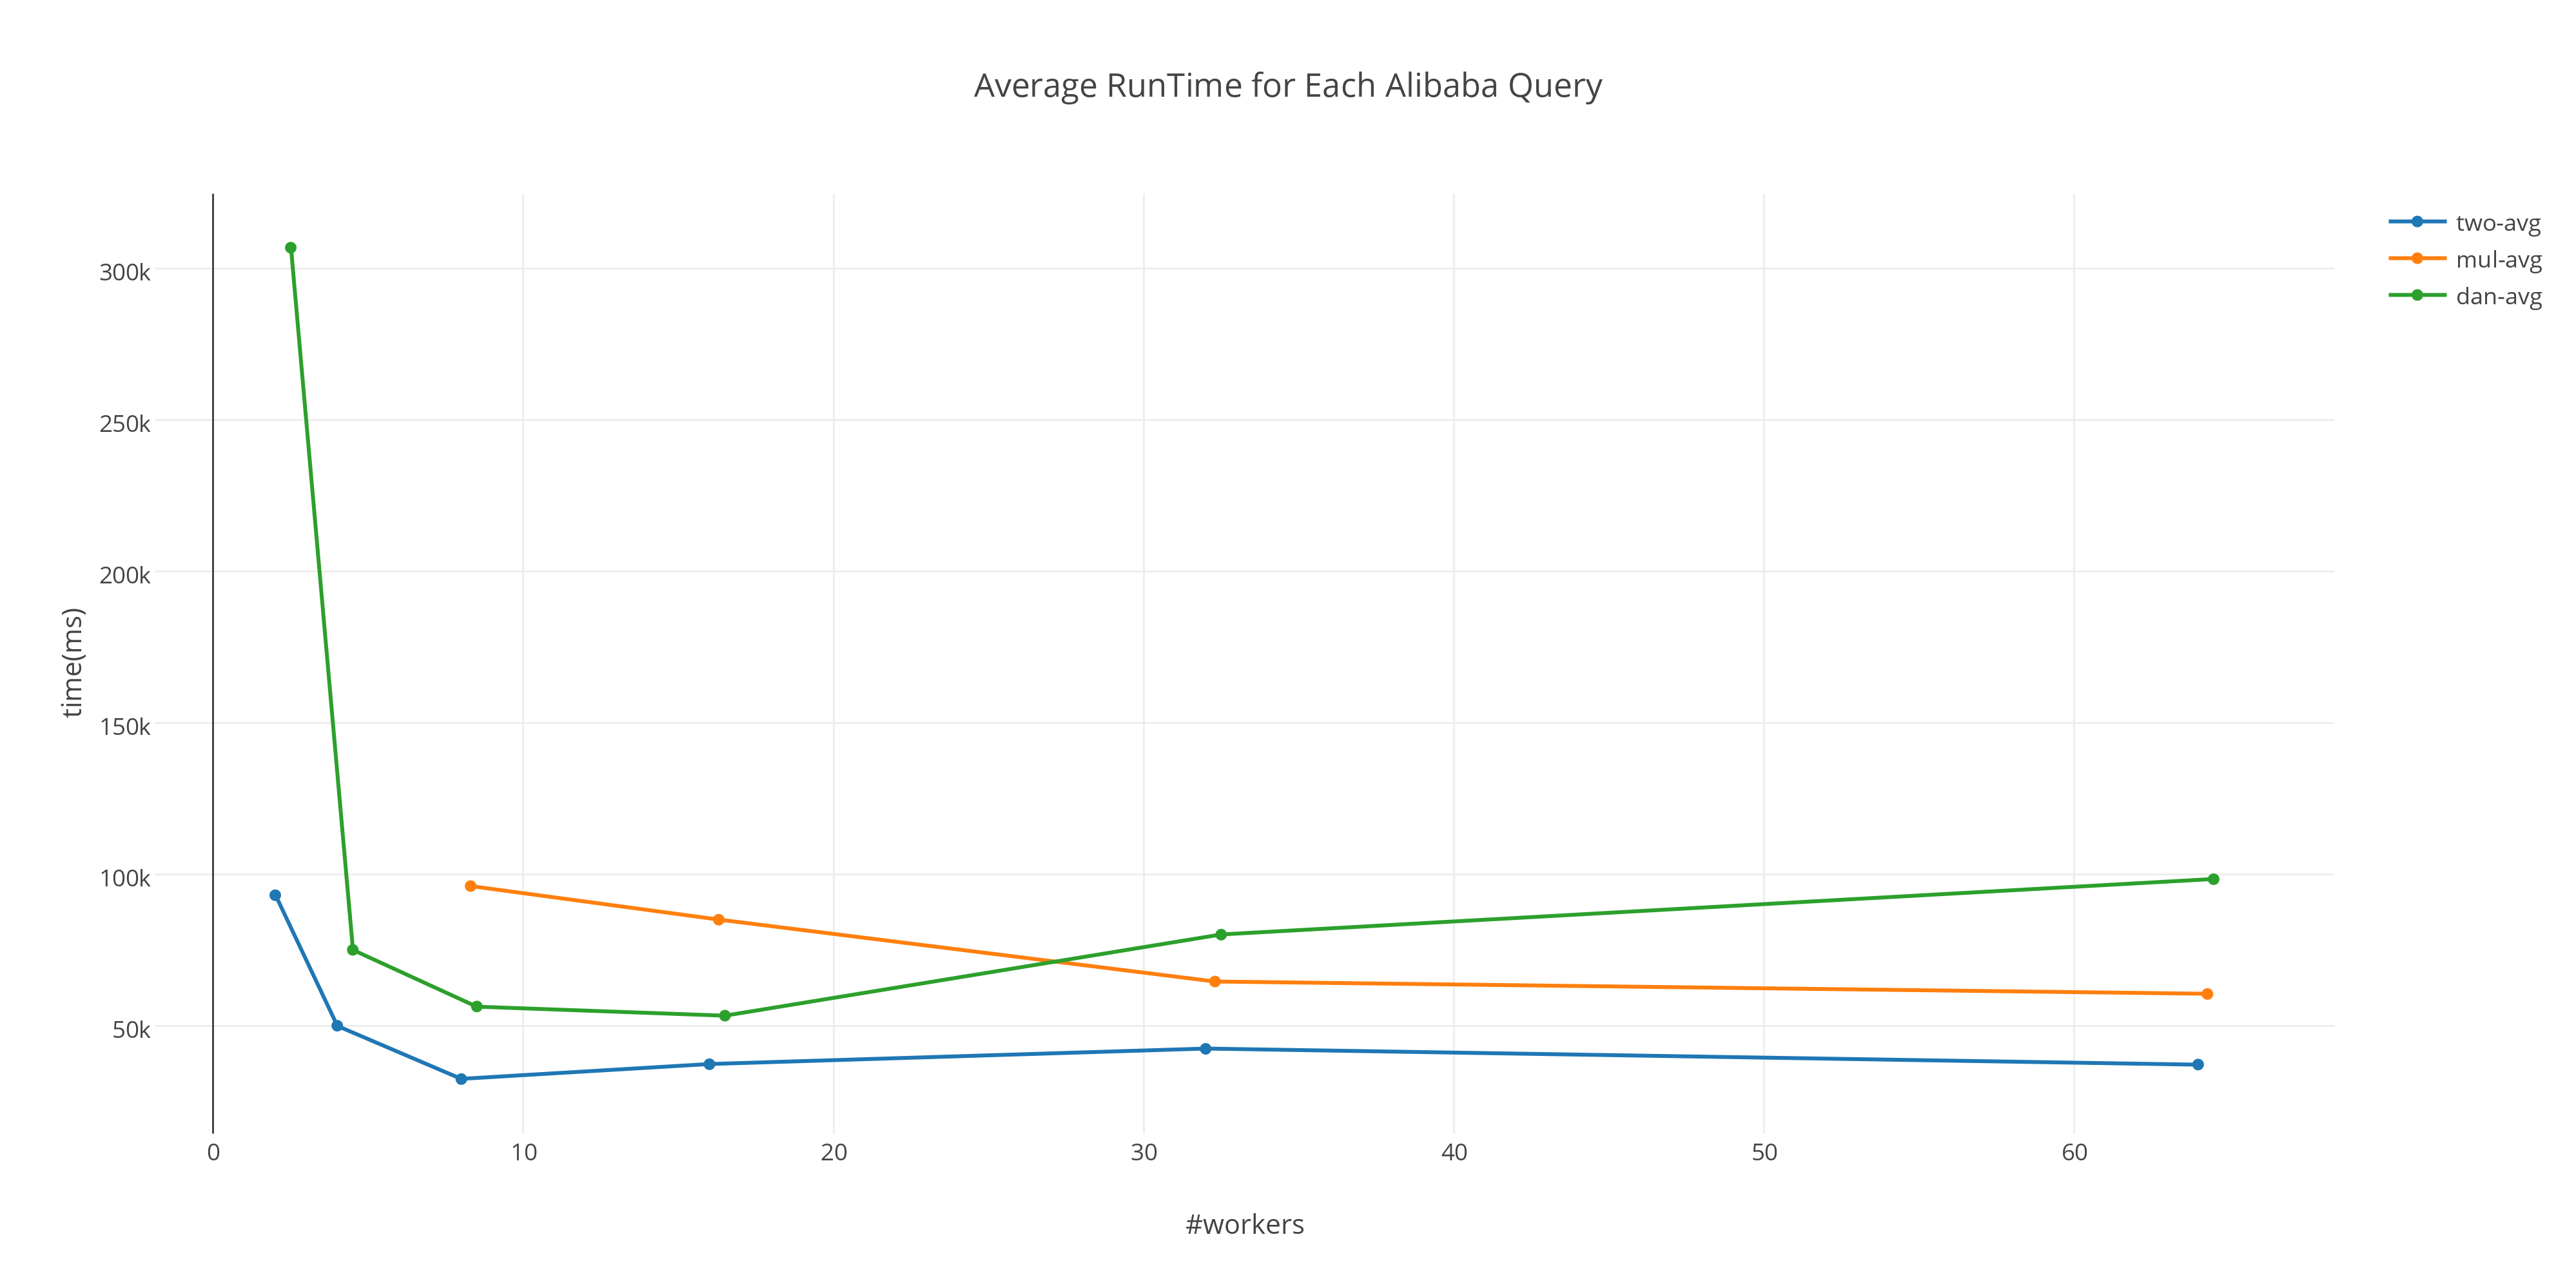
\includegraphics[width=1.0\textwidth]{img/Average-RunTime-for-Each-Alibaba-Query}
\end{figure}
\\The figure suggests cascaded two-way join is the most scalable and fastest solution for this benchmark. Dan Suciu's algorithm also has good speed up when the number of executors is less than 10. When the executor number is larger, the overhead introduced cannot be made up by speed-up already.
\begin{figure}[h!]
  \caption{Average Running Time of Two-Way Join}
  \label{fig:two-way-join-general}
  \centering
    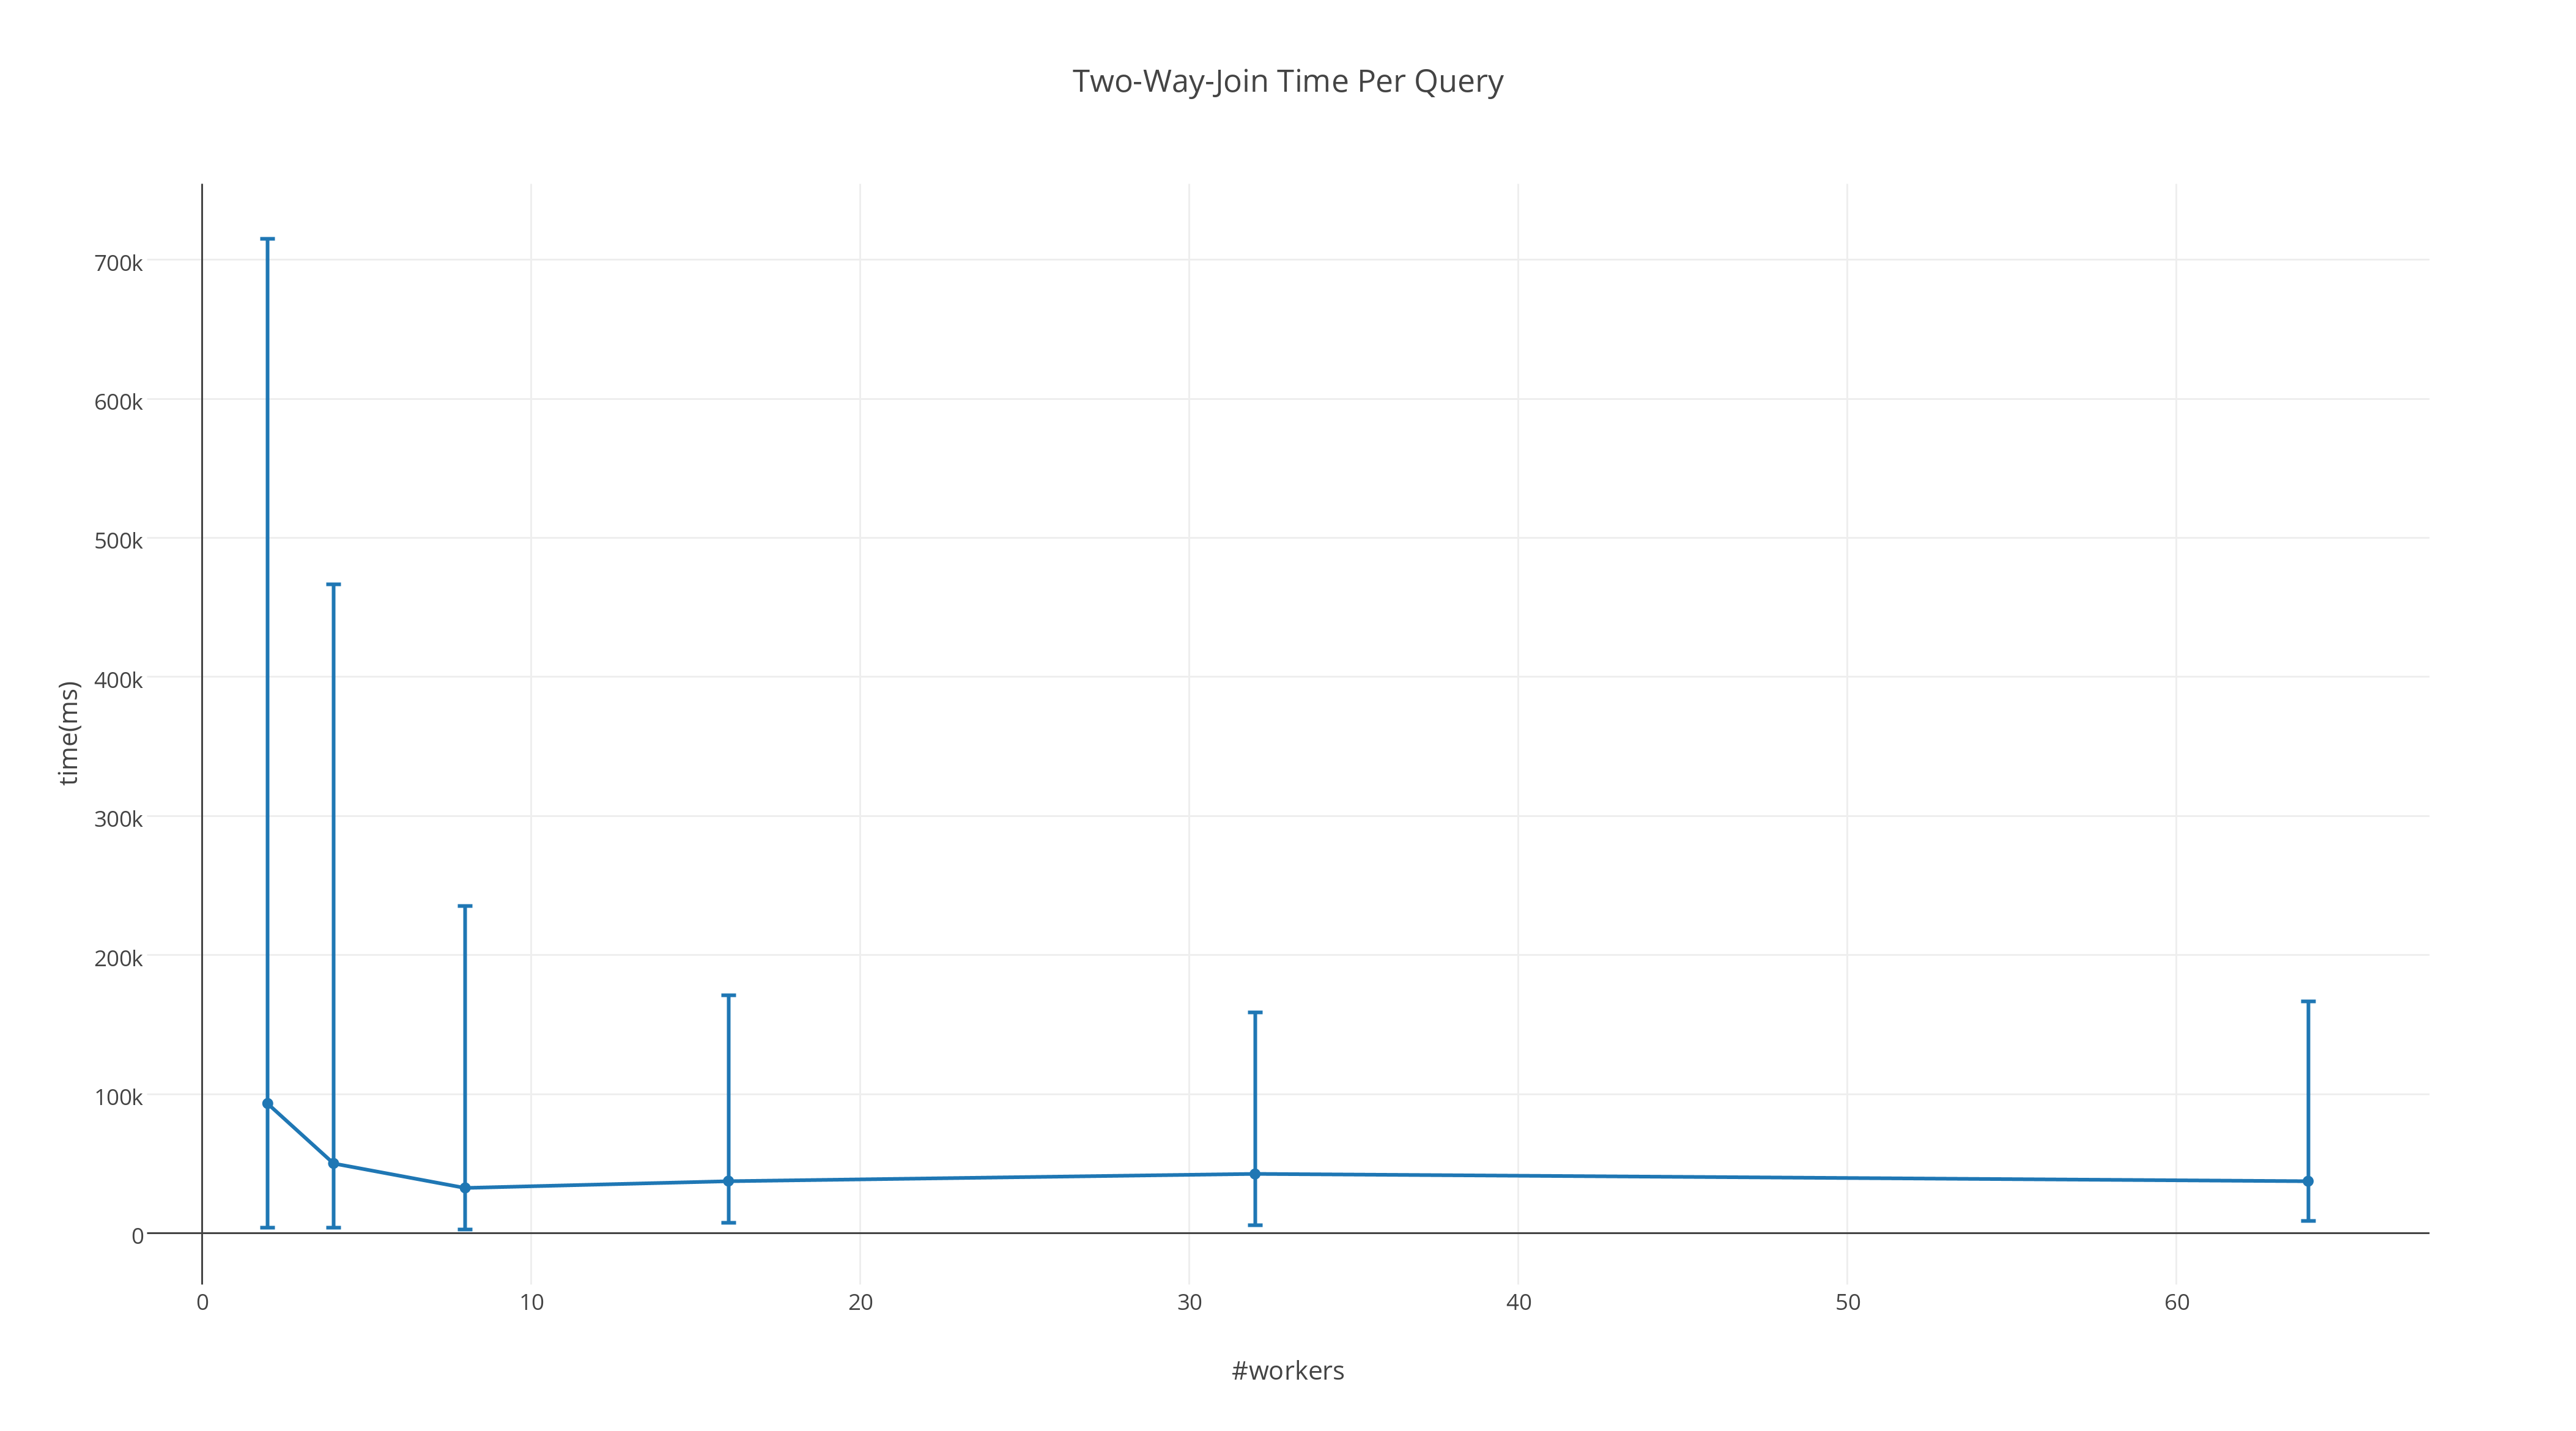
\includegraphics[width=1.0\textwidth]{img/Two-Way-Join-General}
\end{figure}
\begin{figure}[h!]
  \caption{Average Running Time of Multi-Way Join}
  \label{fig:multi-way-general}
  \centering
    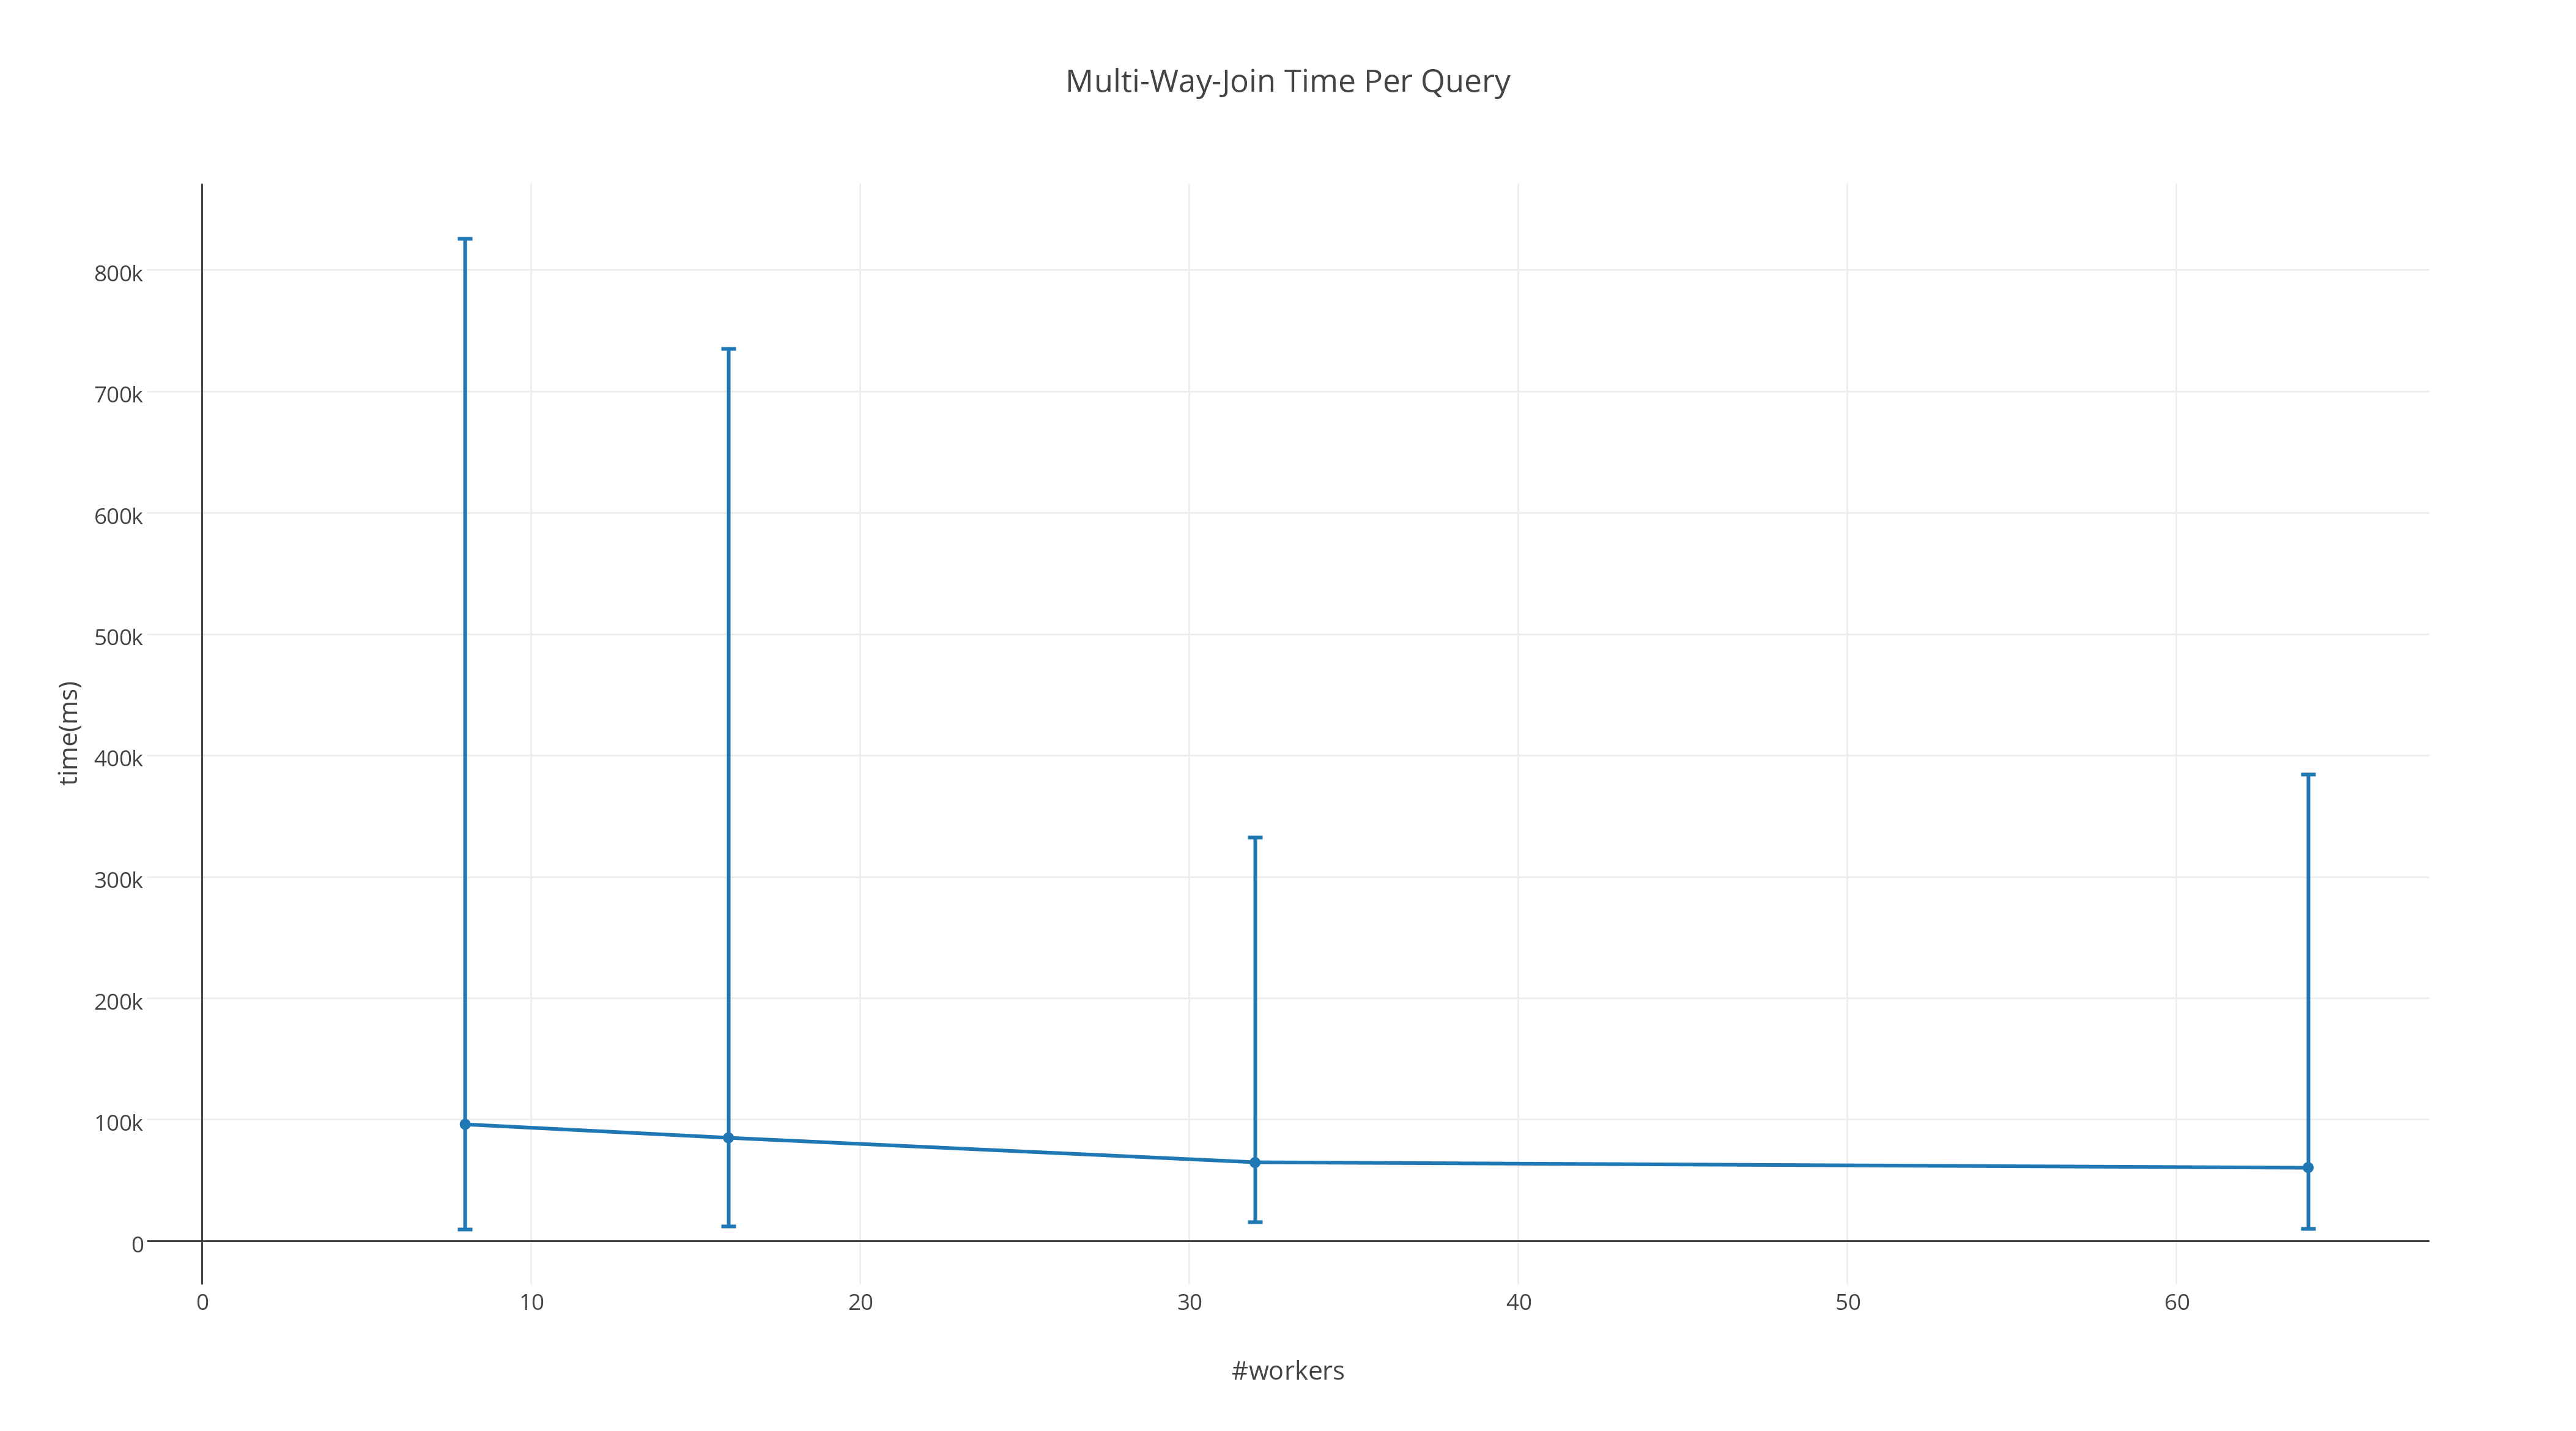
\includegraphics[width=0.8\textwidth]{img/Multi-Way-Join-General}
\end{figure}
\begin{figure}[h!]
  \caption{Average Running Time of Modified Dan Suciu's Algorithm}
  \label{fig:Dan-Algorithm-General}
  \centering
    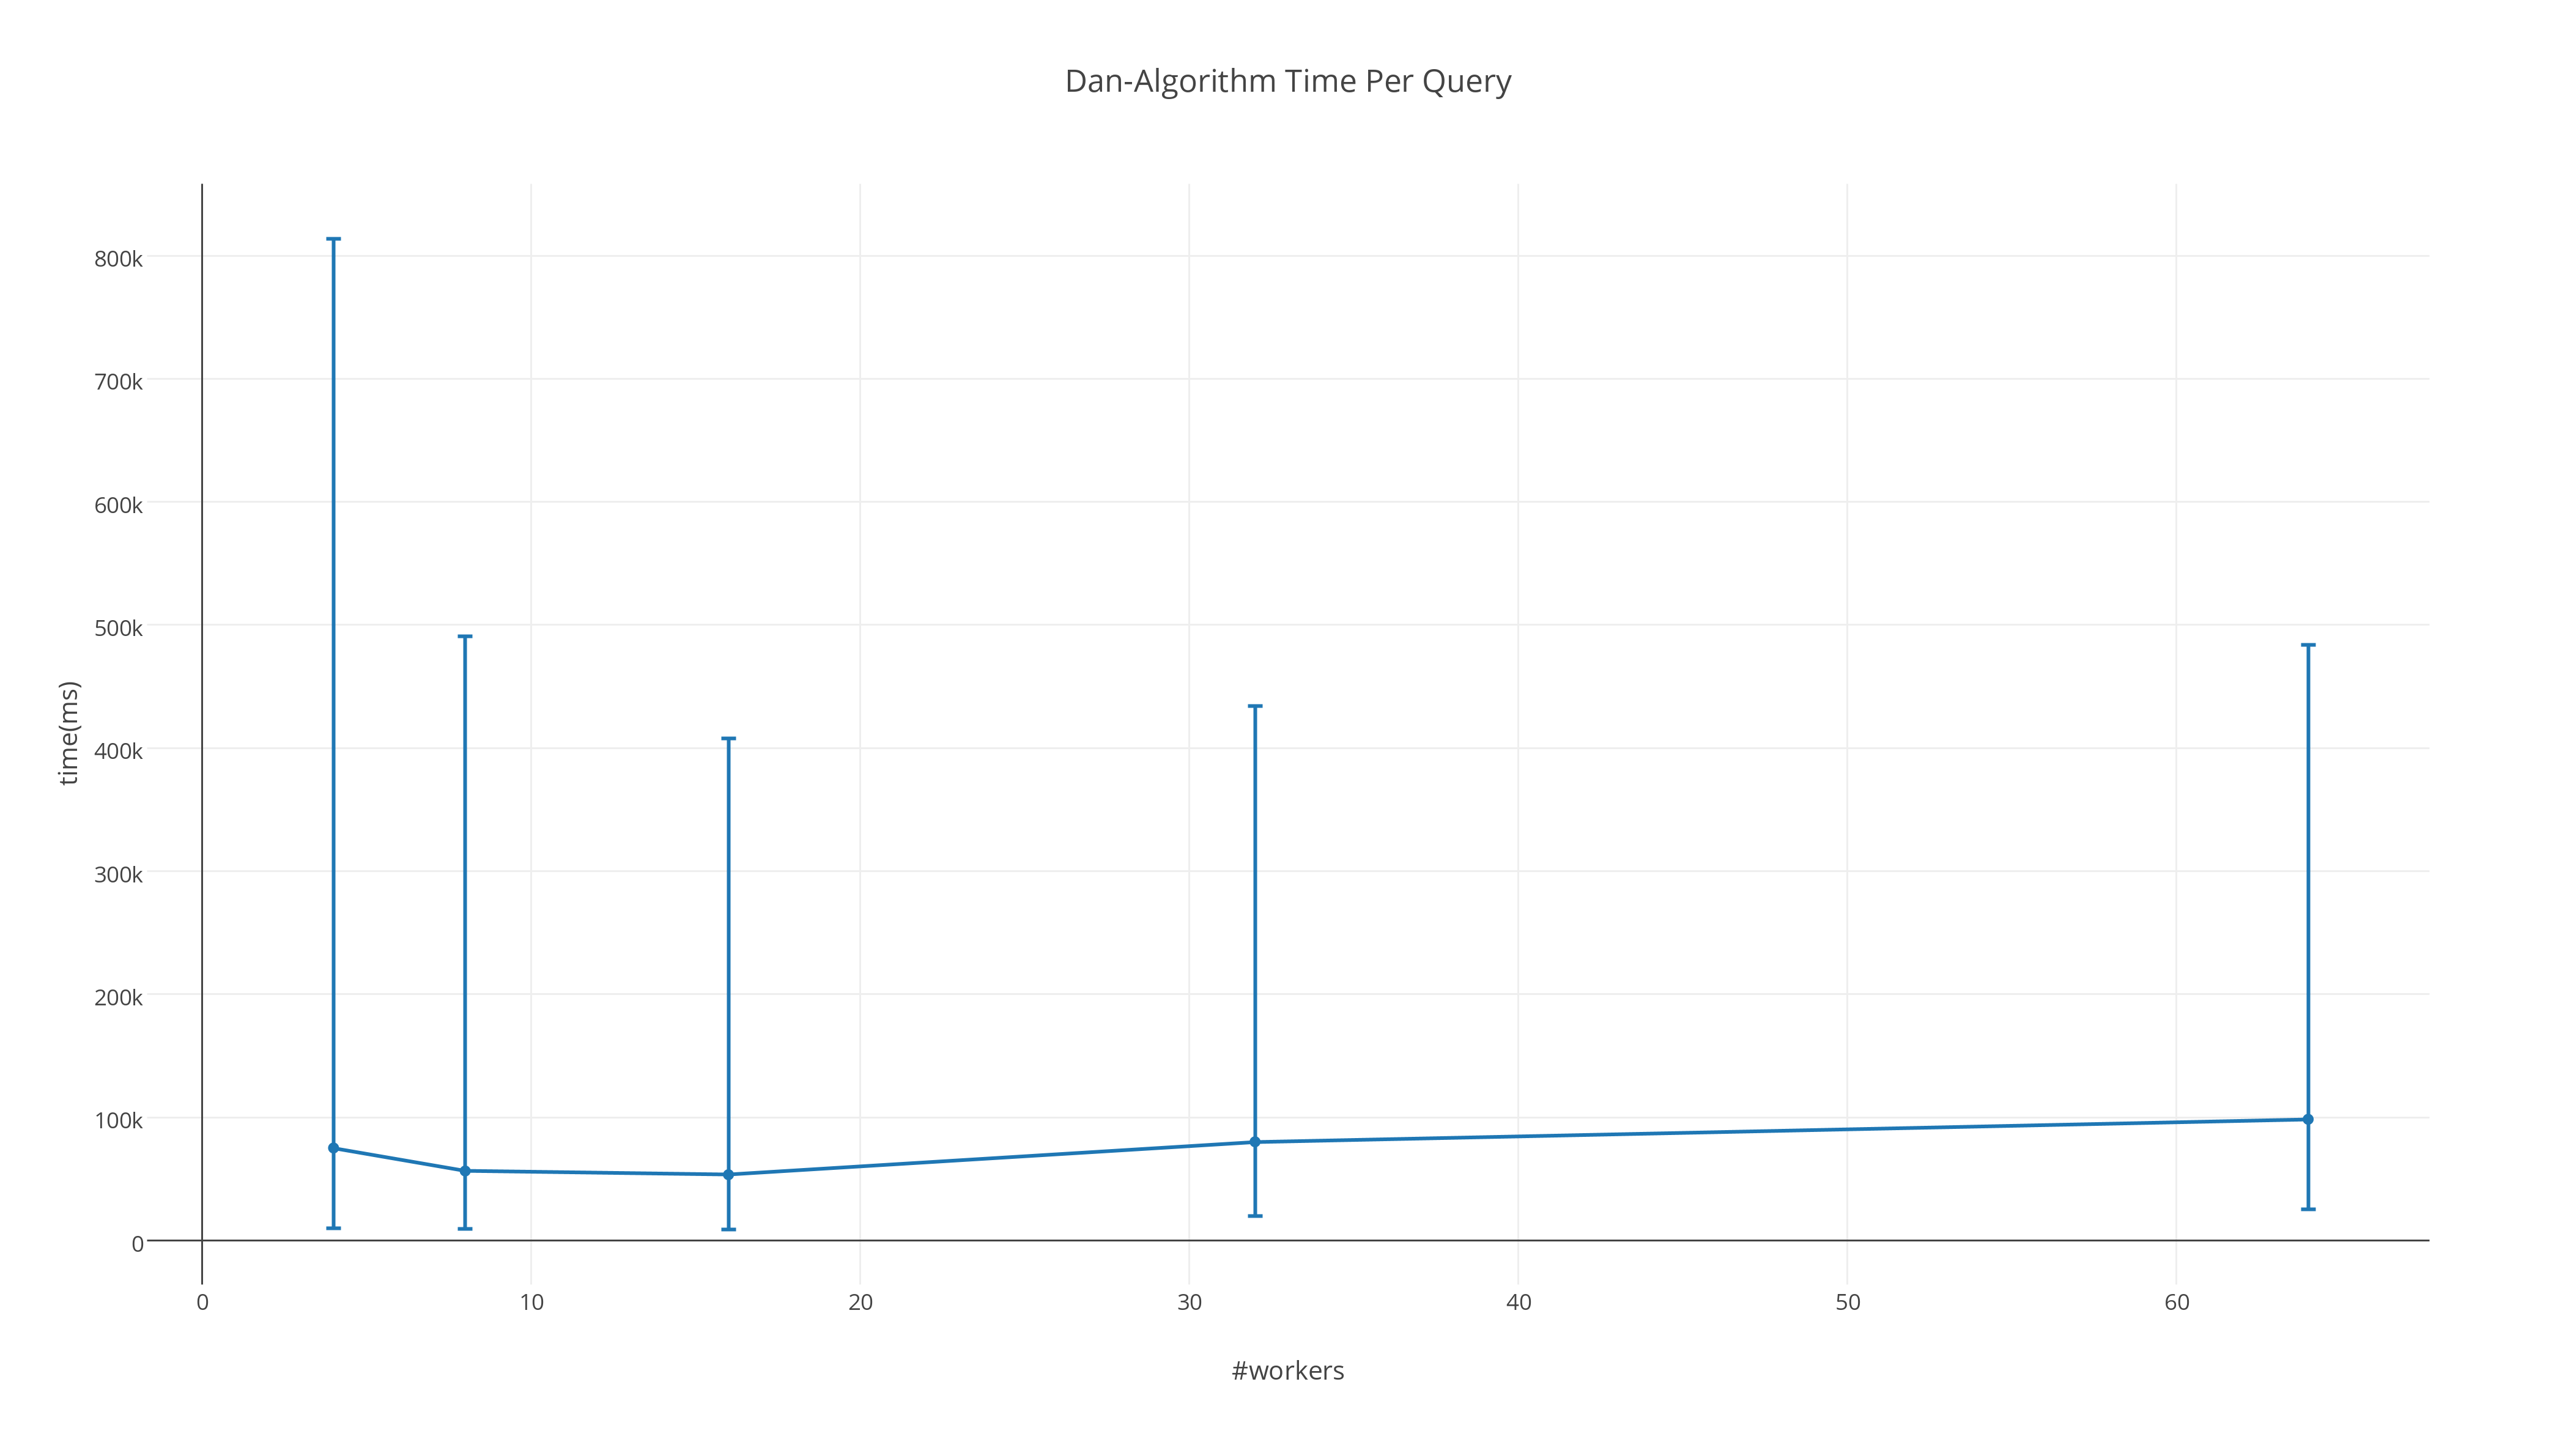
\includegraphics[width=0.8\textwidth]{img/Dan-Algorithm-General}
\end{figure}
\\From the Figure \ref{fig:two-way-join-general} and Figure \ref{fig:multi-way-general} we can see that each query takes around one minute in average. The difference between maximum values of different number of processors indicates that there is a small part of queries which take much longer time. This can be improved significantly by adding more workers. The time spent on a long query is still decreasing with 16 workers while minimum time increases, which in total makes average time higher as there are more simple queries. 
\\Average Running Time for Dan Suciu's algorithm goes up after 16 workers since the graph is split into slight pieces, and there is less chance to do the local search on each partition. In this case, more computation happens on the driver side with more small fragments, which increases the running time. This phenomenon will be discussed further in next chapter.
\\In general, for this data and query size, the running time is already very short, so that introducing more computation power cannot make up with the overhead brought by it. The evidence for this can be found in the next section.
\section{Time Stack}
\begin{figure}[h!]
  \caption{Time Stack of Two-Way Join}
  \label{fig:two-way-join-stack}
  \centering
    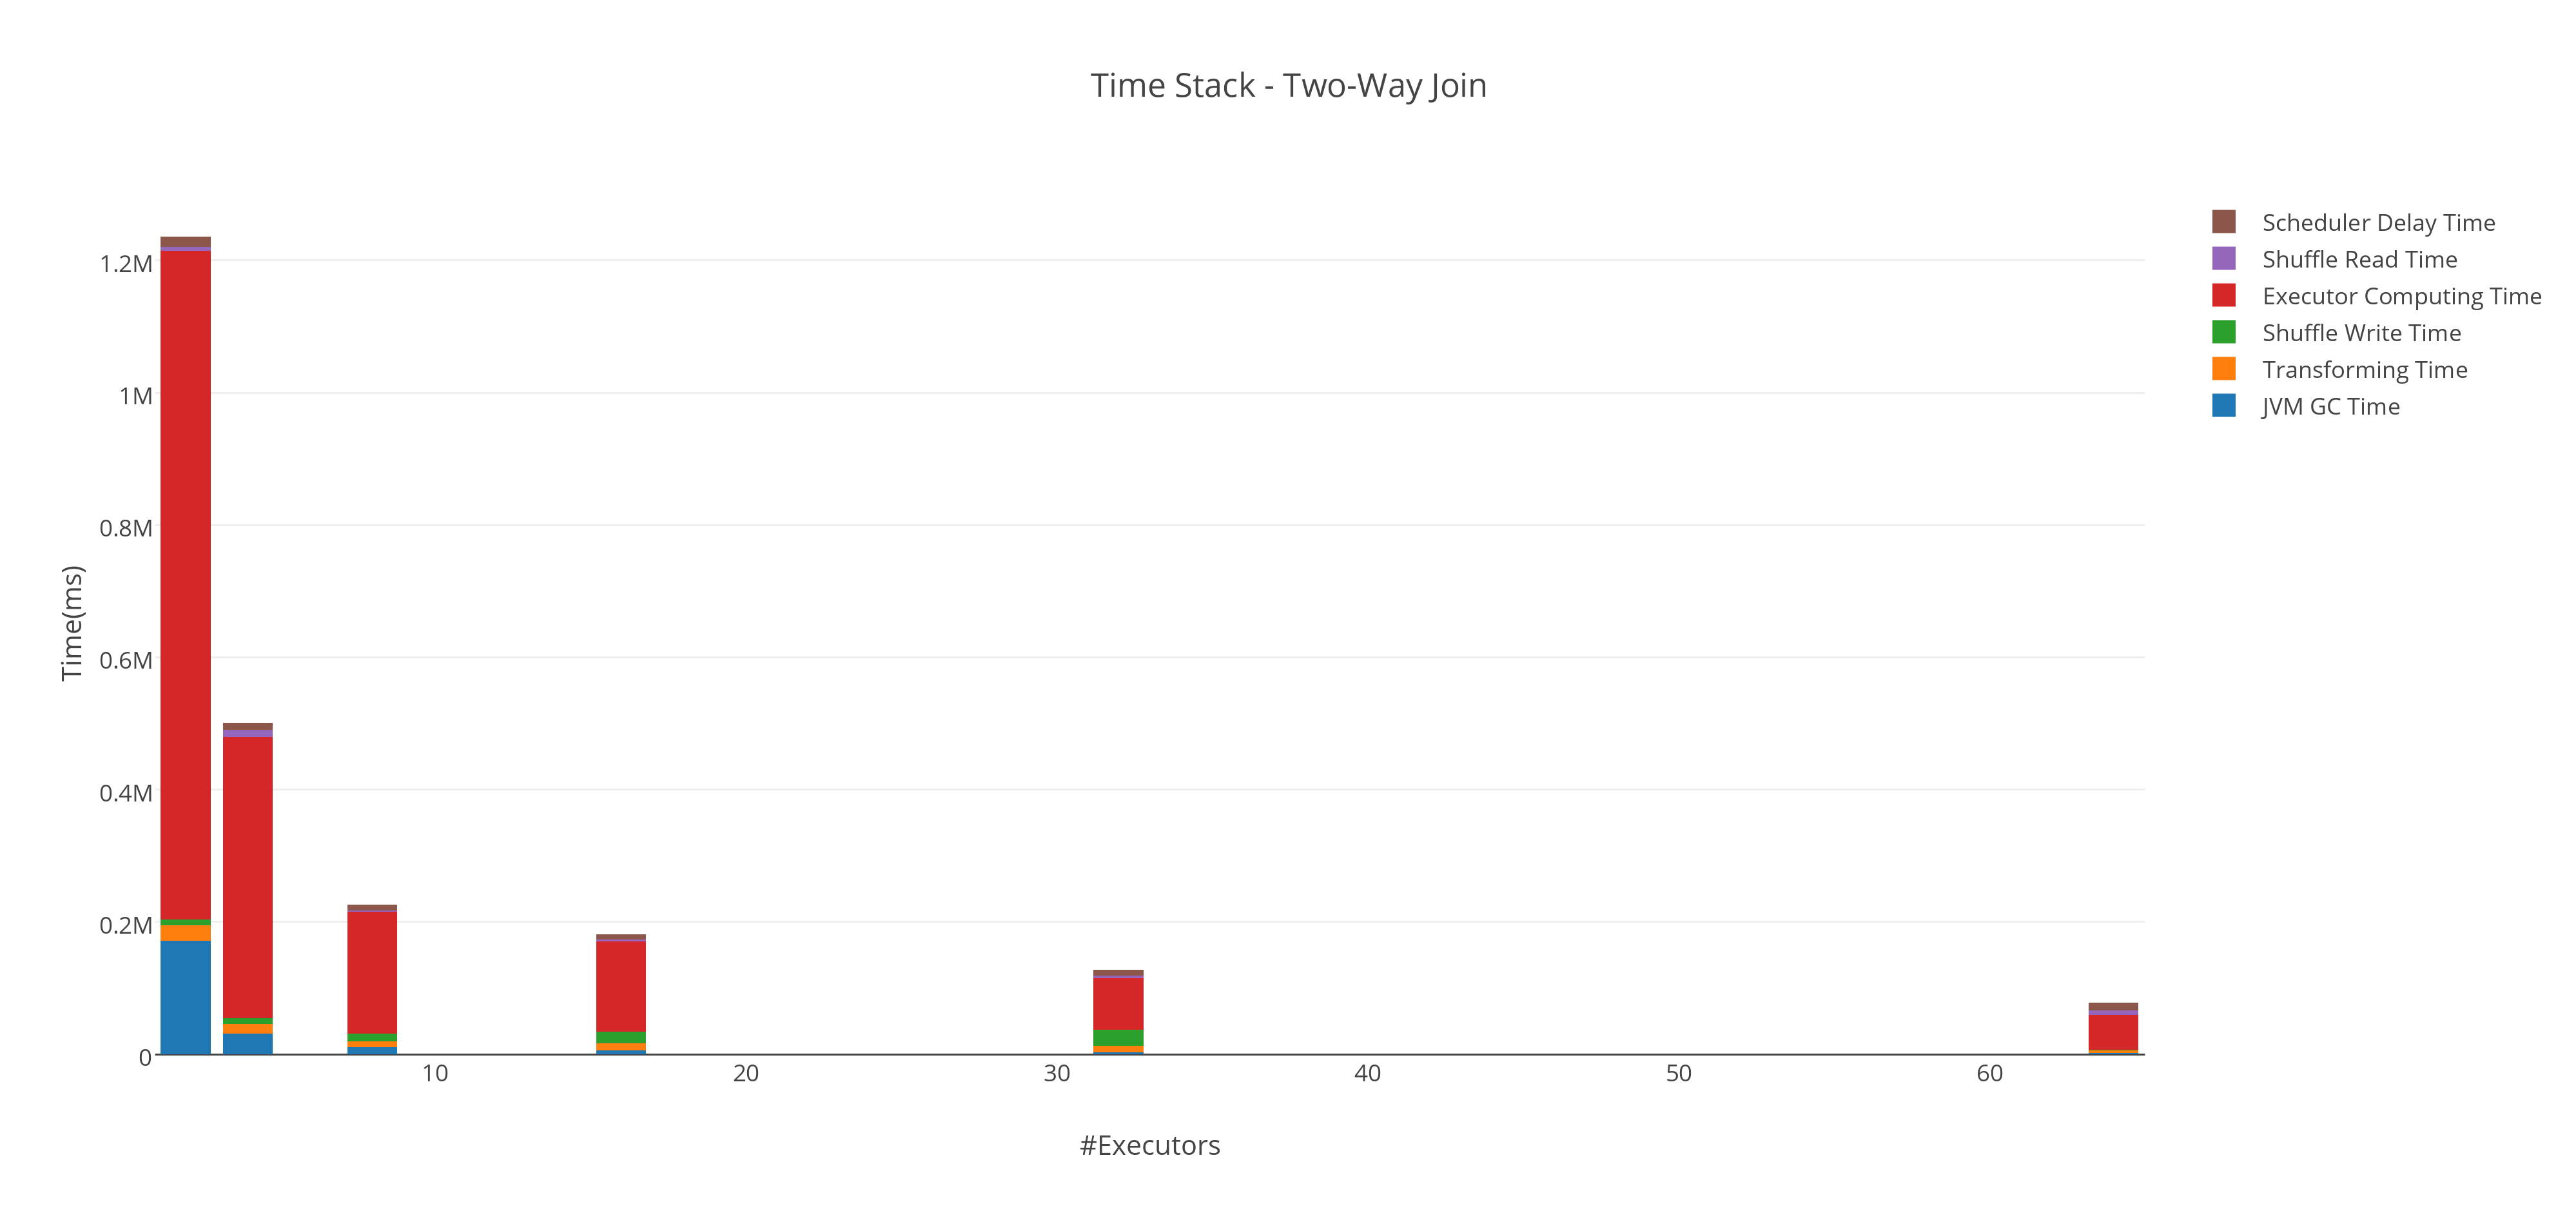
\includegraphics[width=1.0\textwidth]{img/Timestack-twoway}
\end{figure}
\begin{figure}[h!]
  \caption{Time Stack of Multi-Way Join}
  \label{fig:timestack-multiway}
  \centering
    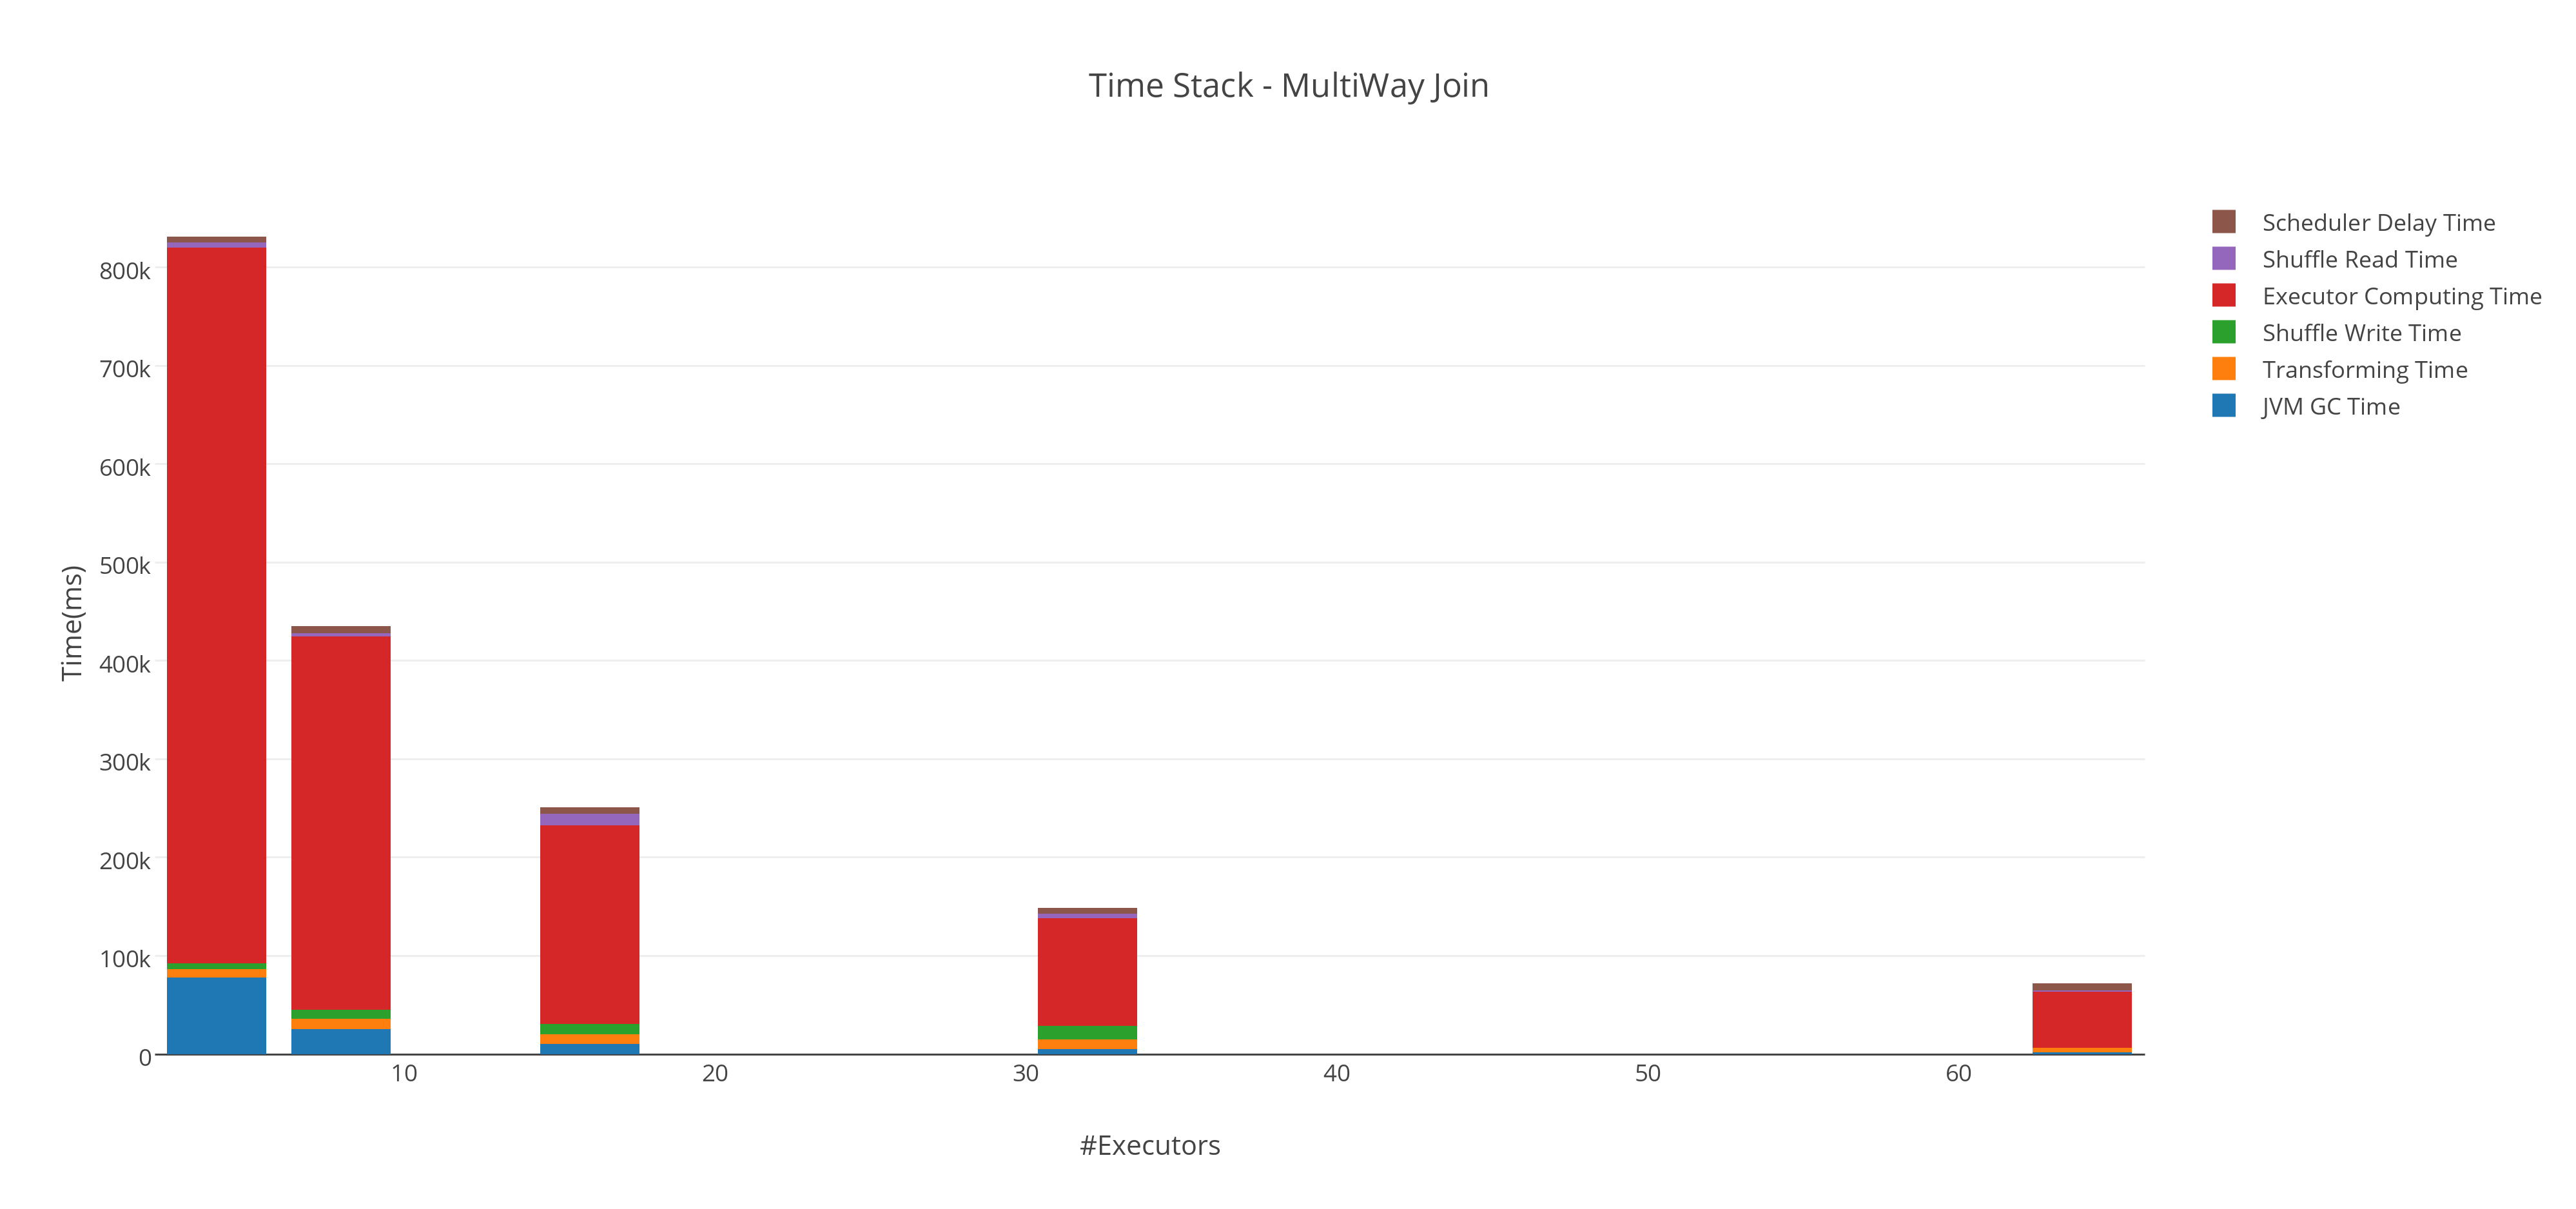
\includegraphics[width=0.8\textwidth]{img/Timestack-multiway}
\end{figure}
According to the diagrams \ref{fig:two-way-join-stack} and \ref{fig:timestack-multiway}, the average executor computing time is always decreasing after adding more workers. Specifically, the time spent on computing is quite small when the number of workers is 64. The reason behind those trends being different from the ones in figure  \ref{fig:two-way-join-general} and figure \ref{fig:multi-way-general} is that tasks are not evenly distributed on different executors, and the blocking time can not be revealed by the average time we measured here. The GC Time is also decreasing dramatically as with more workers as each executor would use less memory. Comparing to the blocking time, the time spent on writing and reading the shuffled data is relatively ignorable, although they are also increasingly slow. The time stack for Dan Scuciu's algorithm is not shown here as the actual running time for each executor is less than $1/10$ of the total time, which will be discussed in bottleneck part.\\
One reason the Multi-way Join is being slower than cascaded two-way join is that the time difference between the busiest executor and idlest one is larger, which is revealed in diagram  \ref{fig:Time-Range-Difference-For-All-Executors.png}. The shuffle phases in the cascaded two-way join are scheduled by native spark function, which can dispatch tasks to processors evenly. However, because of the nature of the Multi-way Join, the size of different reducing tasks in the Multi-way Join can be very different, which explains the phenomenon that some executors are busy while others are just blocked and waiting for them.
\begin{figure}[h!]
  \caption{Maximum Blocking Time for Executors}
  \label{fig:Time-Range-Difference-For-All-Executors.png}
  \centering
    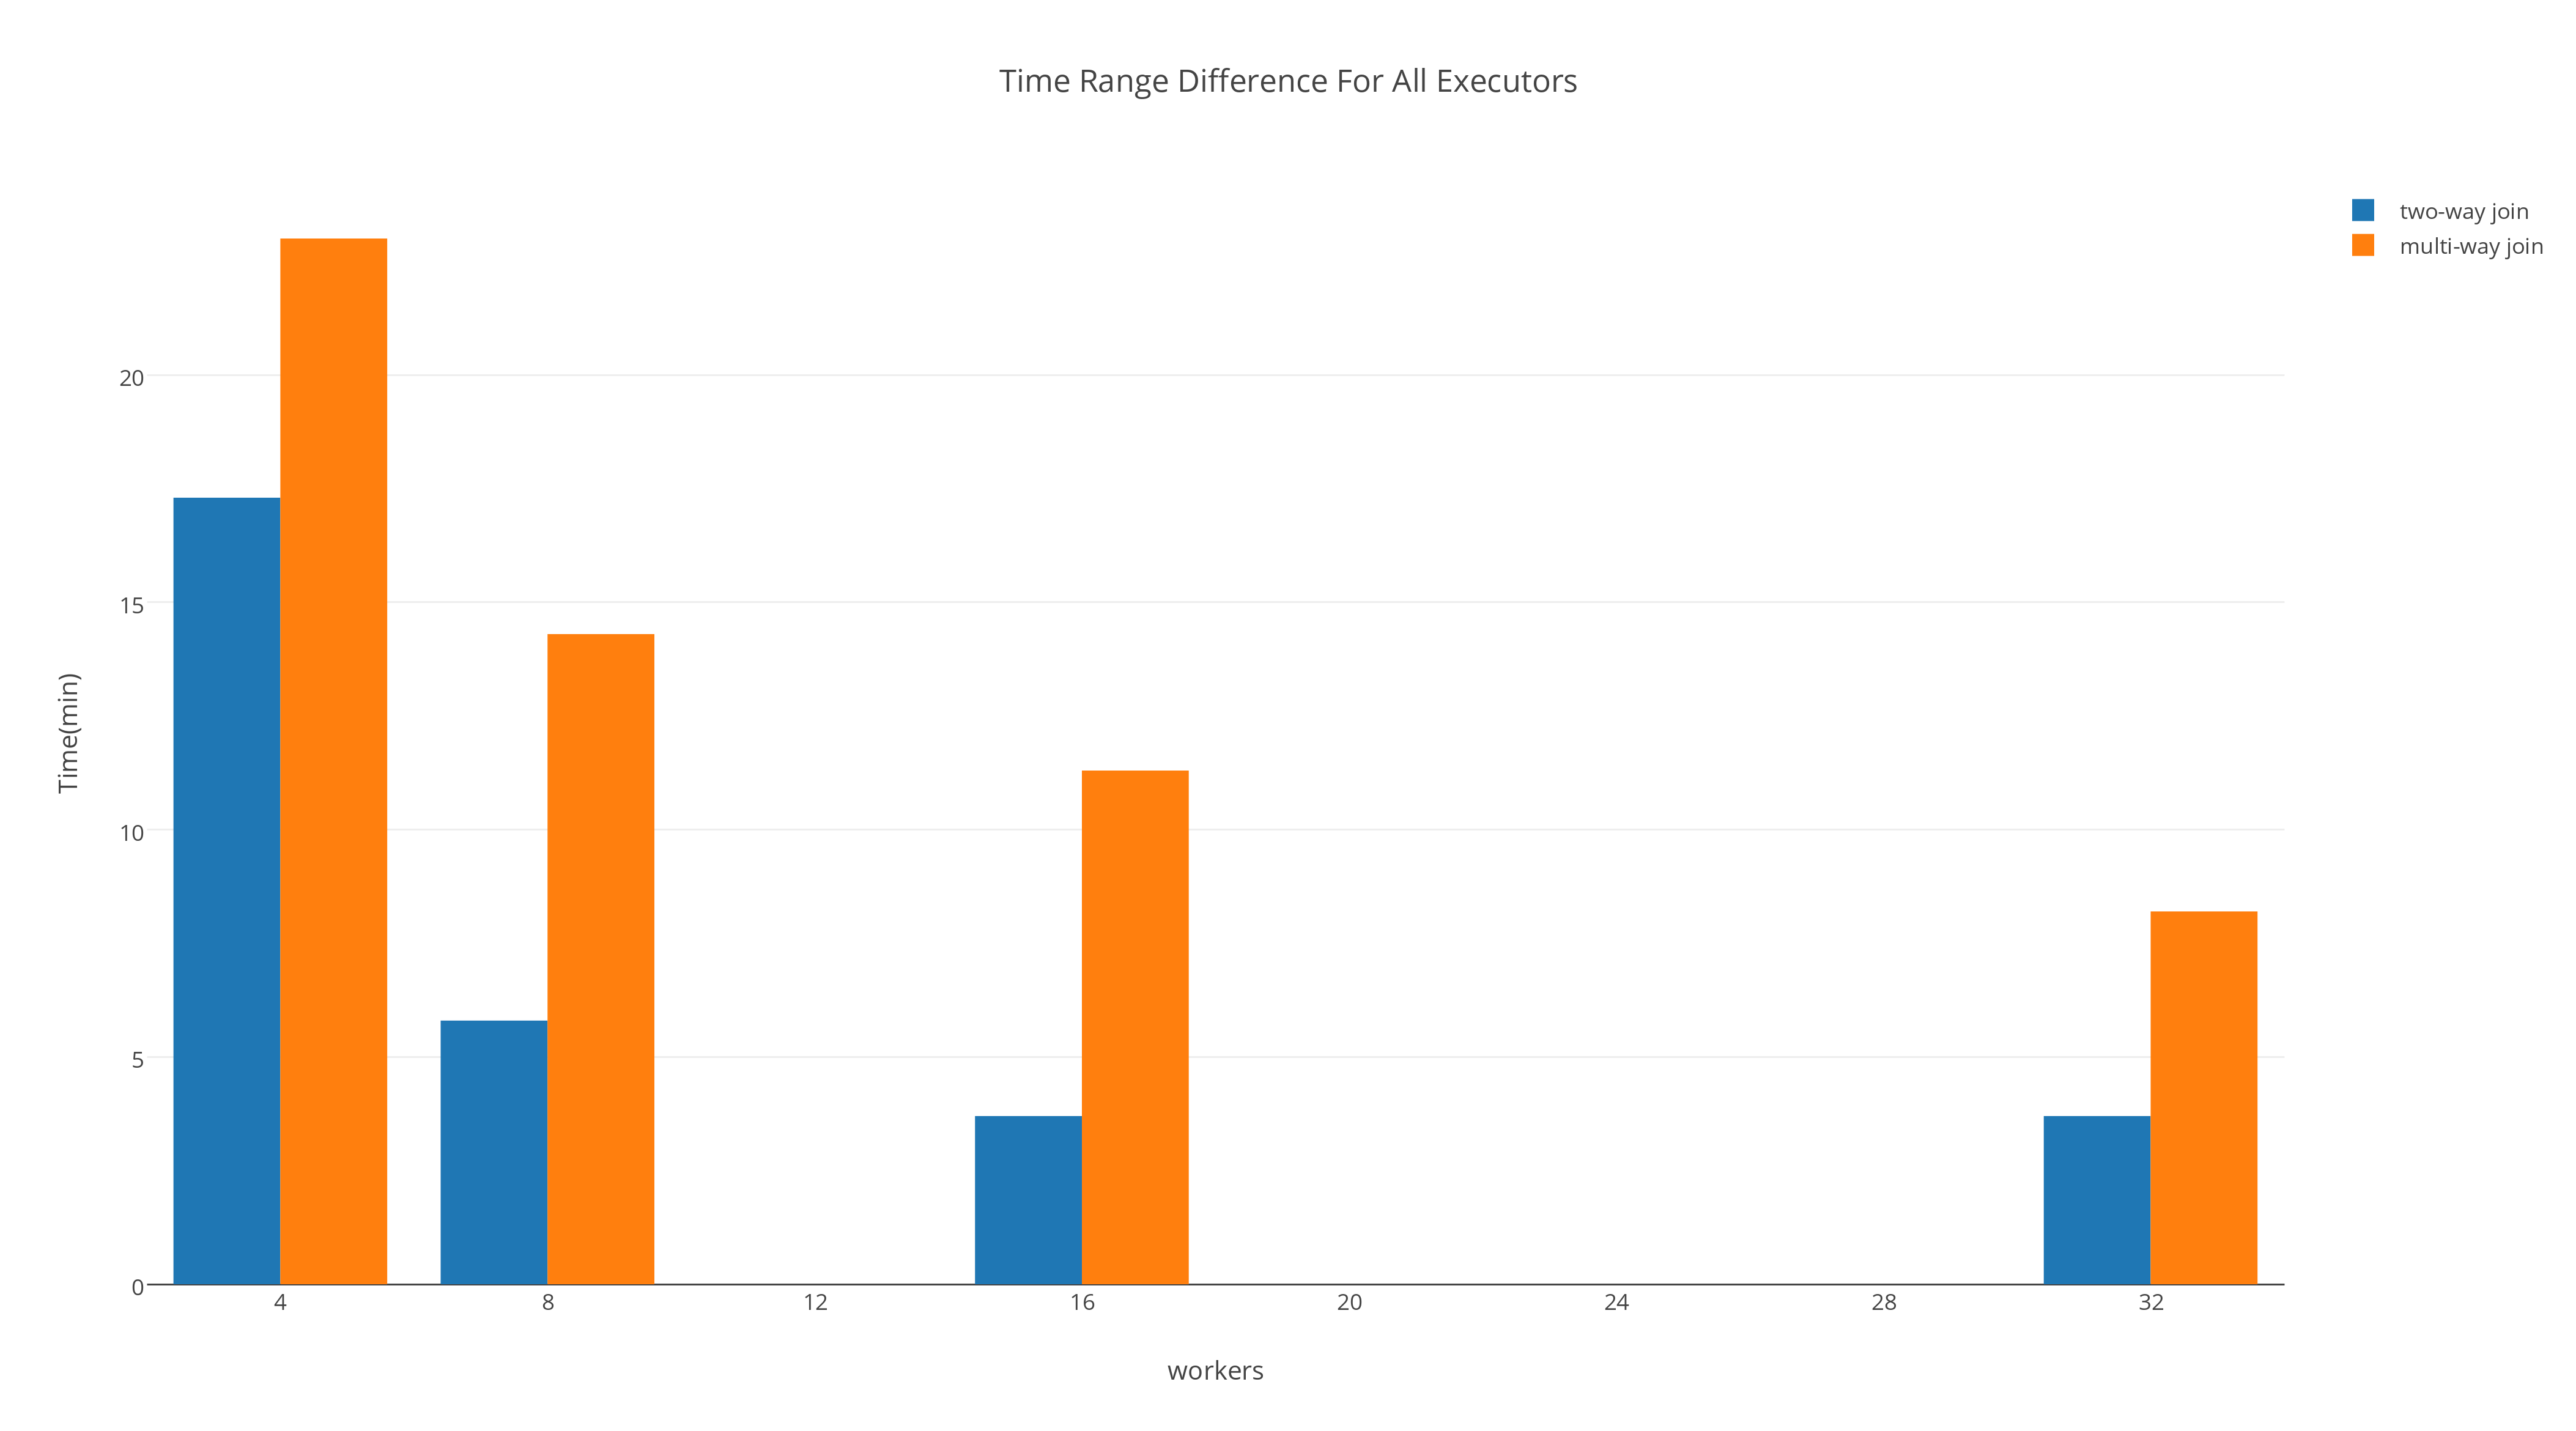
\includegraphics[width=0.8\textwidth]{img/Time-Range-Difference-For-All-Executors}
\end{figure}

\section{Bottleneck}
Furthermore, more insights are revealed by the job flow-chart in Spark Web-UI. The charts  \ref{fig:alibaba-two-jobs}, \ref{fig:alibaba-multi-jobs} and \ref{fig:alibaba-dan-jobs} present the status of different spark jobs along the time-line.
\begin{figure}[h!]
  \caption{Job Flow of Cascaded Two-Way Join}
  \label{fig:alibaba-two-jobs}
  \centering
    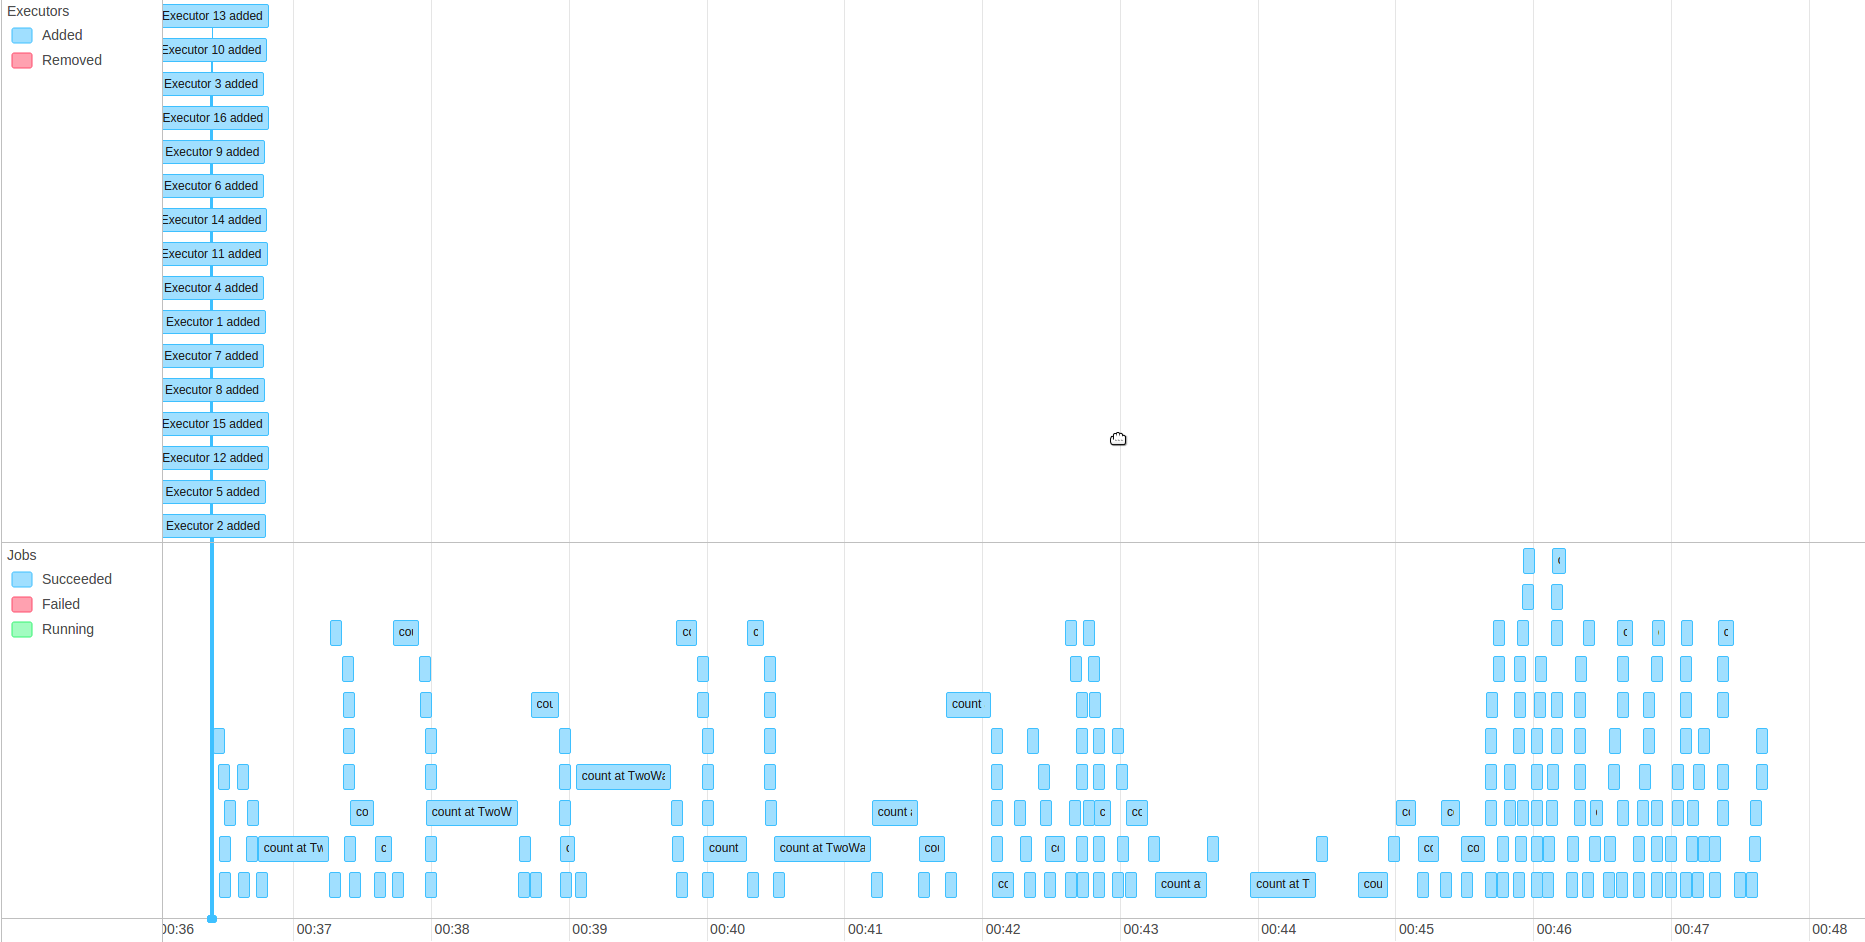
\includegraphics[width=1.0\textwidth]{img/alibaba-two-jobs}
\end{figure}
\begin{figure}[h!]
  \caption{Job Flow of Multi-Way Join}
  \label{fig:alibaba-multi-jobs}
  \centering
    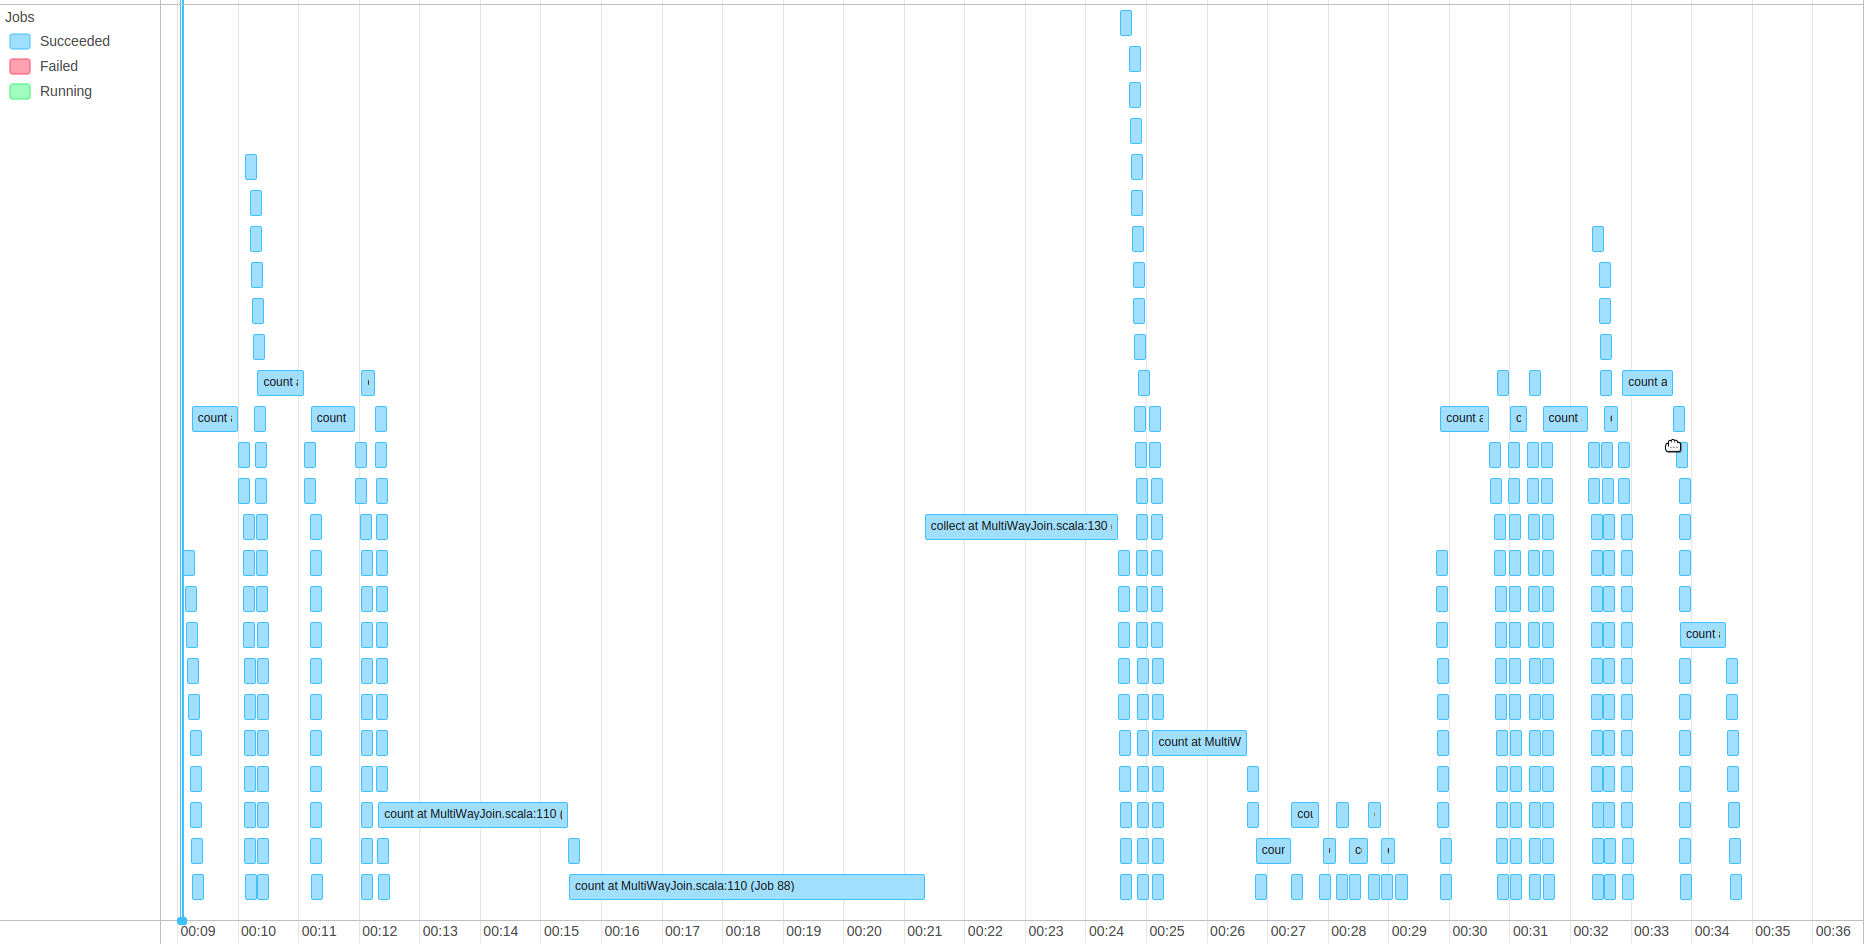
\includegraphics[width=0.8\textwidth]{img/alibaba-multi-jobs}
\end{figure}
\begin{figure}[h!]
  \caption{Job Flow of Modified Dan Suciu's Algorithm}
  \label{fig:alibaba-dan-jobs}
  \centering
    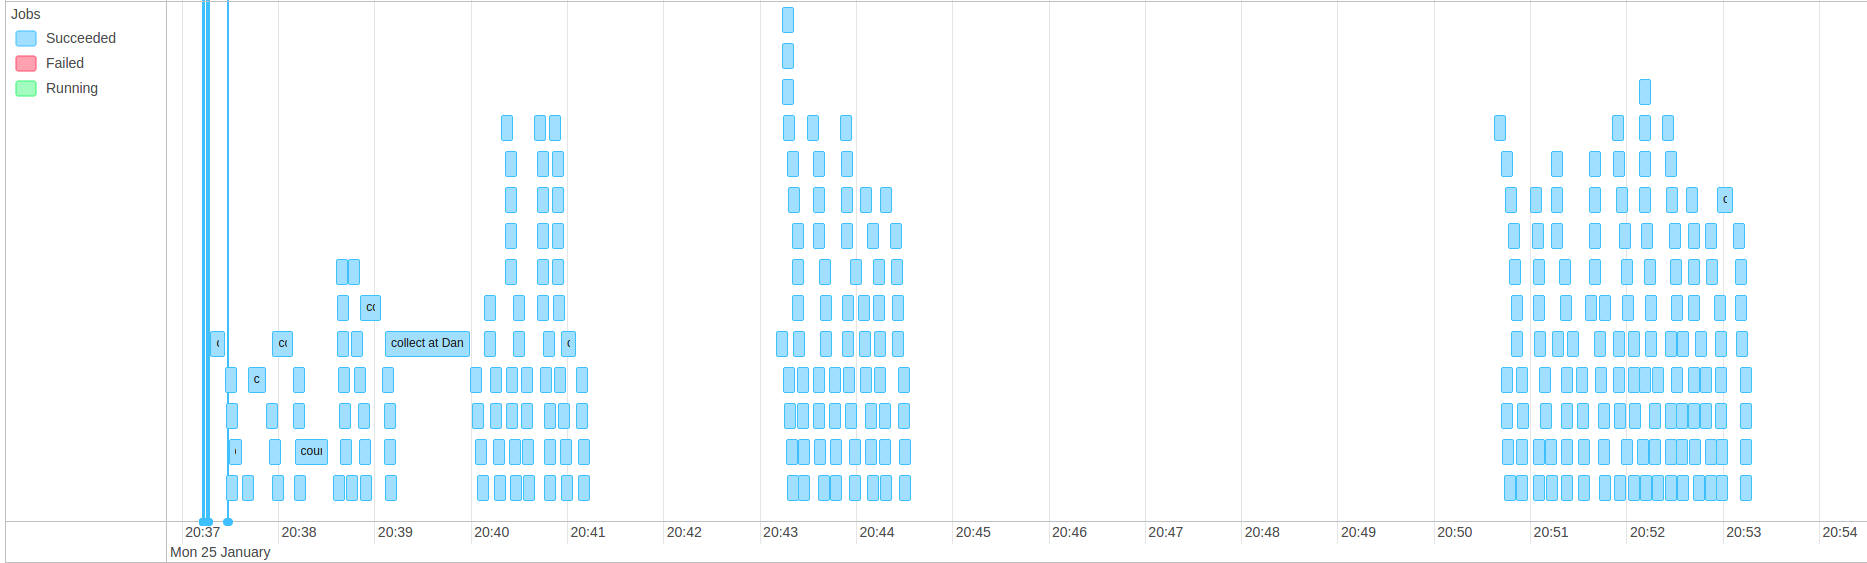
\includegraphics[width=0.8\textwidth]{img/alibaba-dan-jobs}
\end{figure}
\subsubsection{Cascaded 2-way Join}
By comparing those three charts, it can be found that there's no obvious bottleneck in the cascaded two-way join, which proves it to be the most scalable solution under Spark Context. The jobs taking more time are the `count' jobs in process graph \ref{fig:two-way-join-spark}. As Spark is of the lazy-evaluation model, it cannot be concluded that it's the `count'  task that taking so much time. By looking deeper into tasks of the `count' job in figure \ref{fig:alibaba-two-tasks}, it turns out that the full shuffle phases such as `subtract' and `distinct' costs the most time in `count' job. 
\subsubsection{Multi-way Join}
With respect to the Multi-way Join, we can see more obvious bottlenecks of `count' and `collect' jobs. During those jobs, edges distributed to different processors are merged in each task, which could result in huge blocking times as discussed in the previous section.
\begin{figure}[h!]
  \caption{Tasks of Count Job}
  \label{fig:alibaba-two-tasks}
  \centering
    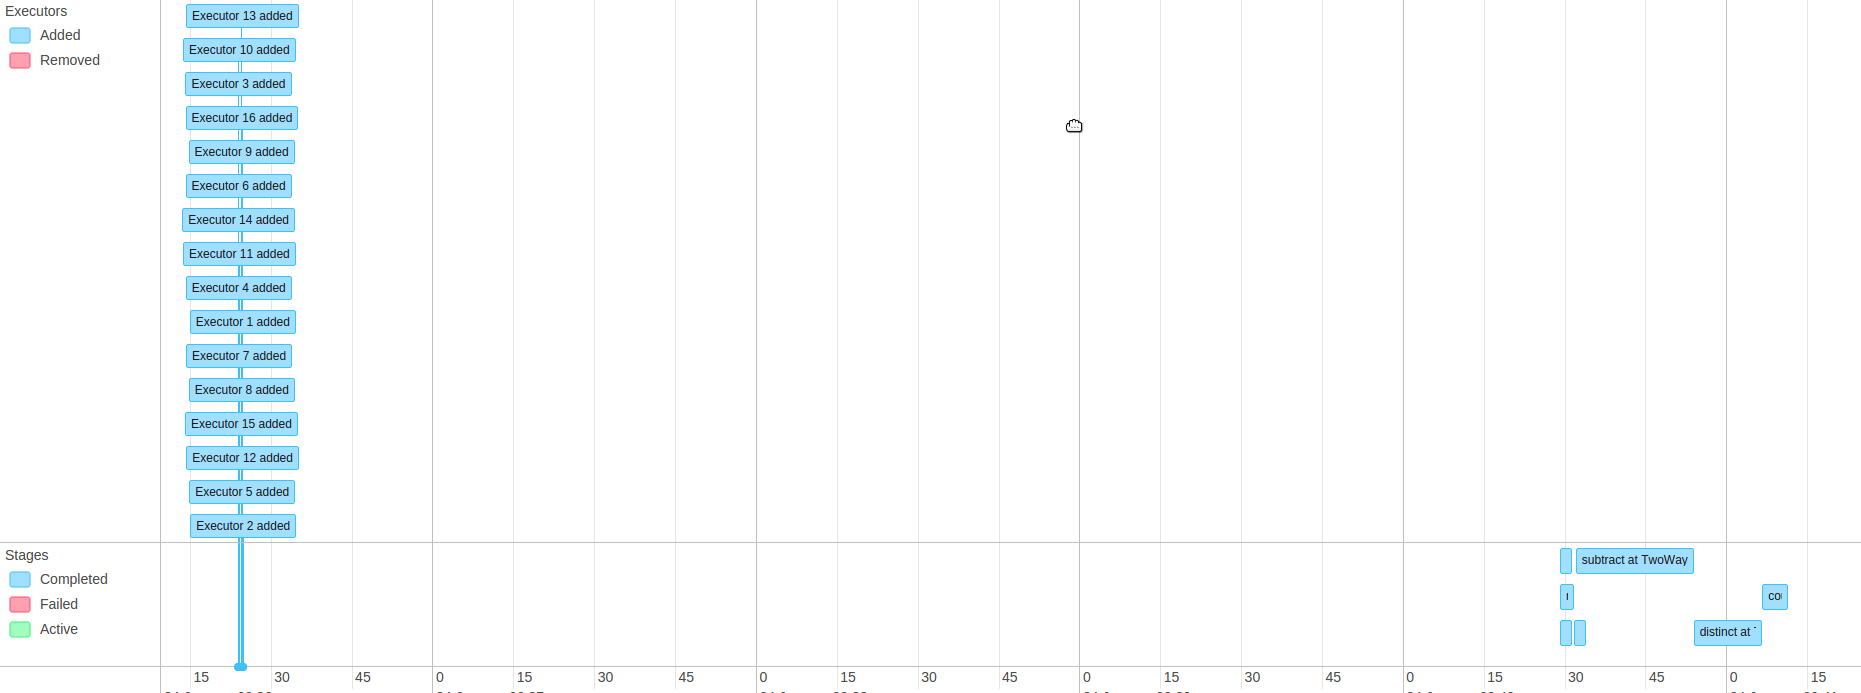
\includegraphics[width=1.0\textwidth]{img/alibaba-two-tasks}
\end{figure}
\subsubsection{Dan Suciu's Algorithm}
The blank parts in the chart of Dan Suciu's algorithm represent the time spent on the driver side. It takes more than half of the total time. On the executors' side, every second there are an almost same number of jobs running at the same time, which indicates the high parallelism. So in the next chapter, we will discuss the optimization of Dan Suciu's algorithm by reducing the size of global accessible graph (GAG) collected to the driver, thus reducing the computation time on the driver side.
\section{Data Shuffle Size}
The relation between the number of executors and shuffle size is included in diagram \ref{fig:two-way-join-shuffle}. As shuffle write size equals the sum of local shuffle read and remote shuffle read, we only show shuffle read data exchanged in it.  When we increase the number of workers, the remote read becomes larger. Finally, in the case of 64 workers, most of the shuffle read happens remotely, which is natural since with more workers added, less data will be local, and the probability of data exchange increases consequently.
\begin{figure}[h!]
  \caption{Shuffle Size of Two-Way Join}
  \label{fig:two-way-join-shuffle}
  \centering
    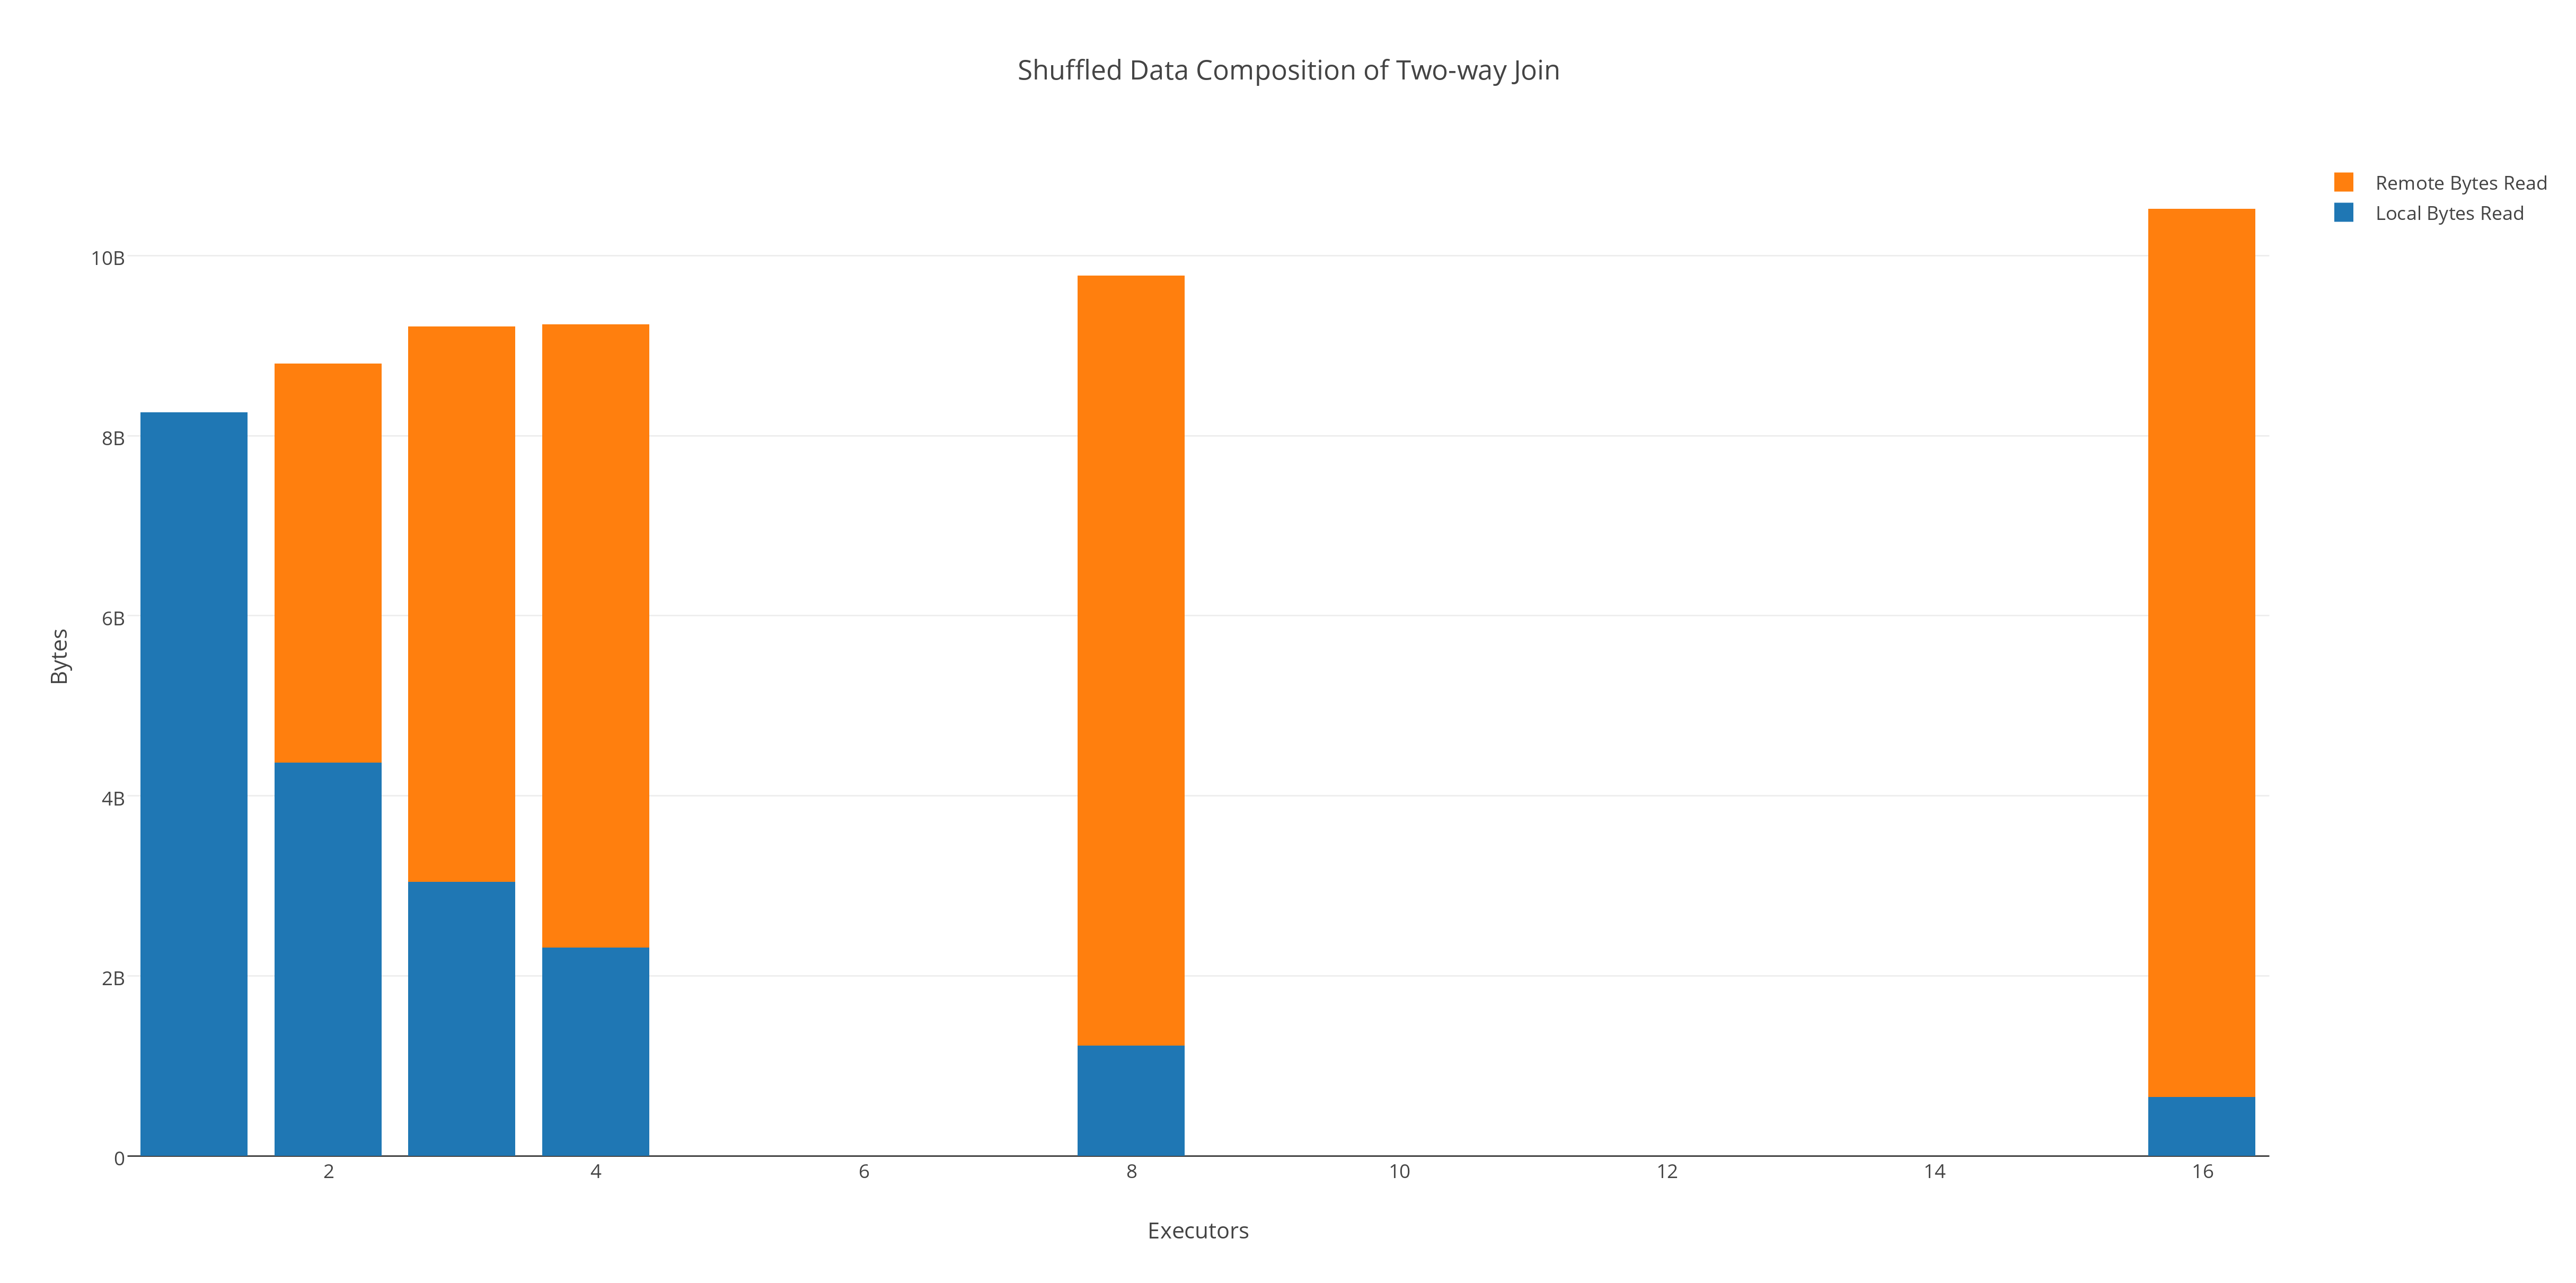
\includegraphics[width=1.0\textwidth]{img/Two-Way-Join-Shuffle-Data}
\end{figure}
\begin{table}[]
\centering
\caption{Shuffle Data Size of 3 Algorithms}
\label{Alibaba-Shuffle-Size}
\begin{tabular}{l|ll|ll|ll|}
   & \multicolumn{2}{c|}{2-way} & \multicolumn{2}{c|}{Multi-way} & \multicolumn{2}{c|}{Dan Scuciu} \\ \cline{2-7} 
   & Local         & Remote        & Local      & Remote      & Local          & Remote         \\ \hline
4  & 1.412 GB        & 5.534 GB        & 2.348 GB      & 7.502 GB        & 87,000 KB               & 252103 KB               \\
8  & 0.916 GB          & 6.182 GB         & 1.360 GB     & 9.273 GB        & 56,842 KB              & 374,842 KB              \\
16 & 0.424 GB          & 7.025 GB         & 0.623 GB       & 10.209 GB       & 37,341 KB              & 578,899 KB              \\
32 & 0.239 GB          & 7.903 GB         & 0.562 GB       & 10.767 GB       & 31,435 KB              & 955,104 KB             
\end{tabular}
\end{table}
\\Figure \ref{Alibaba-Shuffle-Size} compares the total data shuffled size for different algorithms. Comparing to other two algorithms, the shuffle size of Dan Suciu's algorithm can almost be ignored. Although multi-way join only shuffles once and process the local reduce task then, it still shuffles more bytes than cascaded two-way join.
\\However, if we look into more details in shuffle size of all tasks, the following findings can explain why multi-way join didn't improve the shuffle size:
\begin{enumerate}
    \item In the top 10 tasks of Cascaded 2-way Join that shuffle write most bytes, the executors only shuffle 700MB at most and those of the other tasks are around 300MBs. All of them are full shuffle tasks like `subtract' or `distinct'.
    \item With regards to the top 10 tasks of Multi-way Join that shuffle write most bytes, one of them shuffles 4GB , which is almost half of the whole shuffle write volume. And this task is `subtract' task, which is only triggered when dealing with queries with recurrence. This means the Multi-way Join shuffles much more than cascaded 2-way in the extreme case. Besides, all tasks that shuffle more than 100MB are relevant to the `subtract' or `distinct' operation when there is recurrence in the query.
    \item None of those tasks which dispatches states to Reduce tasks costs more than 100MB.
\end{enumerate}
The phenomenon is irrelevant to the number of workers as those bottleneck tasks are all full shuffle phases, which transmit the almost same amount of data despite the number of executors.
% \section{Memory Usage}
% As a trade-off, the multi-way join uses less memory as it doesn't need to cache intermediate results between iterations like cascaded two-way join. The peak memory usage of the two algorithms can be found in table \ref{peak-memory}
% \begin{table}[h!]
% \centering
% \caption{Peak Memory Usage of 2-way and Multi-way Join}
% \label{peak-memory}
% \begin{tabular}{lll}
% executors & cascaded two-way join & multi-way join \\
% 4         & 10.6 GB               & 6.8 GB         \\
% 8         & 19.9GB                & 7.5 GB         \\
% 16        & 27.5GB                & 8.2 GB         \\
% 32        & 32.2GB                & 8.7GB         
% \end{tabular}
% \end{table}

\section{Summary}
In this chapter, we run the Cascaded 2-way Join, Multi-way Join and modified Dan Suciu's algorithm against the Alibaba Benchmark and seek for some interesting findings. The measurements are conducted for metrics including running time, time stack and shuffle size. The following is the summary of observations:
\begin{enumerate}
    \item Cascaded 2-way Join is the most scalable solution of the three algorithms as the tasks are evenly distributed, and executors are blocked for the least time.
    \item Multi-way Join reduces shuffled size for simple queries. However, the shuffle size grows super fast when it deals with a query that contains recurrence.
    \item Dan Suciu's Algorithm seldom conducts shuffle, and it's limited by driver computation.
\end{enumerate}\chapter{\label{cha:par-str}Partition Strategies}
\section{Motivation}
To optimize the performance of Dan Suciu's algorithm, multiple tests were done as described in preceding chapters. The graph was partitioned by default rules, which means that if there are four partitions and 100 nodes, we put node 1-25 into the first partition, 26-50 into the second partition, etc. An interesting finding is that for most queries, the Step 2 in the modified Dan Suciu's Algorithm only runs for one iteration, which indicates all paths in Global Accessible Graph (GAG) collected are of length 1. This reflects that every site only filters all edges that can be part of the result and returns them immediately without doing any local search. The reason behind this is that with a bad partitioner, the search process can easily reach the output node and stop searching. By using a smart partitioner, the distributed search processes run much more iterations, and the size of the GAG is reduced significantly. Thus in this chapter, we firstly observe the relationship between number of input-nodes or cross-edges and the GAG size, then give the theoretical size of GAG in the form of input-nodes number. In the evaluation section, we verify the formulas by running modified Dan Suciu's algorithm against GMark Benchmark graphs which are partitioned by different partitioners.
\section{Observations}
In figure \ref{fig:alibaba-Random-Queries}, we show the testing result for eight random queries from Alibaba benchmark. The application is run with three partitioners: random partitioner, default (ordered) partitioner and METIS partitioner. We choose the GAG size as primary observation target since it's the only data transmitted in theory, affecting network communication as well as computation time.  
\begin{figure}[h!]
  \caption{GAG Size of Random Queries}
  \label{fig:alibaba-Random-Queries}
  \centering
    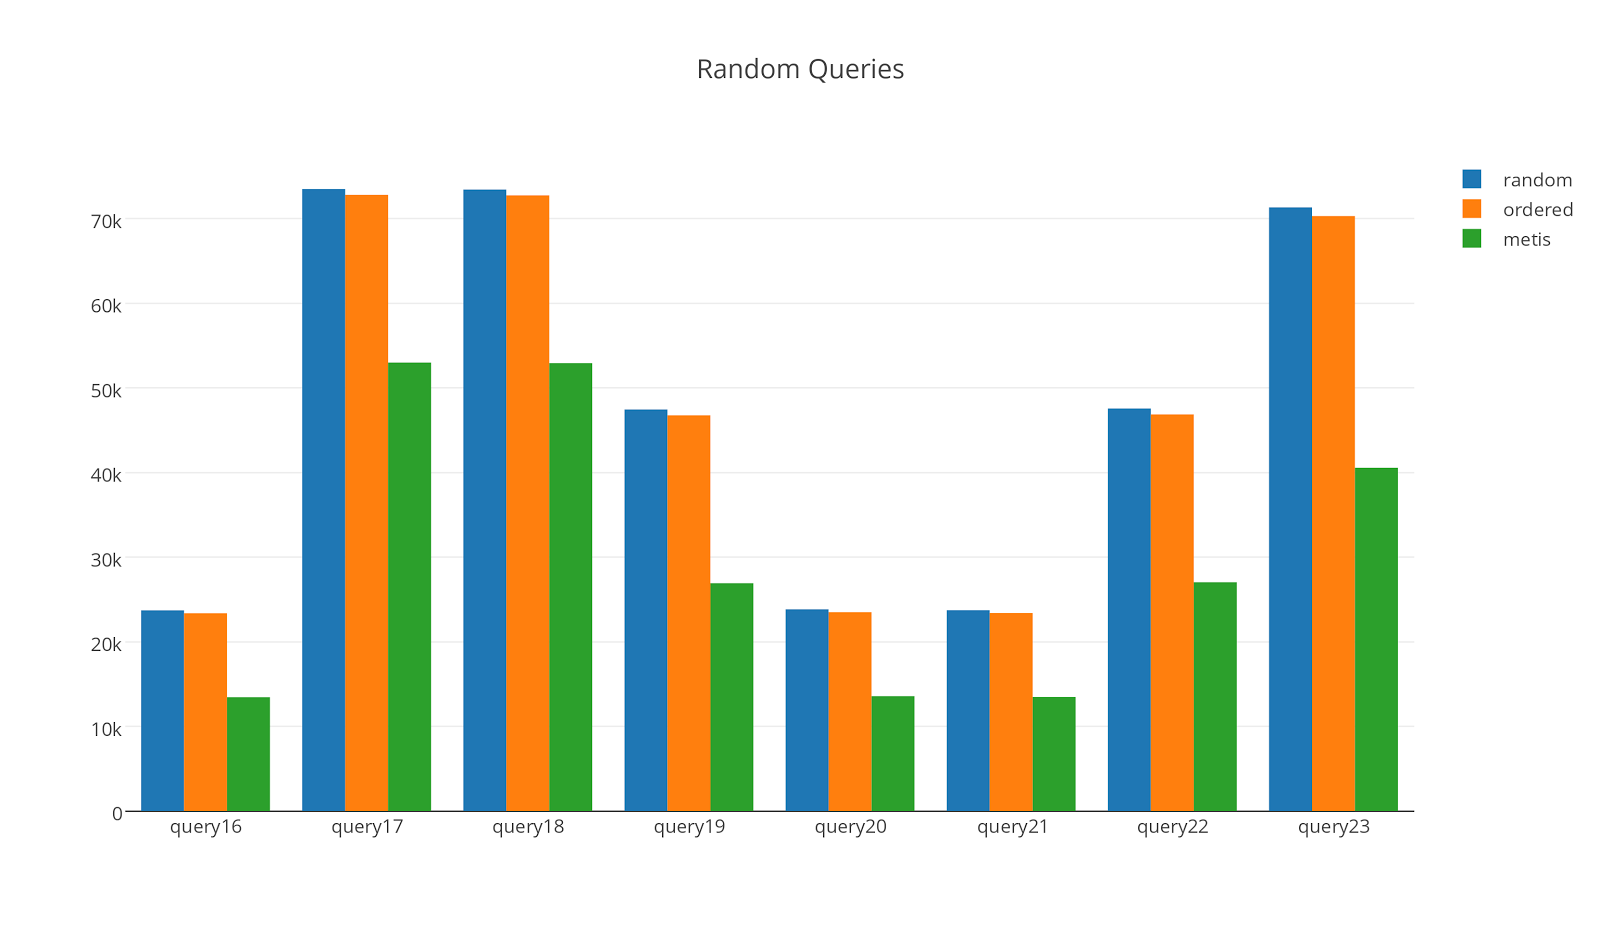
\includegraphics[width=0.8\textwidth]{img/alibaba-Random-Queries}
\end{figure}
\\It turns out that the METIS partitioner can reduce the size of GAG by $30\%-50\%$ comparing to other two partitioners. As mentioned in research background, the METIS algorithm intends to minimize the number of cross-edges while here it turns out that the size of the GAG is not correlated to cross-edges, but the number of input-nodes: In Figure \ref{fig:alibaba-structure}, we can see METIS is not better than the default partitioner in the number of cross-edges, but halves the number of input-nodes. Moreover, the ordered partitioner has much fewer cross-edges than the random partitioner, but still produces a similar size of GAG.
\begin{figure}[h!]
  \caption{Basic Stats for Different Parititioners}
  \label{fig:alibaba-structure}
  \centering
    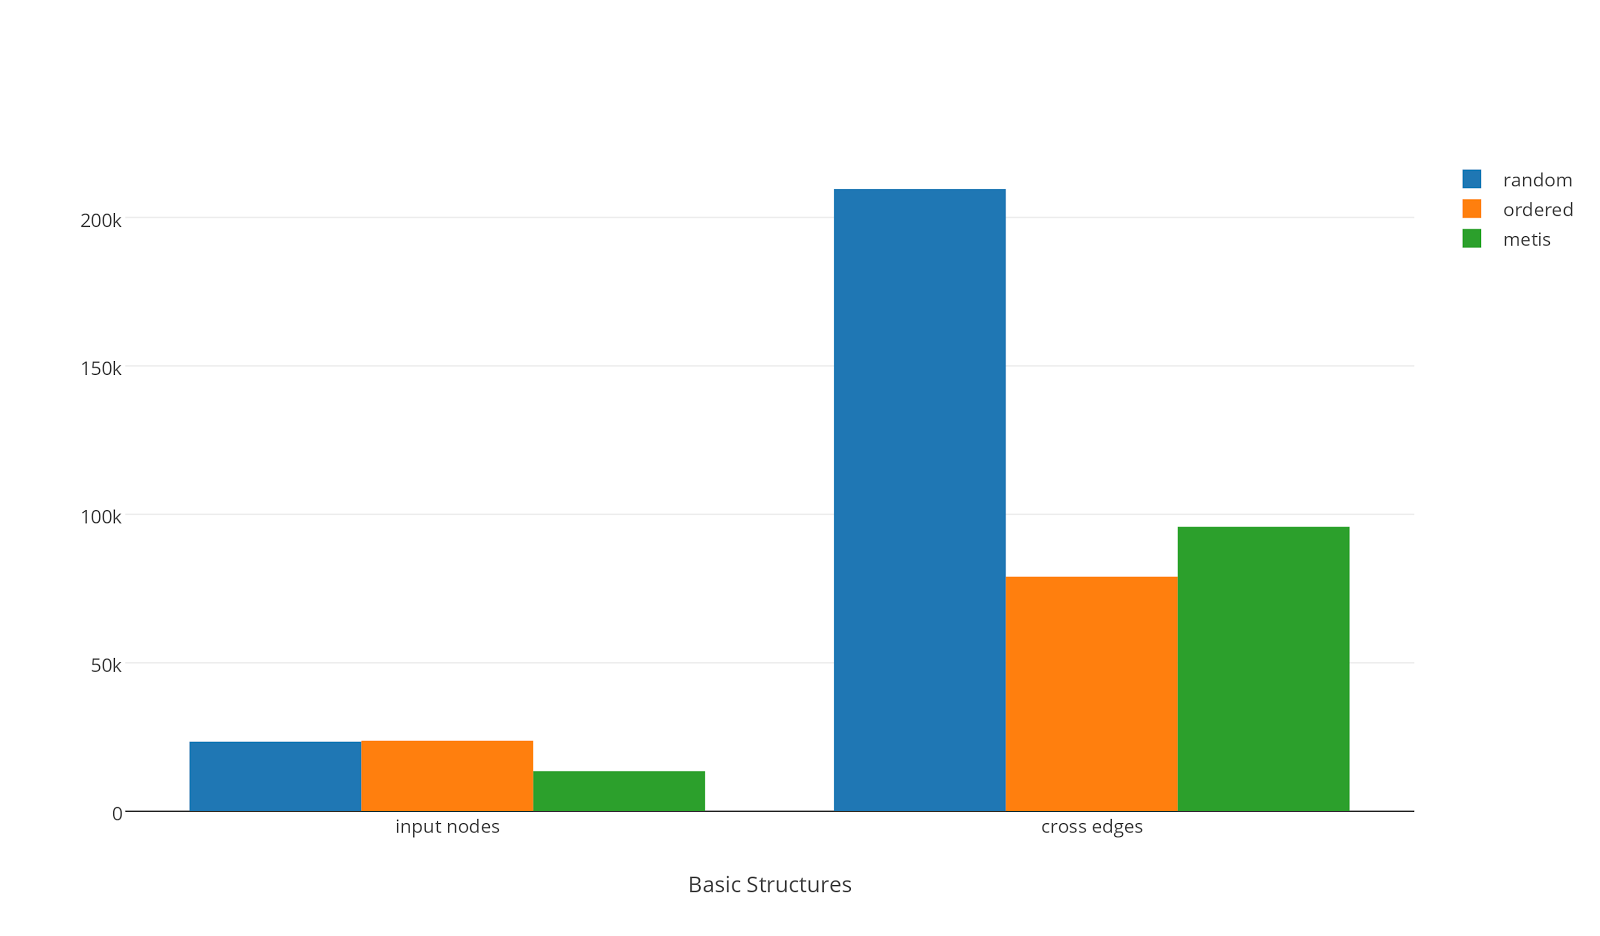
\includegraphics[width=0.8\textwidth]{img/alibaba-structure}
\end{figure}
\\Another interesting finding is that for some queries, different partitioners do not make a difference in the GAG size. In figure \ref{fig:alibaba-Real-World-Queries}, for 8 queries translated from real world, the size of the GAGs are almost the same for different partitioners.
\begin{figure}[h!]
  \caption{GAG Size of Real World Queries}
  \label{fig:alibaba-Real-World-Queries}
  \centering
    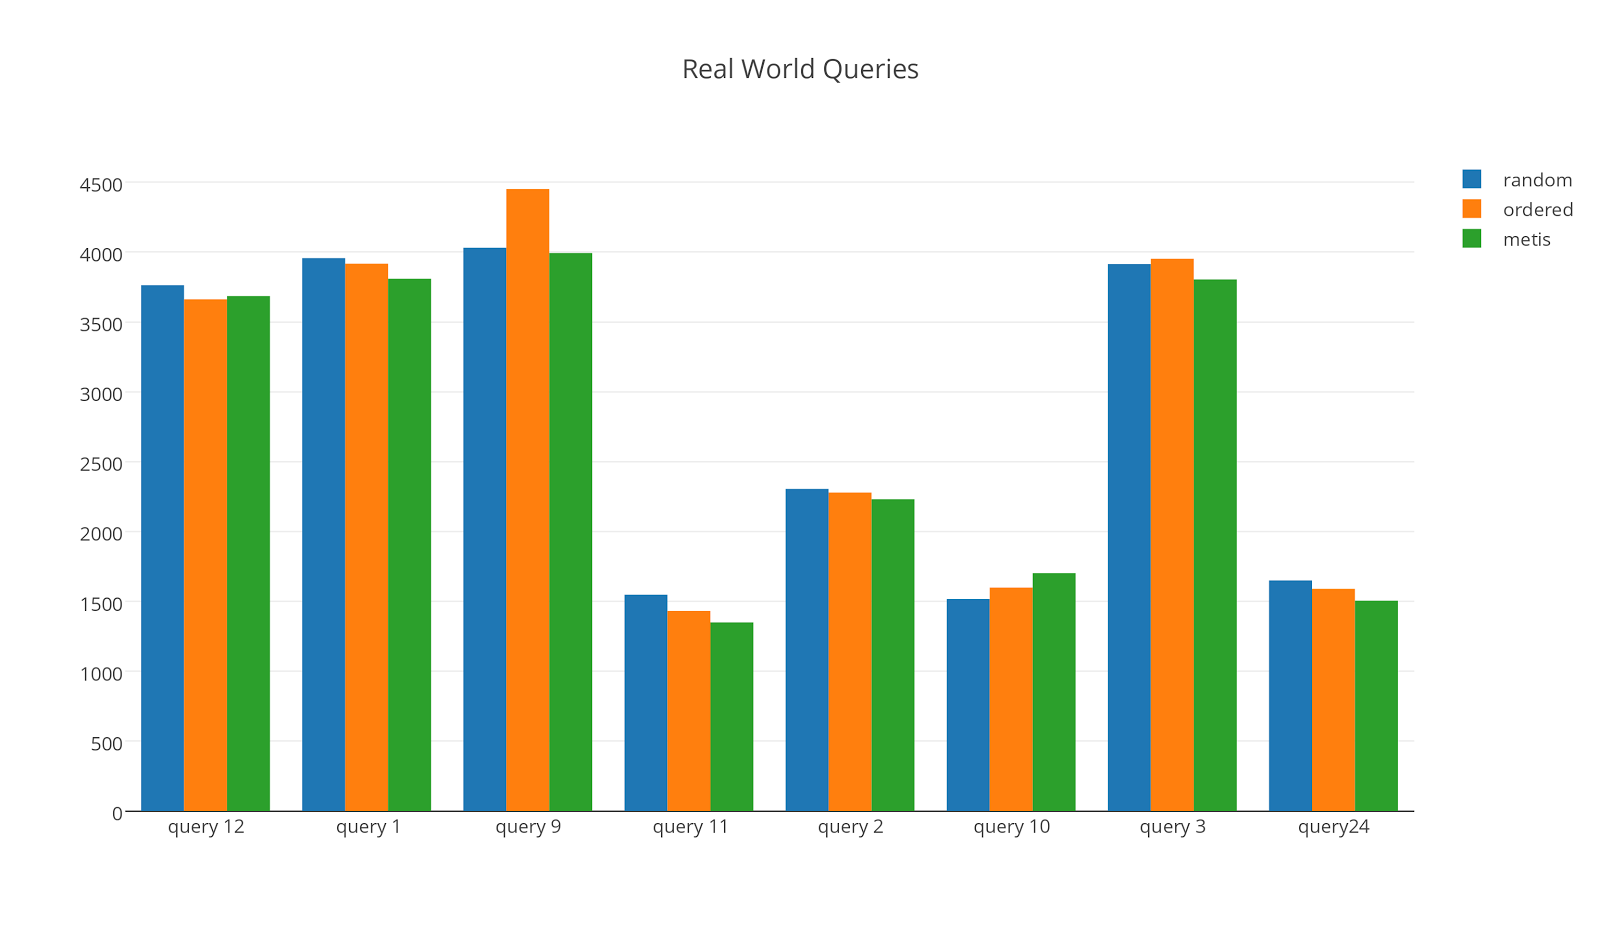
\includegraphics[width=0.8\textwidth]{img/alibaba-Real-World-Queries}
\end{figure}
\\In order to analyze those phenomena, the theoretical size of GAG is analyzed in the next section.
\section{Theoretical Size of GAG}
Recall that the communication cost of the original Dan Suciu's Algorithm is $O(n^2)+O(r)$, where $O(n^2)$ is the size of GAG and $O(r)$ is the size of the result. Actually, the $O(n^2)$ is not always accurate and Dan Suciu gives an  assumption behind it, which we explain in the following.
\\Assuming there are $IN$ input-nodes and $ON$ output-nodes in the distributed graph, then in worst cases, there are $IN*ON*|S|^2$ pairs return to driver side. The assumption behind Dan Suciu's model is that for every input-node there's only one incoming cross-edge, and for each output-node, there's exactly one out cross-edge. Then we can safely conclude that the upper bound of the GAG size is $O(n^2)$.
\\However, in reality not every graph satisfies the model. There can be multiple in-coming cross-edges for one input-node, and multiple out-going cross-edges for one output-node, just like in figure \ref{fig:Cross-Edges}(b), between Dan Suciu's model and fully connected model. Under this model, with a known number of cross-edges, the number of input-nodes can be very different. So we have to focus on algorithms that work with the number of input-nodes now.
\begin{figure}[h!]
  \caption{Different Situations for Cross-Edges}
  \label{fig:Cross-Edges}
  \centering
    \includegraphics[width=0.8\textwidth]{img/Cross-Edges}
\end{figure}
\\So if we extend the case to modified Dan Suciu's Algorithm, the size of GAG, which is also the total communication cost expression, would be:
$$\sum_{\alpha}{(IN_{\alpha}*(|S|-1)+SN_{\alpha})*(ON_{\alpha}*(|S|-1)+FN_{\alpha})}$$
where $IN$ is the number of input-nodes in each site, $|S|$ is the number of states in the automaton, $SN$ is the starting nodes in each site which have out-going edges with same labels as in automata's starting edges, $ON$ is the number of output nodes in each site and $FN$ is the number of nodes where the searching process reaches final states at each site. By the definition of epsilon edges, each output-node in site $\alpha$ has one-on-one relation with one input-node in another site. Then the expression of communication cost would look like:
$$\sum_{\alpha}{(IN_{\alpha}*(|S|-1)+SN_{\alpha})*(\sum_{\beta}{IN_{\beta}}*(|S|-1)+FN_{\alpha})}$$
where $\sum_{\beta}{IN_{\beta}}$ the sum of some input-nodes which connected by epsilon edges from site  $\alpha$.
\\As we start searching from input-nodes and starting-nodes, it's crucial to control their numbers. Generally speaking, for a specific query, $SN$ and $FN$ are fixed, leaving $IN$ the only choice to improve. The expression also explains the phenomenon in figure \ref{fig:alibaba-Real-World-Queries}: For real-world queries whose labels are all rare, $IN*|S|$ is not dominant to $SN$. However, for those queries in figure \ref{fig:alibaba-Random-Queries}, the $SN$ is relatively small, and all labels of non-starting edges in the automaton are quite frequent. Then reducing  $IN$ can improve the performance.
\section{JabeJa Algorithm}
Algorithms 4 and 5 are core parts of the JabeJa Algorithm. At first, each node would be given a color representing its partition. In each round of Algorithm 4, every node $p$ tries to find the best partner which it can swap color with. It communicates with all neighbors first, and if there's no node it can swap color with, it will communicate with a specific random node in the graph. In the end the $p$ exchanges color with its best partner. During the process, simulated-annealing is used to avoid getting stuck in a local optimum and every time a node swaps color successfully, the temperature decreases.
\begin{algorithm}
    \SetKwFunction{proc}{SAMPLEANDSWAP}
    \SetKwProg{myproc}{procedure}{}{endprocedure}
    Require: Any node p in the graph has the following methods:
    \begin{itemize}
        \item $getNeighbors()$: return $p$'s neightbors.
        \item $getRandomSample()$: returns a uniform sample of all the nodes.
        \item $T_0$: the initial temperature.
        \item $\theta$: the cool down speed.
        \item $T_r = T_0$ initially.
    \end{itemize}
    \myproc{\proc{}}{
        \everypar={\nl}
        $partner\leftarrow findPartner(p.getNeighbors(),Tr)$\;
        \If{$partner == null$}{
            $partner \leftarrow findPartner(p.getRandomSample(),Tr)$\;
        }
        \If{$partner \neq null$}{
            handshake for color exchange between $p$ and $partner$\;
        }
        $T_r\leftarrow T_r-\theta$\;
        \If{$T_r<1$}{
            $T_r\leftarrow 1$\;
        }
    }
    \caption{Sample and Swap algorithm at node $p$}
\end{algorithm}
Algorithm 5 describes the way to find the best swap partner. Every time for a node $q$ which $p$ is communicating with, we calculate the degrees of both nodes before and after the swap. If swapping color can decrease the total sum of degrees, it will be compared with the best previous result. In the end, the best partner is returned. The actual swapping operation is implemented as an optimistic transaction, which indicates that the actual swap is done after the two nodes perform a handshake and agree on the swap.
\begin{algorithm}
    \SetKwFunction{proc}{FINDPARTNER}
    \SetKwProg{myproc}{function}{}{endfunction}
    Require: Any node p in the graph has the following methods:
    \begin{itemize}
        \item $getDegree(c)$: return the number of $p$'s neighbors that have color $c$.
    \end{itemize}
    \myproc{\proc{$Node[] \; nodes, float \; T_r$}}{
        \everypar={\nl}
        $highest \leftarrow 0$\;
        $bestPartner \leftarrow null$\;
        \For{$q \in nodes$}{
            $x_{pp} \leftarrow p.getDegree(p.color)$\;
            $x_{qq} \leftarrow q.getDegree(q.color)$\;
            $old \leftarrow x_{pp}+x_{qq}$\;
            
            $x_{pq} \leftarrow p.getDegree(q.color)$\;
            $x_{qp} \leftarrow q.getDegree(p.color)$\;
            $new \leftarrow x_{pq}+x_{qp}$\;
            
            \If{$ (new \times T_r > old) \wedge (new > highest) $ }{
                $bestPartner \leftarrow q$\;
                $highest \leftarrow new$\;
            }
        }
        \Return{$bestPartner$}
    }
    \caption{Find the best node as swap partner for node $p$}
\end{algorithm}
\section{Modified JabeJa Algorithm}
Algorithm 4 remains the same in modified JabeJa algorithm. To minimize the total number of input-nodes in the graph, we  modify the $findPartner$ function, which decreases the number of cross-edges. Algorithm 6 describes the process of finding the best swap partner that reduces the number of input-nodes for a node $p$. The $nodes$ in input parameters is a set of nodes which have different colors from $p$. For every $q$, we call the $CALCDIFF$ function twice to check if swapping color can decrease the number of input-nodes in neighbors of $p$ and $q$. The $CALCDIFF$ function takes two input-nodes $p$ and $q$ and calculates how many nodes in $p$'s neighborhood will turn into input-nodes, and how many input-nodes would turn from input-nodes to an entirely local node. The returning result is a pair $(pinc, pdec)$, which represents the increase and decrease number of input-nodes respectively.
\begin{algorithm}
    \SetKwFunction{proc}{FINDPARTNER}
    \SetKwFunction{calcdiff}{CALCDIFF}
    \SetKwProg{myproc}{function}{}{endfunction}
    \SetKwProg{mycalcdiff}{function}{}{endfunction}
    Require: Any node p in the graph has the following methods:
    \begin{itemize}
        \item $getInDegree()$: return number of $p$'s in-neighbors.
        \item $getInDegree(c)$: return number of $p$'s in-neighbors that have color $c$.
        \item $isInputNode()$: check if $p$ is an input-node.
        \item $getOutNeighbors()$: return $p$'s out-neighbors.
    \end{itemize}
    \myproc{\proc{$Node[] \; nodes, float \; T_r$}}{
        \everypar={\nl}
        $highest \leftarrow 0$\;
        $bestPartner \leftarrow null$\;
        \For{$q \in nodes$}{
            $(pinc,pdec) = CALCDIFF(p,q)$\;
            $(qinc,qdec) = CALCDIFF(q,p)$\;
            $old \leftarrow pinc+qinc$\;
            $new \leftarrow pdec+qdec$\;
            \If{$ (new \times T_r > old) \wedge (new > highest) $ }{
                $bestPartner \leftarrow q$\;
                $highest \leftarrow new$\;
            }
        }
        \Return{$bestPartner$}
    }
    \mycalcdiff{\calcdiff{$Node \; p, Node \; q$}}{
        \everypar={\nl}
        $pNeighbors \leftarrow p.getOutNeighbors()\backslash q.getOutNeighbors()\backslash \{q\}$\;
        $pinc \leftarrow 0$\;
        $pdec \leftarrow 0$\;
        \For{$k \in pNeighbors$}{
            \If{$k.isInputNode() = false$}{
                $pinc \leftarrow pinc + 1$\;
            }
            \If{$k.getInDegree(k.color) = k.getInDegree()-1 \wedge q.color = k.color$}{
                $pdec \leftarrow pdec + 1$\;
            }
        }
        \If{$p \notin q.getOutNeighbors() \wedge p.getInDegrees()>0$ }{
            \If{$p.isInputNode() = false$}{
                $pinc \leftarrow pinc + 1$\;
            }
            \ElseIf{$p.getInDegree(q.color) = p.getInDegree()$}{
                $pdec \leftarrow pdec + 1$
            }
        }
        \Return{$(pinc,pdec)$}
    }
    \caption{Find the best swap partner that minimize \#$inputnodes$ for node $p$}
\end{algorithm}
\\The body of function $CALCDIFF$ can be explained with the help of figure \ref{fig:modified-dan-example}, here we call nodes that are not input-nodes local-nodes.
\\Line 15-16 initialize the increase and decrease number of input-nodes to be 0.
\\Line 14 ensures that nodes which are out-neighbors of both $p$ and $q$, get ignored since swapping color would not change the node status (Figure \ref{fig:modified-dan-example}(a)). At the same time, $q$ is a special case and needs to be considered separately. 
\\Line 17-24 explains the process of examining the status of each node in $pNeighbors$: 
\begin{enumerate}
    \item If it's currently not a input-node, then after swapping it would definitely be a input-node since new color of $p$ is different (Figure \ref{fig:modified-dan-example}(b)).
    \item If it's currently a input-node, has same color with $q$ and $p$ is the only node with different color, then current node will turn from input-node to a local-node (Figure \ref{fig:modified-dan-example}(c)).
\end{enumerate} 
Line 25-31 explains the process of examining the status of $p$:
\begin{enumerate}
    \item If $p$ is one of $q$'s neighbors or its in-degree is 0, swapping color would makes no difference for $p$'s status.
    \item If $p$ is not a input-nodes, swapping color would make it becomes a input-node (Figure \ref{fig:modified-dan-example}(d)).
    \item If all of $p$'s has same number of in-neighbors of $q$'s color as in-degree, swapping color turns $p$ from input-node to a local-node (Figure \ref{fig:modified-dan-example}(e)).
\end{enumerate}
\begin{figure}[h!]
  \caption{Different Situations for Examining Input-Nodes}
  \label{fig:modified-dan-example}
  \centering
    \includegraphics[width=1.0\textwidth]{img/modified-dan-example}
\end{figure}
In theory, the more nodes $p$ tries to swap with in every iteration, the larger the chance is that it goes to the best result. If every time $p$ communicates with all other nodes in graph, it would choose the best swap partner in theory, even if it's very time-consuming. So in polynomial time  $O(|V|^2)$ a given partitioning situatjion can be checked if it's the best solution, if we assume the $FINDPARTNER$ function takes one unit time.
\section{Evaluation}
Every node in the graph runs Algorithm 4 concurrently. Similar to the Original JabeJa algorithm, the actual swap is done after the two nodes perform a handshake and agree on the swap. As function $getInDegree(c)$ would access shared data which could be updated after a swap, the algorithm should be implemented with an asynchronous programming model. Under this circumstance, Spark is not suitable for implementation. Although there is a simple implementation\cite{jabejagraphchi} of JabeJa algorithm on GraphChi\cite{kyrola2012graphchi}, a disk-based graph computing system based on the asynchronous model, it's still time-consuming to study a new platform and code in a new programming model. We focus on comparing the number of input-nodes, but not the offline performance of the algorithms. So we implemented the modified JabeJa Algorithm sequentially and simulated the result.
\subsection{Approach}
The experiment steps are as followed:
\begin{enumerate}
    \item Generate random graphs and queries with GMark Benchmark. The graphs have $10^5$, $10^6$, and $10^7$ nodes respectively. We stop at $10^7$ as the size of $GAG$ has upper bound $(|V||S|)^2$ and it might be very expensive to compute on the driver for a larger graph.
    \item Check the queries, keep those which start with rare labels and delete those which take longer than 1 hours to solve sequentially.
    \item Run four partition strategies against those graphs with different partition numbers and check the number of input-nodes in each setting. For the METIS algorithm, we use the available library at \cite{metislib}. For JabeJa and modified JabeJa, we use the single-thread program mentioned above.
    \item Use the modified Dan Suciu's algorithm to evaluate random queries in step 2 on top of graphs with different partition strategies, and compare the size of GAG, running time and driver-side computation time for each query.
\end{enumerate}
\subsubsection{Parameter Selection} We set initial temperature $T_0 = 2$ and cool down speed $\theta = 0.01$ in simulated annealing, which is similar to existing implementation in GraphChi. Each iteration the program calls $FINDPARTNER$ for every node. If there are no neighbors to swap with, we choose five random nodes with different colors for it and call $FINDPARTNER$ again. The program terminates when the input-nodes number remains the same for ten iterations.
\subsection{Metrics}
We observed the following:
\begin{enumerate}
    \item Input-Nodes: The main property to investigate. We will try to find out the relation between input-nodes number and running time of the algorithm.
    \item Cross-Edges: When two partition strategies have a close number of input-nodes, the one with fewer cross-edges is preferred as it might be optimal for other kinds of query algorithms in a graph database.
    \item Size of the GAG: The amount of data transmitted in the network. It could also affect the performance on the driver side.
    \item Driver-Computation Time: The computation time after the driver receives GAG. This is investigated for the queries whose evaluation bottleneck is on the driver side.
    \item Overall Running Time: The total time spent on solving each query.
\end{enumerate}

\subsection{Research Questions}
The research questions related to the metrics can be formulated as followed:
\begin{enumerate}
    \item How does JabeJa* perform in minimizing input-node number comparing to other partitioners?
    \item As the input-node number decreases, will the size of GAG decreases?
    \item As the GAG size decreases, will the driver computation time decreases?
    \item As the GAG size decreases, will the overall evaluation time decreases?
\end{enumerate}

\subsection{Input-Nodes and Cross-Edges}
In this part, the number of input-nodes and cross-edges are listed along with the different number of partitions. For the legends, the suffix `ce' is short for cross-edge and `in' is short for input-node. `JabeJa*' represents the modified JabeJa Algorithm. Sometimes the default partitioner is also written as 'ordered' as it's the basic approach of the partitioner.
\subsubsection{Alibaba}
For Benchmark Alibaba, the number of cross-edges and input-nodes are shown in Figure \ref{fig:Alibaba-Partitioners}: Both of the numbers become relatively stable when we divide the graph into 32 partitions. The interesting findings are:
\begin{enumerate}
    \item METIS turns out to be optimal in reducing input-nodes. However, it does not lead to the best number of cross-edges, which the algorithm is developed to optimize initially.
    \item JABEJA beats METIS in the number of cross-edges, but the input-nodes number is still around $50\%$, which is far from the best.
    \item The modified JabeJa Algorithm cuts the number of input-nodes compared to original JabeJa algorithm, but as a trade-off, the number of cross-edges is much worse than with the JabeJa algorithm.
    \item Most of the time, the random and default partitioner are worst in both the number of cross-edges and the number of input-nodes. However, the default partitioner has a good number of cross-edges when there are only a few partitions.
\end{enumerate}
\begin{figure}[h!]
  \caption{Input-node and Cross-edge size of Alibaba Graph}
  \label{fig:Alibaba-Partitioners}
  \centering
    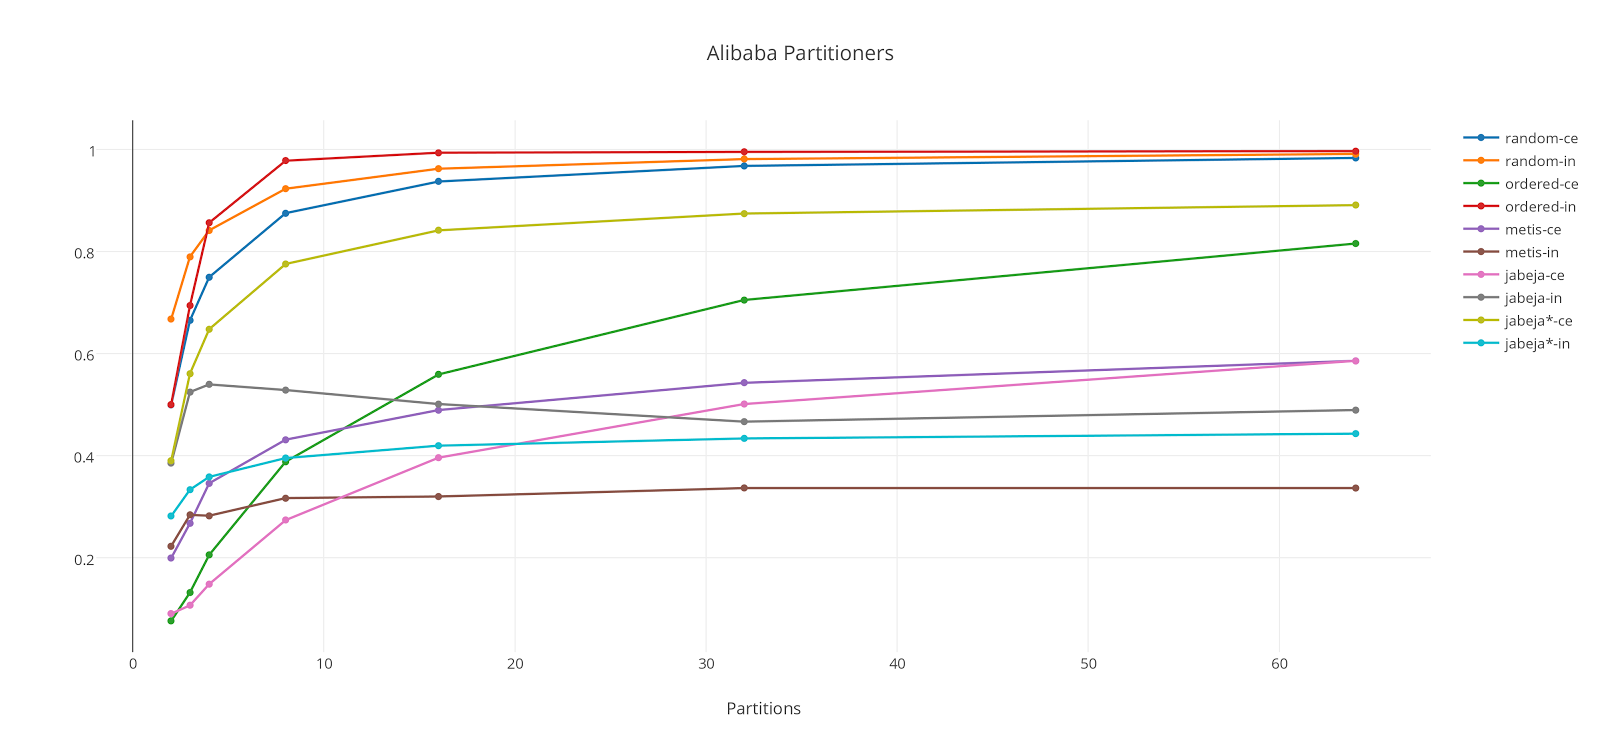
\includegraphics[width=1.0\textwidth]{img/Alibaba-Partitioners}
\end{figure}

\subsubsection{YouTube}
For the YouTube Benchmark, the ratio of cross-edges and input-nodes compared to corresponding total numbers are presented in Figure \ref{fig:Youtube-Partitioners}. The main observations are:
\begin{enumerate}
    \item JabeJa has the least cross-edges and even beats METIS.
    \item JabeJa* has the largest number of cross-edges, which is worse than default-partitioners.
    \item The number of input-nodes for non-default partition strategies are all close to 100\% and don't vary with the increase number of partitions. In this case, default partitioning strategy outperforms the strategies we discussed, which suggests that for a dense graph, those algorithm can barely improve the number of input-nodes.
\end{enumerate}
\begin{figure}[h!]
  \caption{Input-node and Cross-edge size of YouTube Graph}
  \label{fig:Youtube-Partitioners}
  \centering
    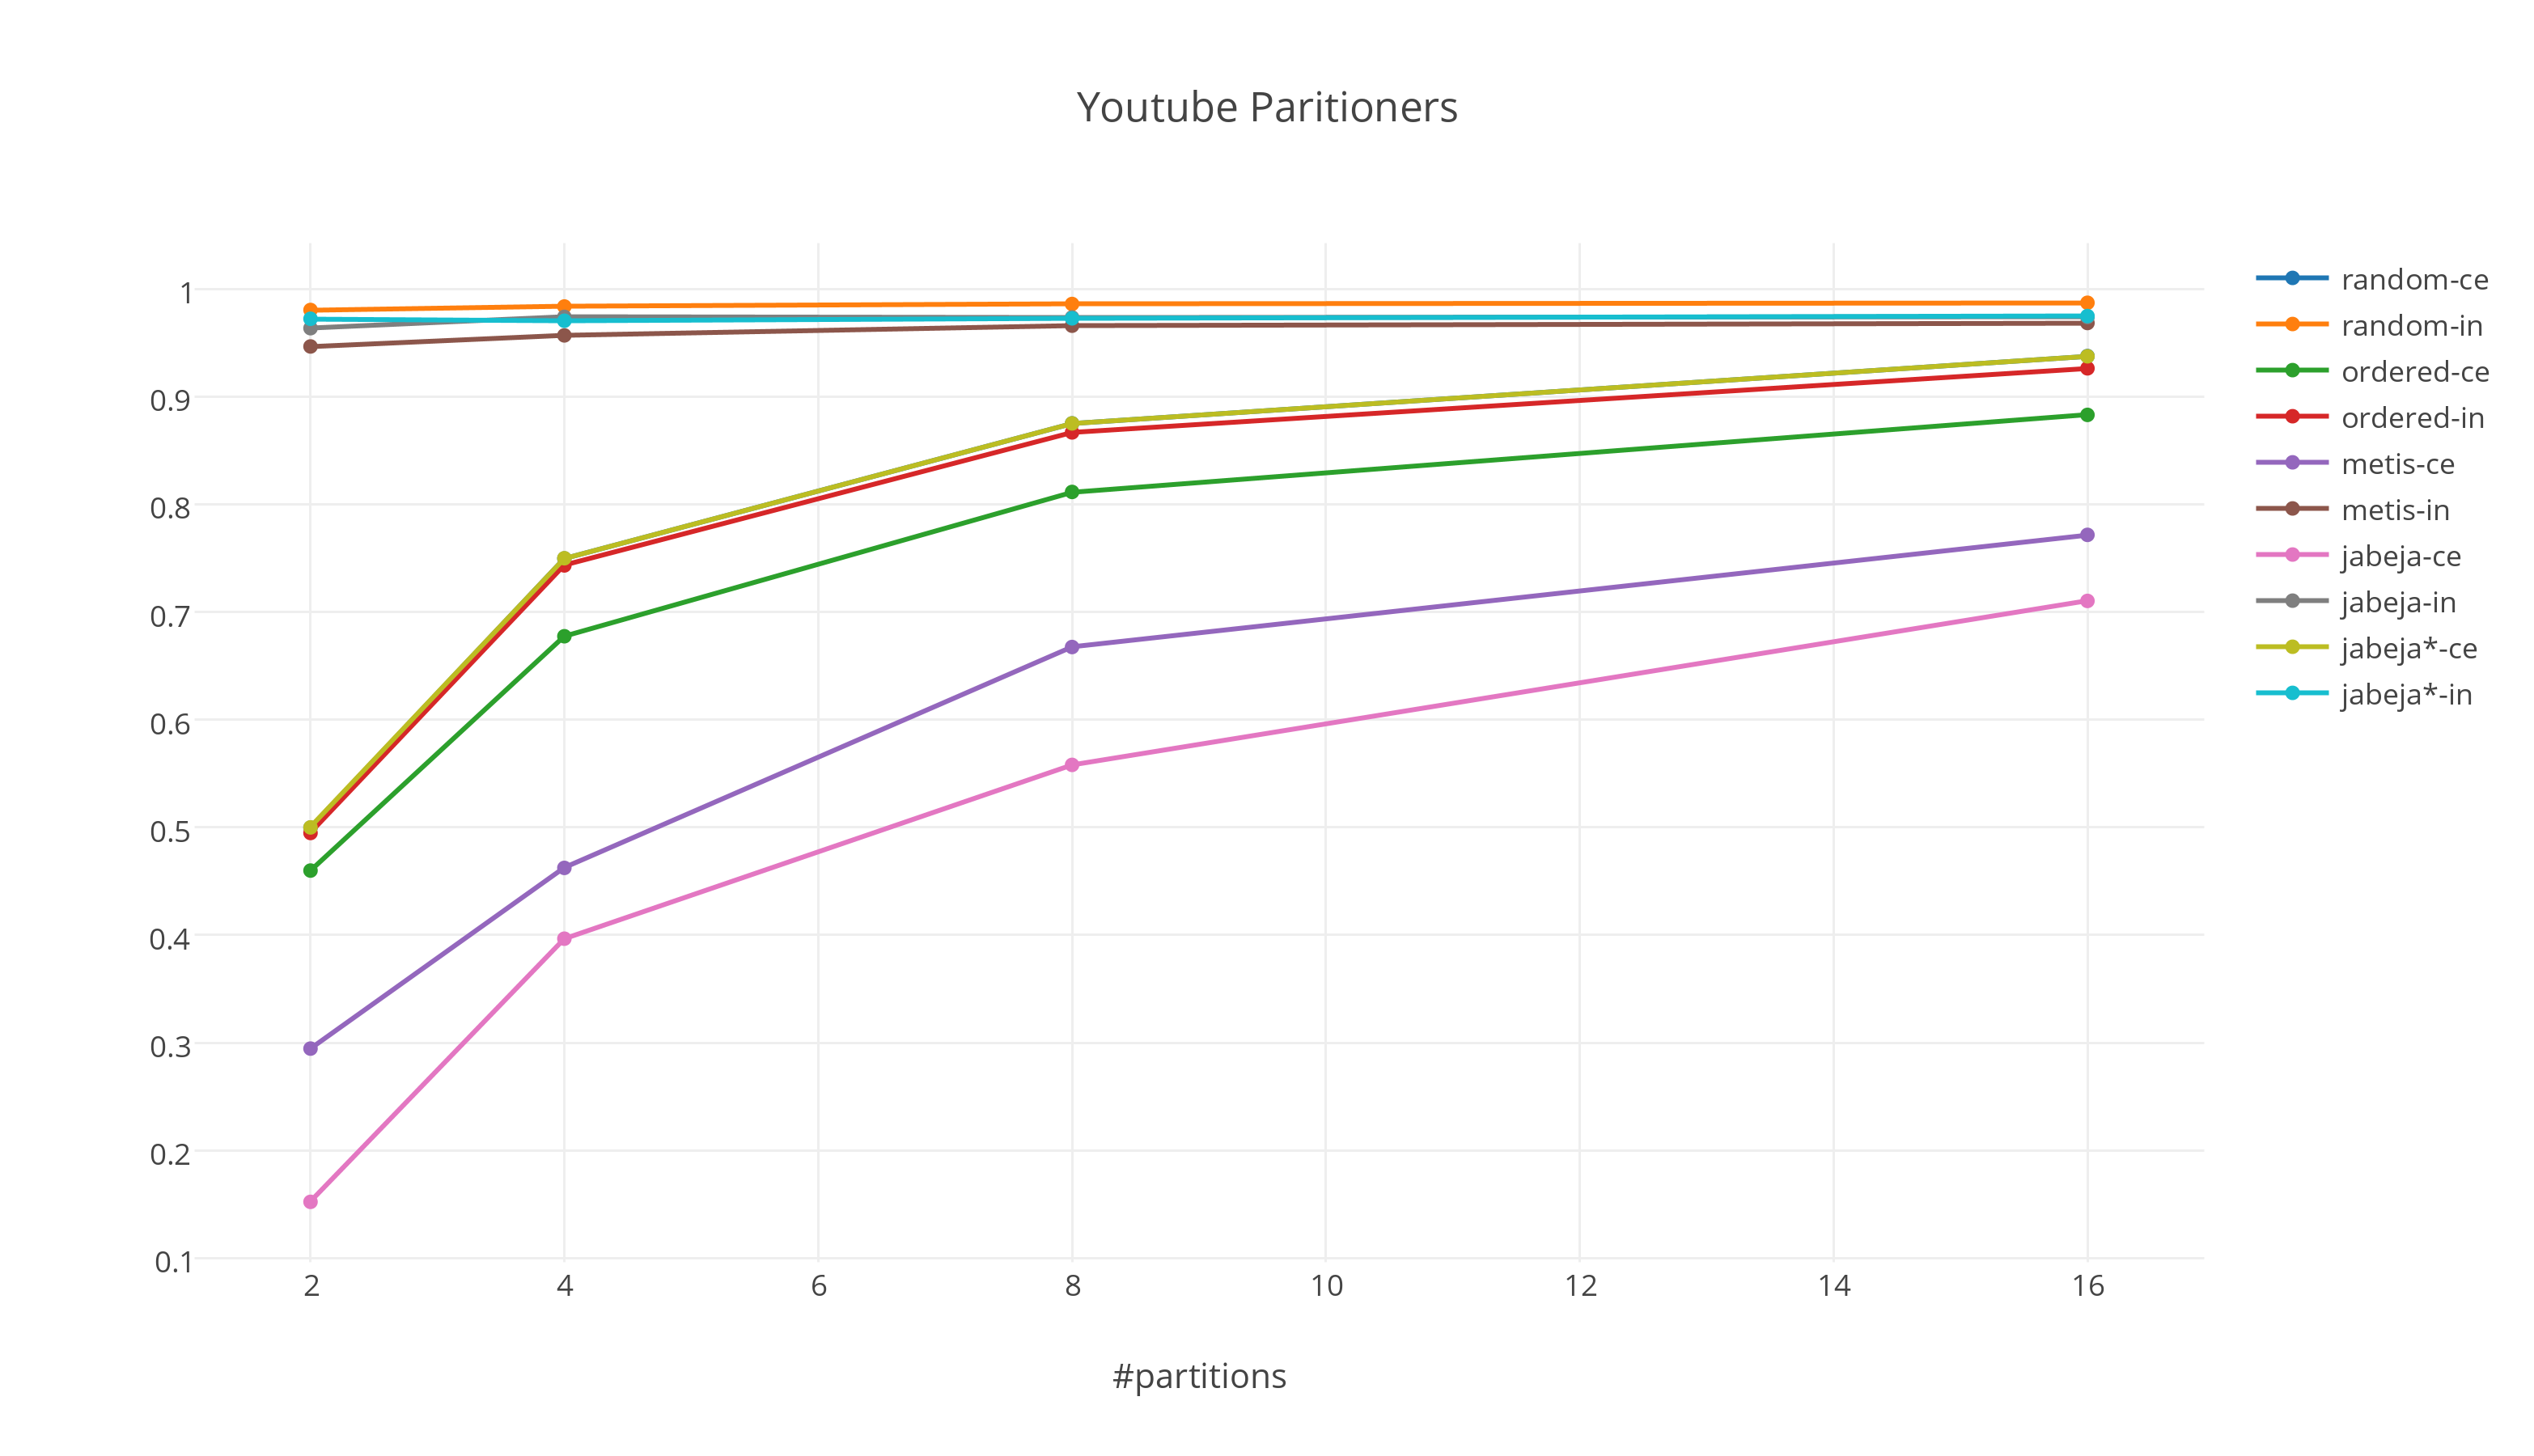
\includegraphics[width=1.0\textwidth]{img/Youtube-Partitioners}
\end{figure}

\subsubsection{Higgs}
For Benchmark Higgs, Figure \ref{fig:Higgs-Partitioners} shows the ratio of cross-edges and input-nodes. The followings are key findings:
\begin{enumerate}
    \item The METIS strategy has the least input-nodes with various numbers of partitions.
    \item JabeJa is slightly better than METIS with regards to cross-edges in the end, and is the best when there are 16 partitions.
    \item JabeJa* is not improving both the numbers of input-nodes and cross-edges.
\end{enumerate}
\begin{figure}[h!]
  \caption{Input-node and Cross-edge size of Higgs Graph}
  \label{fig:Higgs-Partitioners}
  \centering
    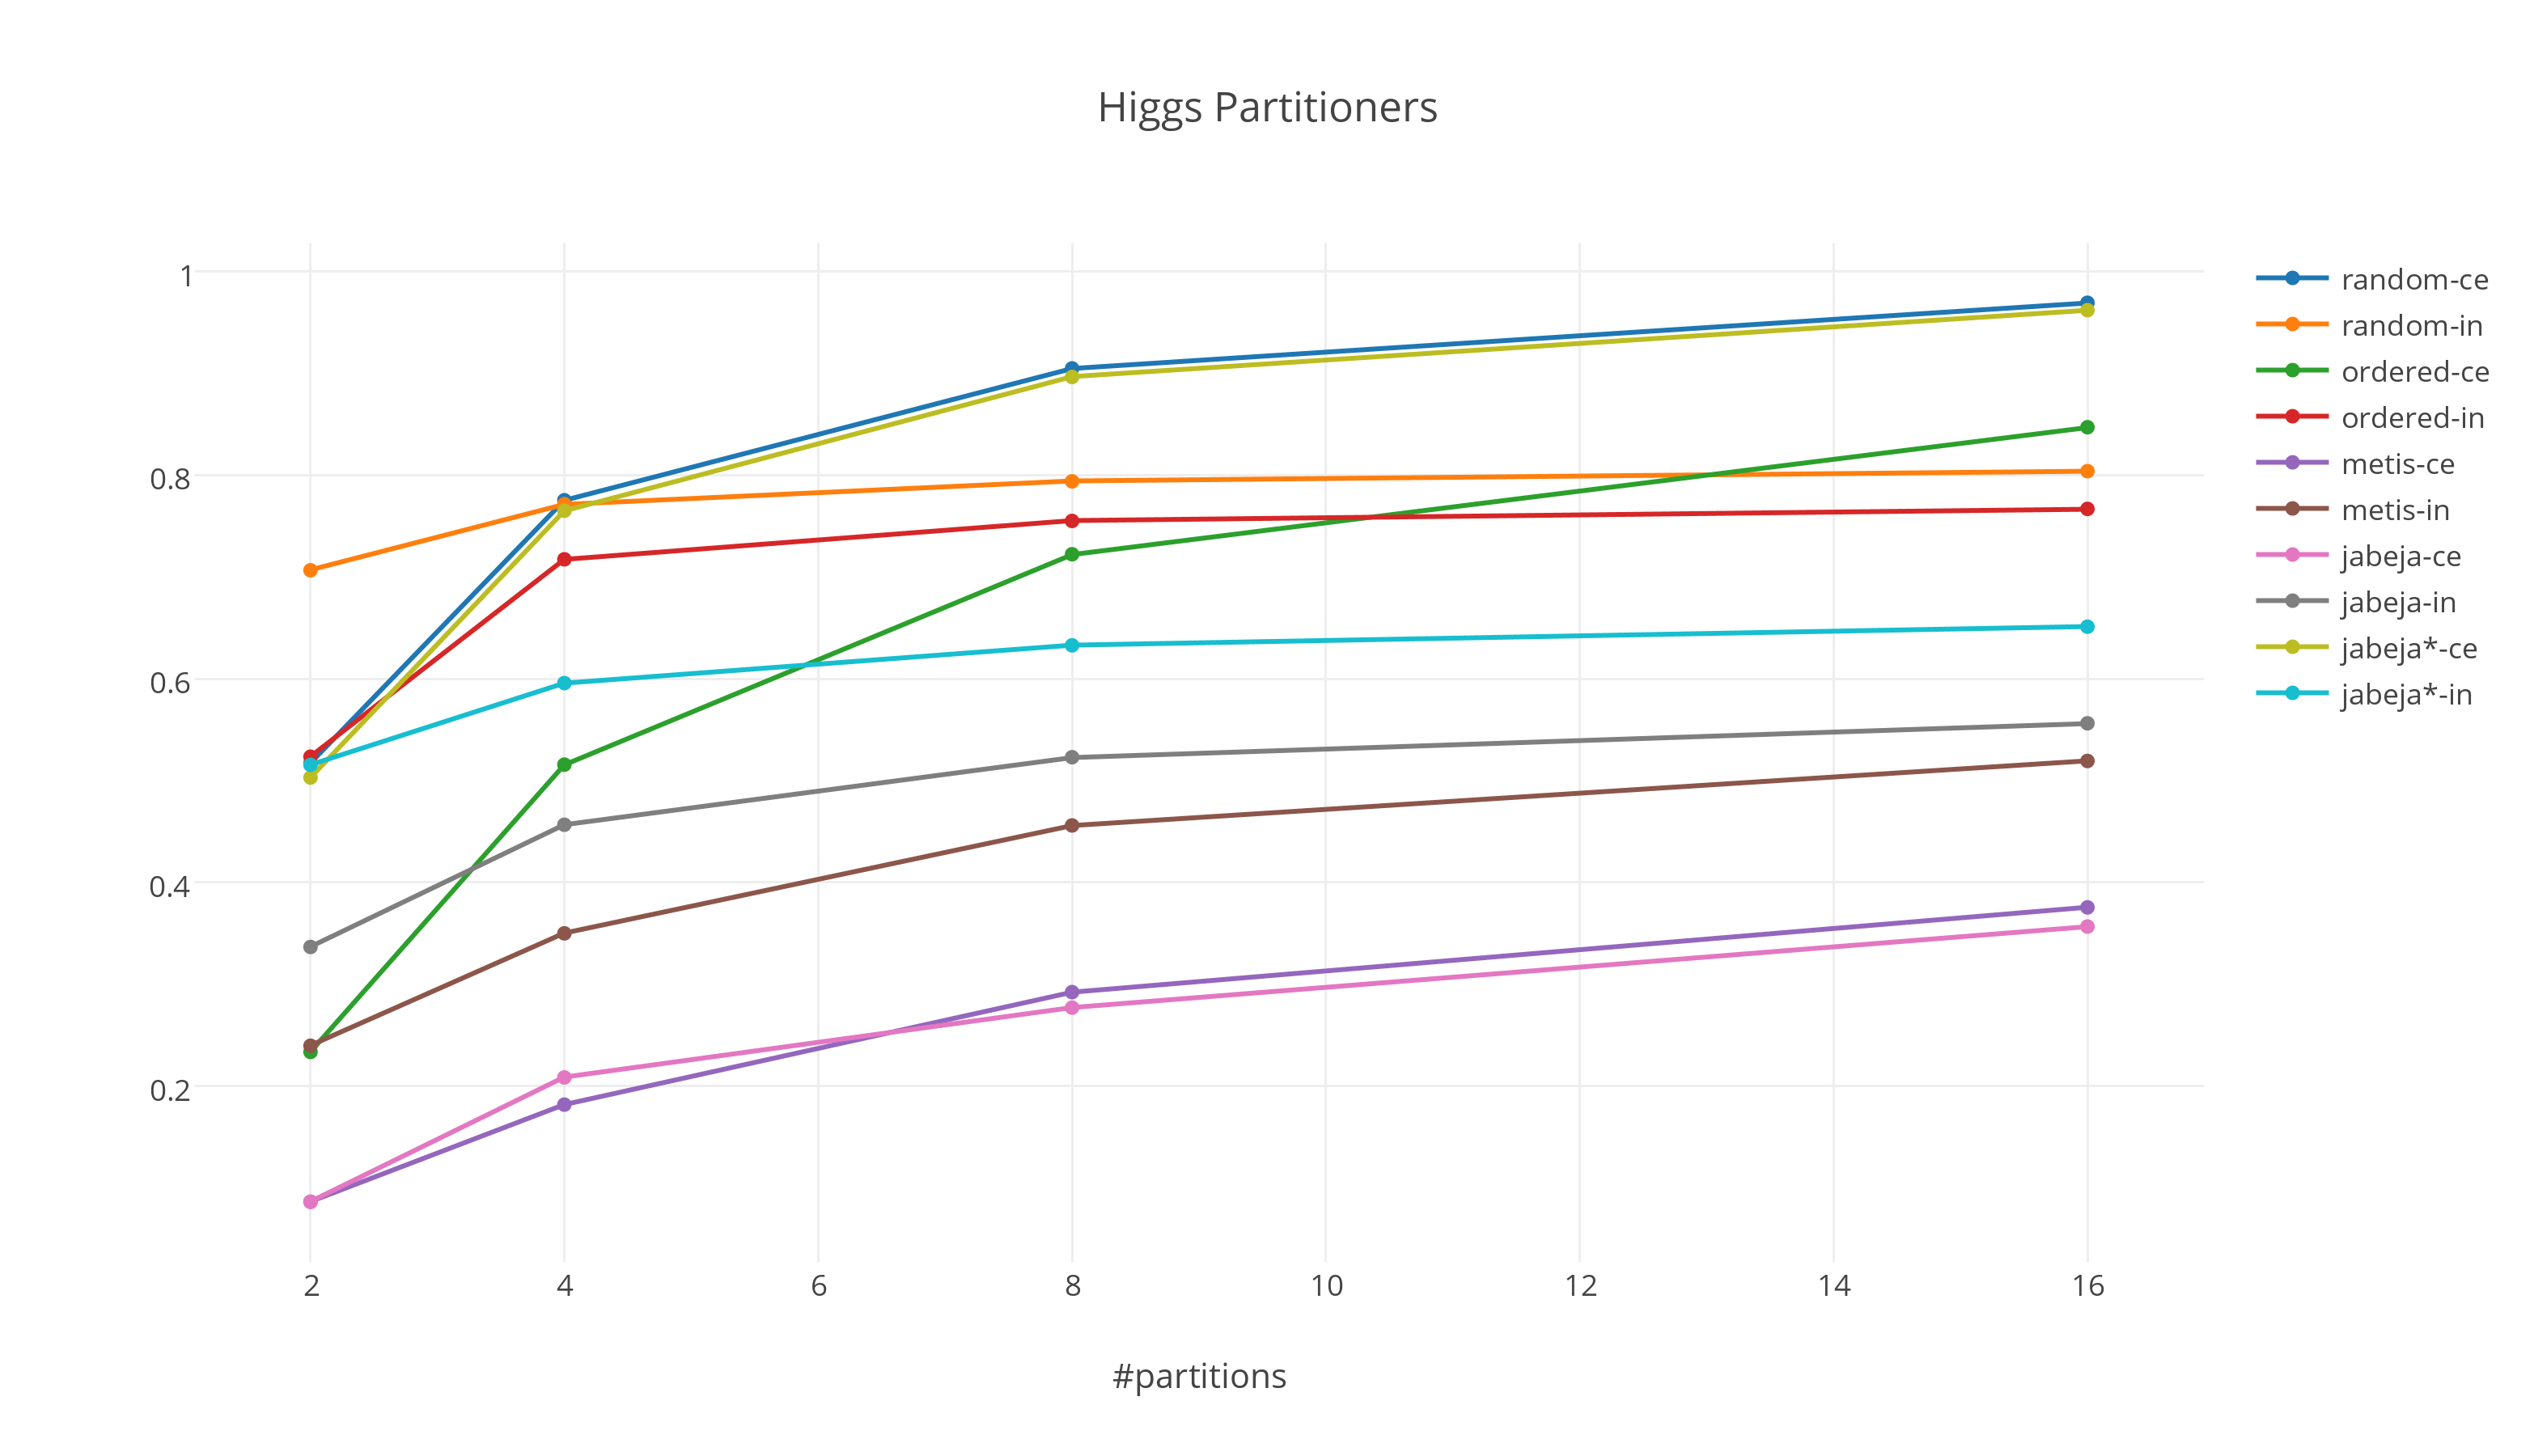
\includegraphics[width=1.0\textwidth]{img/Higgs-Partitioners}
\end{figure}


\subsubsection{GMark Graphs}
We run those partition strategies against three GMark Graphs. The result is as in Figure \ref{fig:0.1m-inputnode}, Figure \ref{fig:1m-inputnode} and Figure \ref{fig:10m-inputnode}. We can see that the three diagrams are almost the same in shape, except the values are multiplied by ten. The number of input-nodes and cross-edges are relatively stable at eight partitions. The interesting findings are:
\begin{enumerate}
    \item This time METIS beats all partition strategies in both input-node and cross-edge number. The number of input-nodes is below $10\%$ of $|V|$, which is an excellent result.
    \item The modified JabeJa Algorithm is slightly better than JabeJa Algorithm concerning with input-node number, but finally they are almost the same when the graph is in 16 partitions.
    \item The default partitioner is worst all the time in input-node and cross-edge numbers. The reason behind it might be that the GMark graphs are randomly generated, unlike Alibaba as a real-world and well-organized benchmark.
\end{enumerate}
\begin{figure}[h!]
  \caption{Input-node and Cross-edge size of GMark Graph ($10^5$ nodes)}
  \label{fig:0.1m-inputnode}
  \centering
    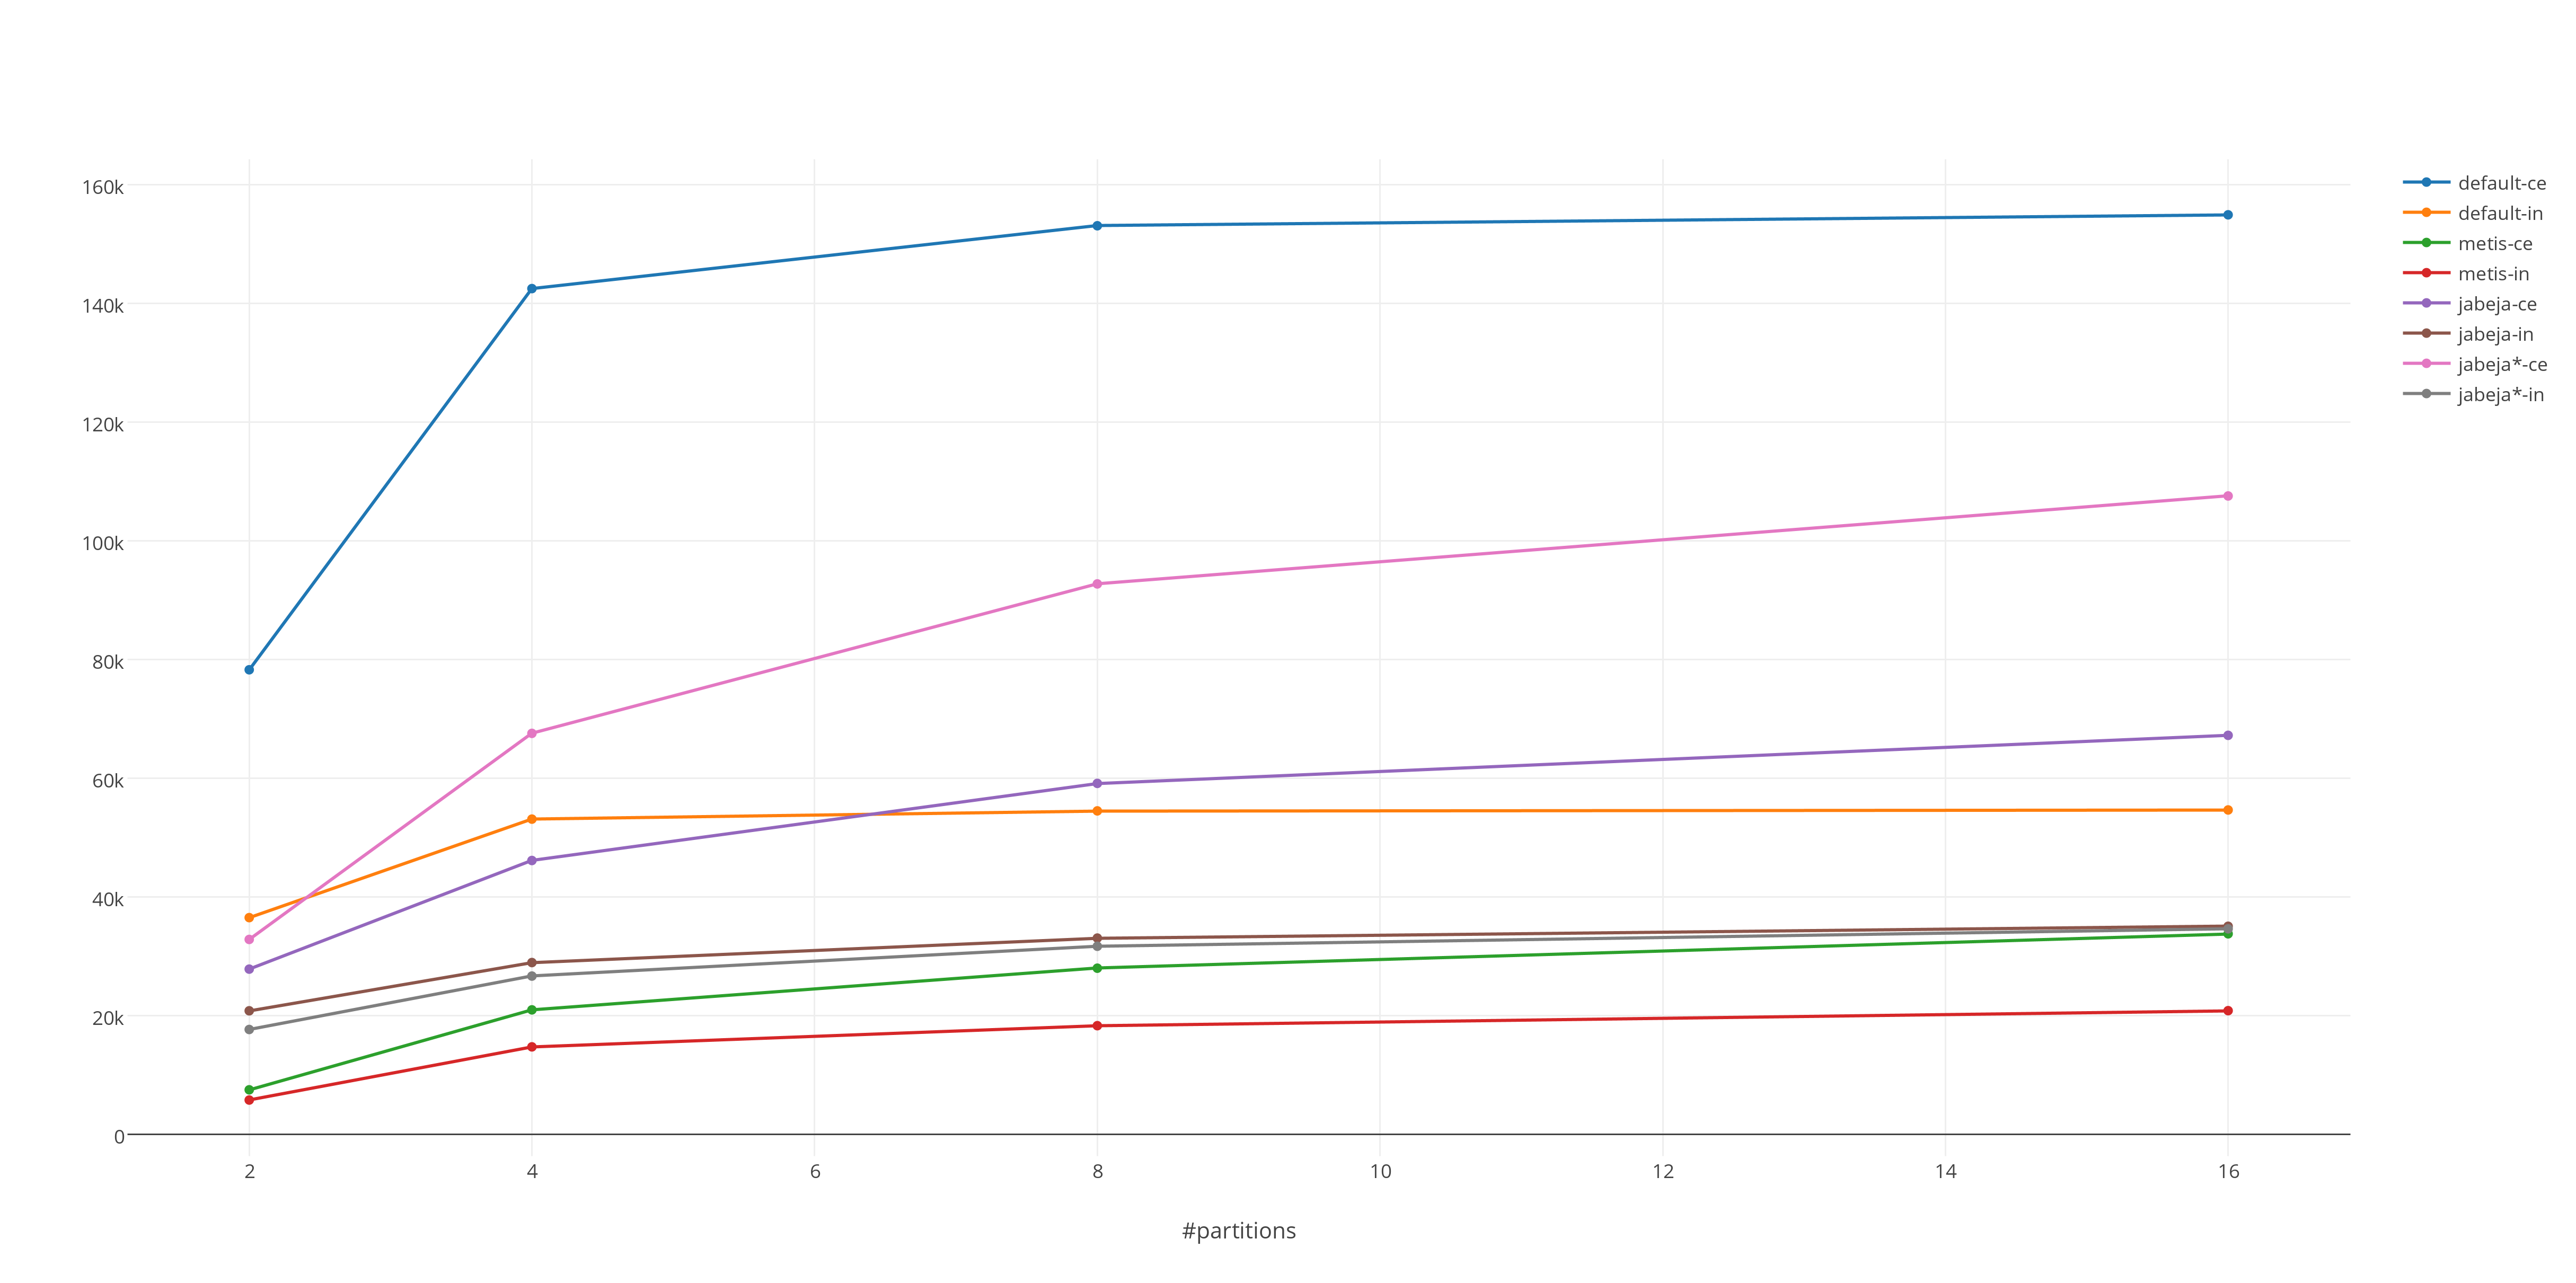
\includegraphics[width=1.0\textwidth]{img/-1m-inputnode}
\end{figure}
\begin{figure}[h!]
  \caption{Input-node and Cross-edge size of GMark Graph ($10^6$ nodes)}
  \label{fig:1m-inputnode}
  \centering
    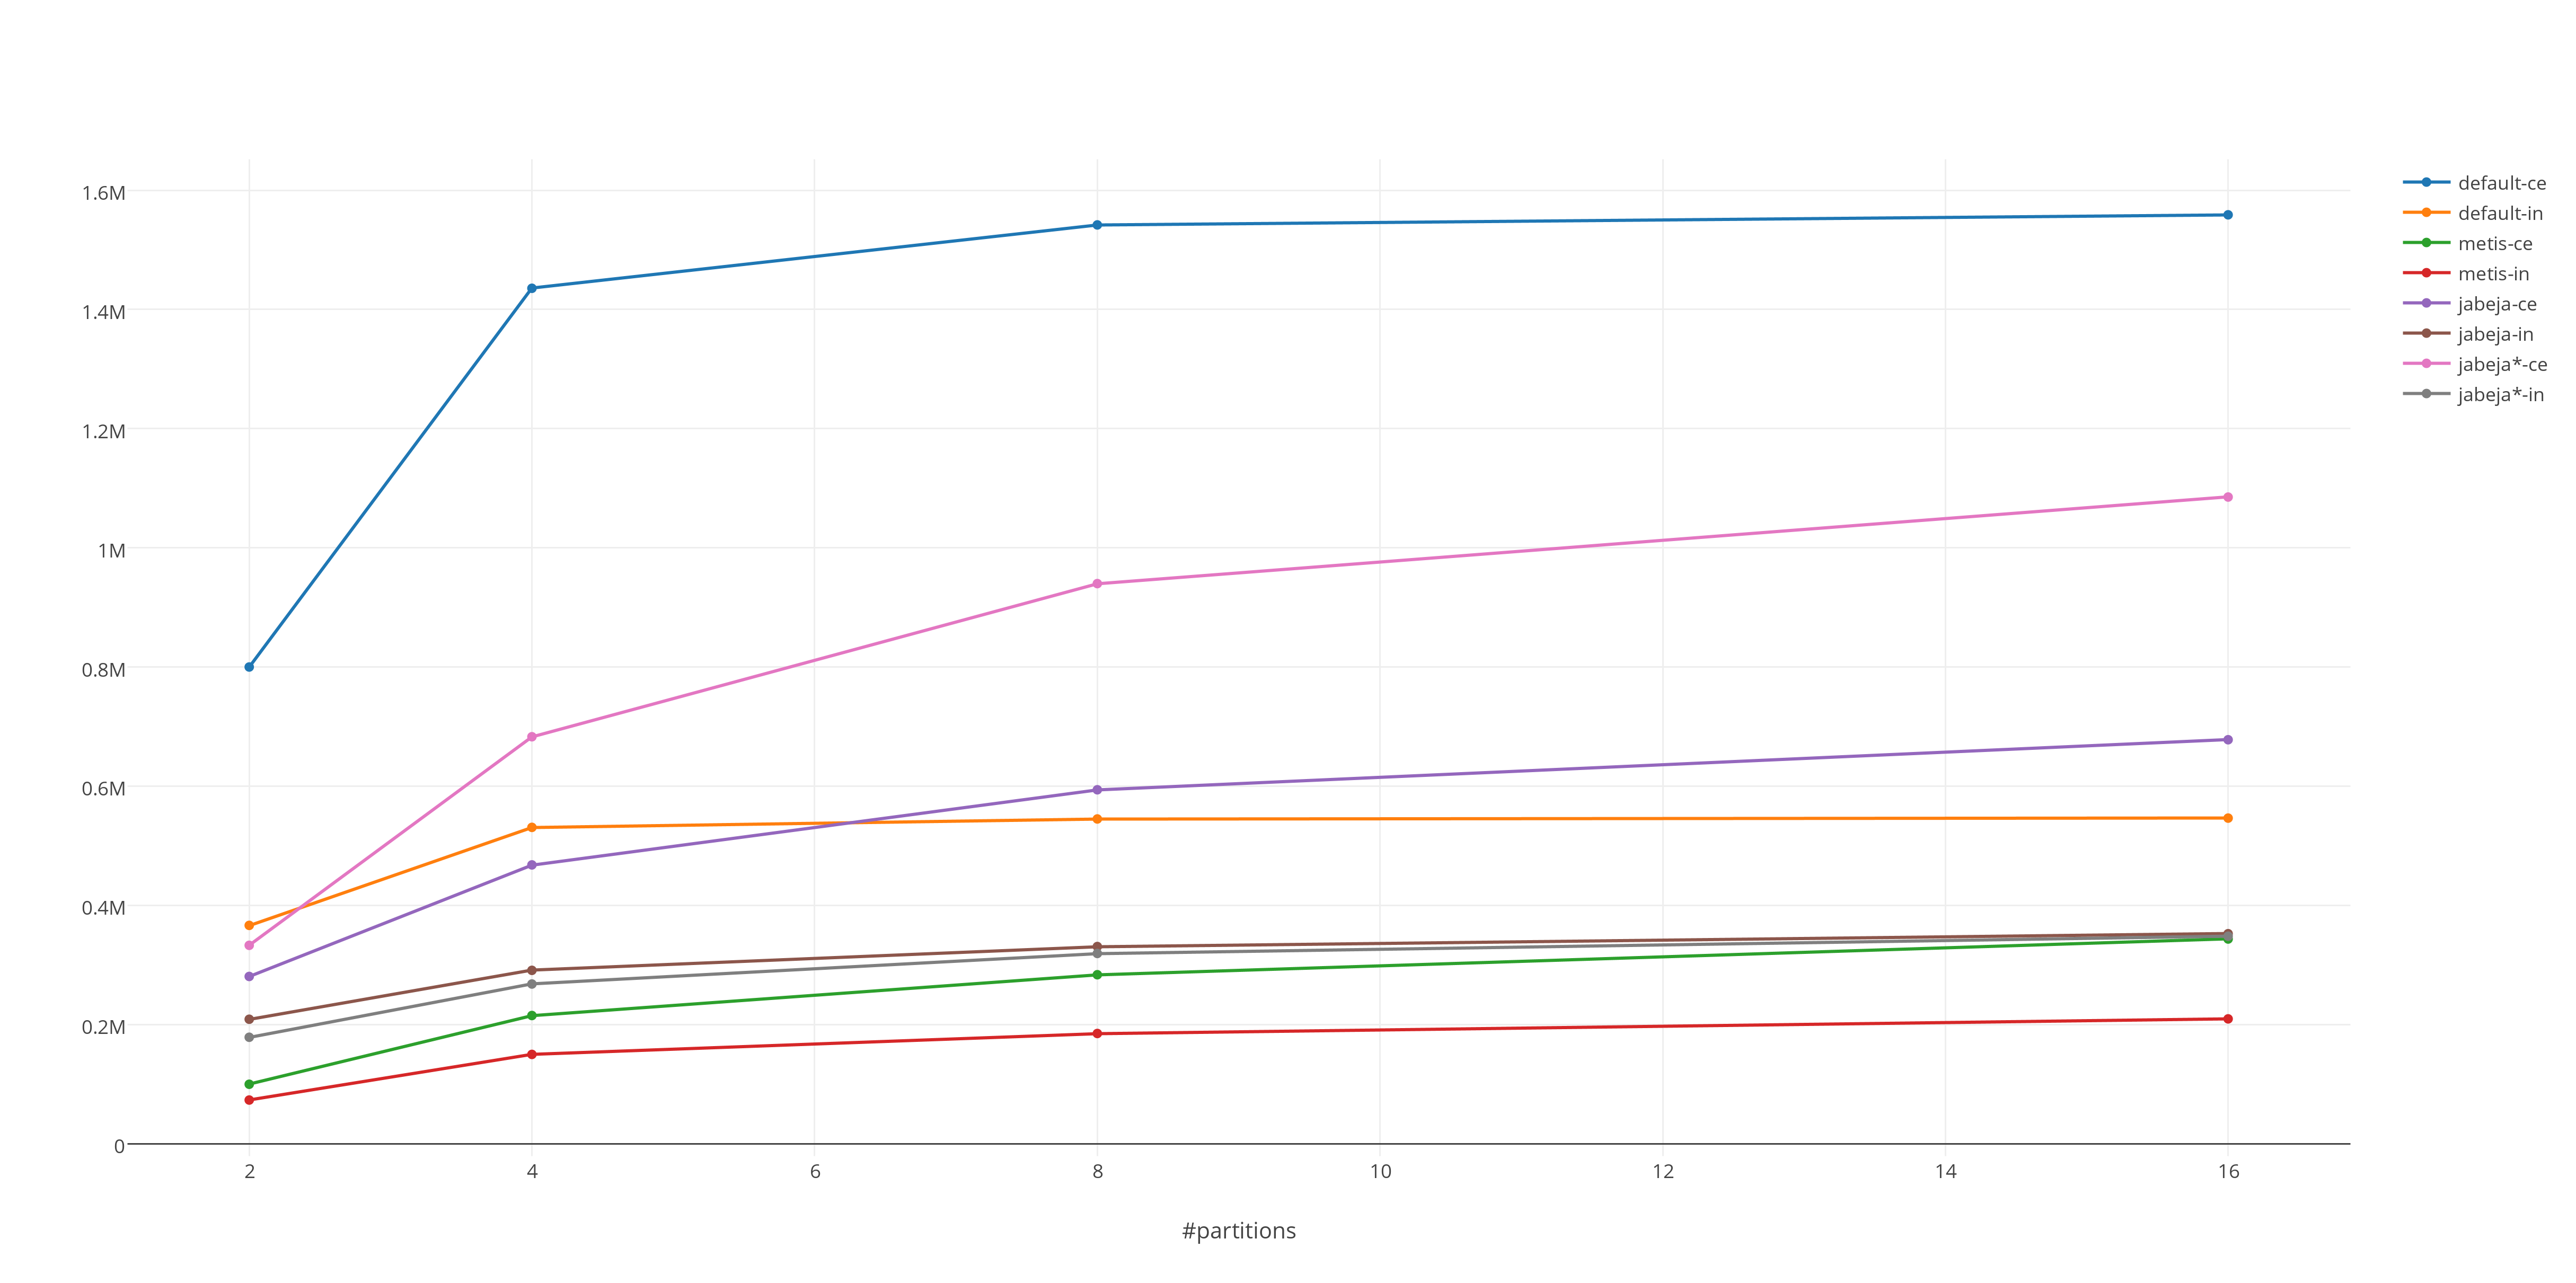
\includegraphics[width=1.0\textwidth]{img/1m-inputnode}
\end{figure}
\begin{figure}[h!]
  \caption{Input-node and Cross-edge size of GMark Graph ($10^7$ nodes)}
  \label{fig:10m-inputnode}
  \centering
    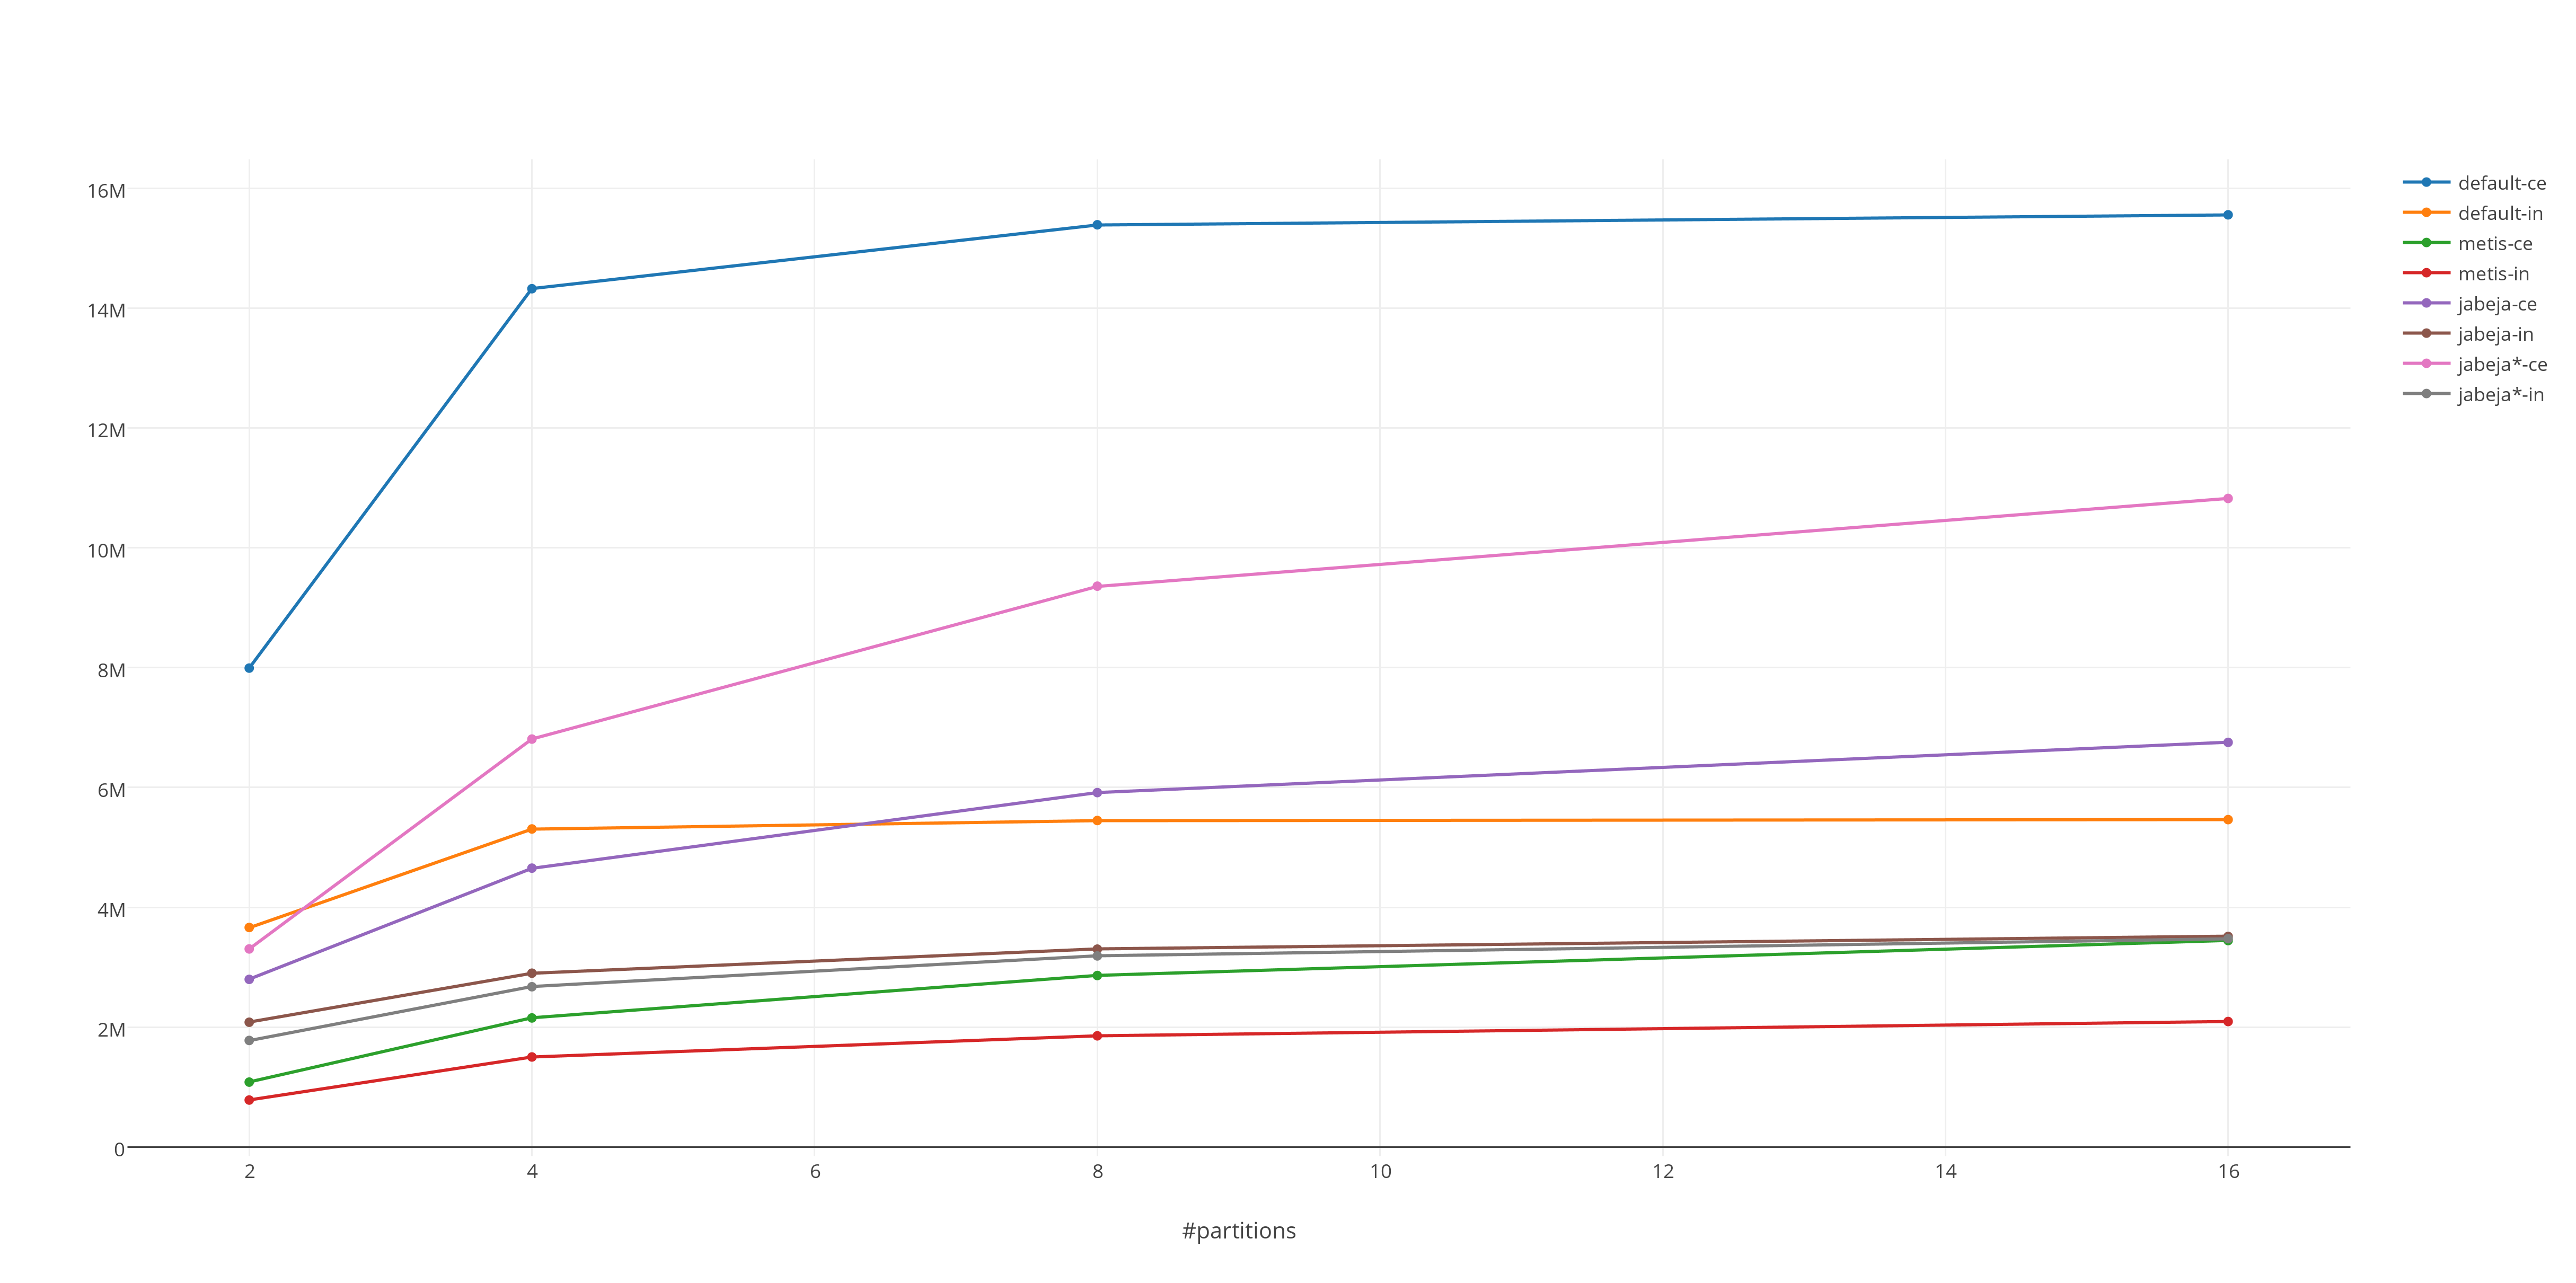
\includegraphics[width=1.0\textwidth]{img/10m-inputnode}
\end{figure}

\subsection{Size of the GAG}
As the number of input-nodes is relatively stable with eight partitions, we run Dan Suciu's Algorithm on GMark graphs split by different strategies with eight workers. The size of GAG can be found in Figure \ref{fig:gmark-01m-gag}, Figure \ref{fig:gmark-1m-gag} and Figure \ref{fig:gmark-10m-gag}. For each query, we list the number of pairs in GAG with different partition strategies.
\begin{figure}[h!]
  \caption{GAG size of GMark Graph ($10^5$ nodes)}
  \label{fig:gmark-01m-gag}
  \centering
    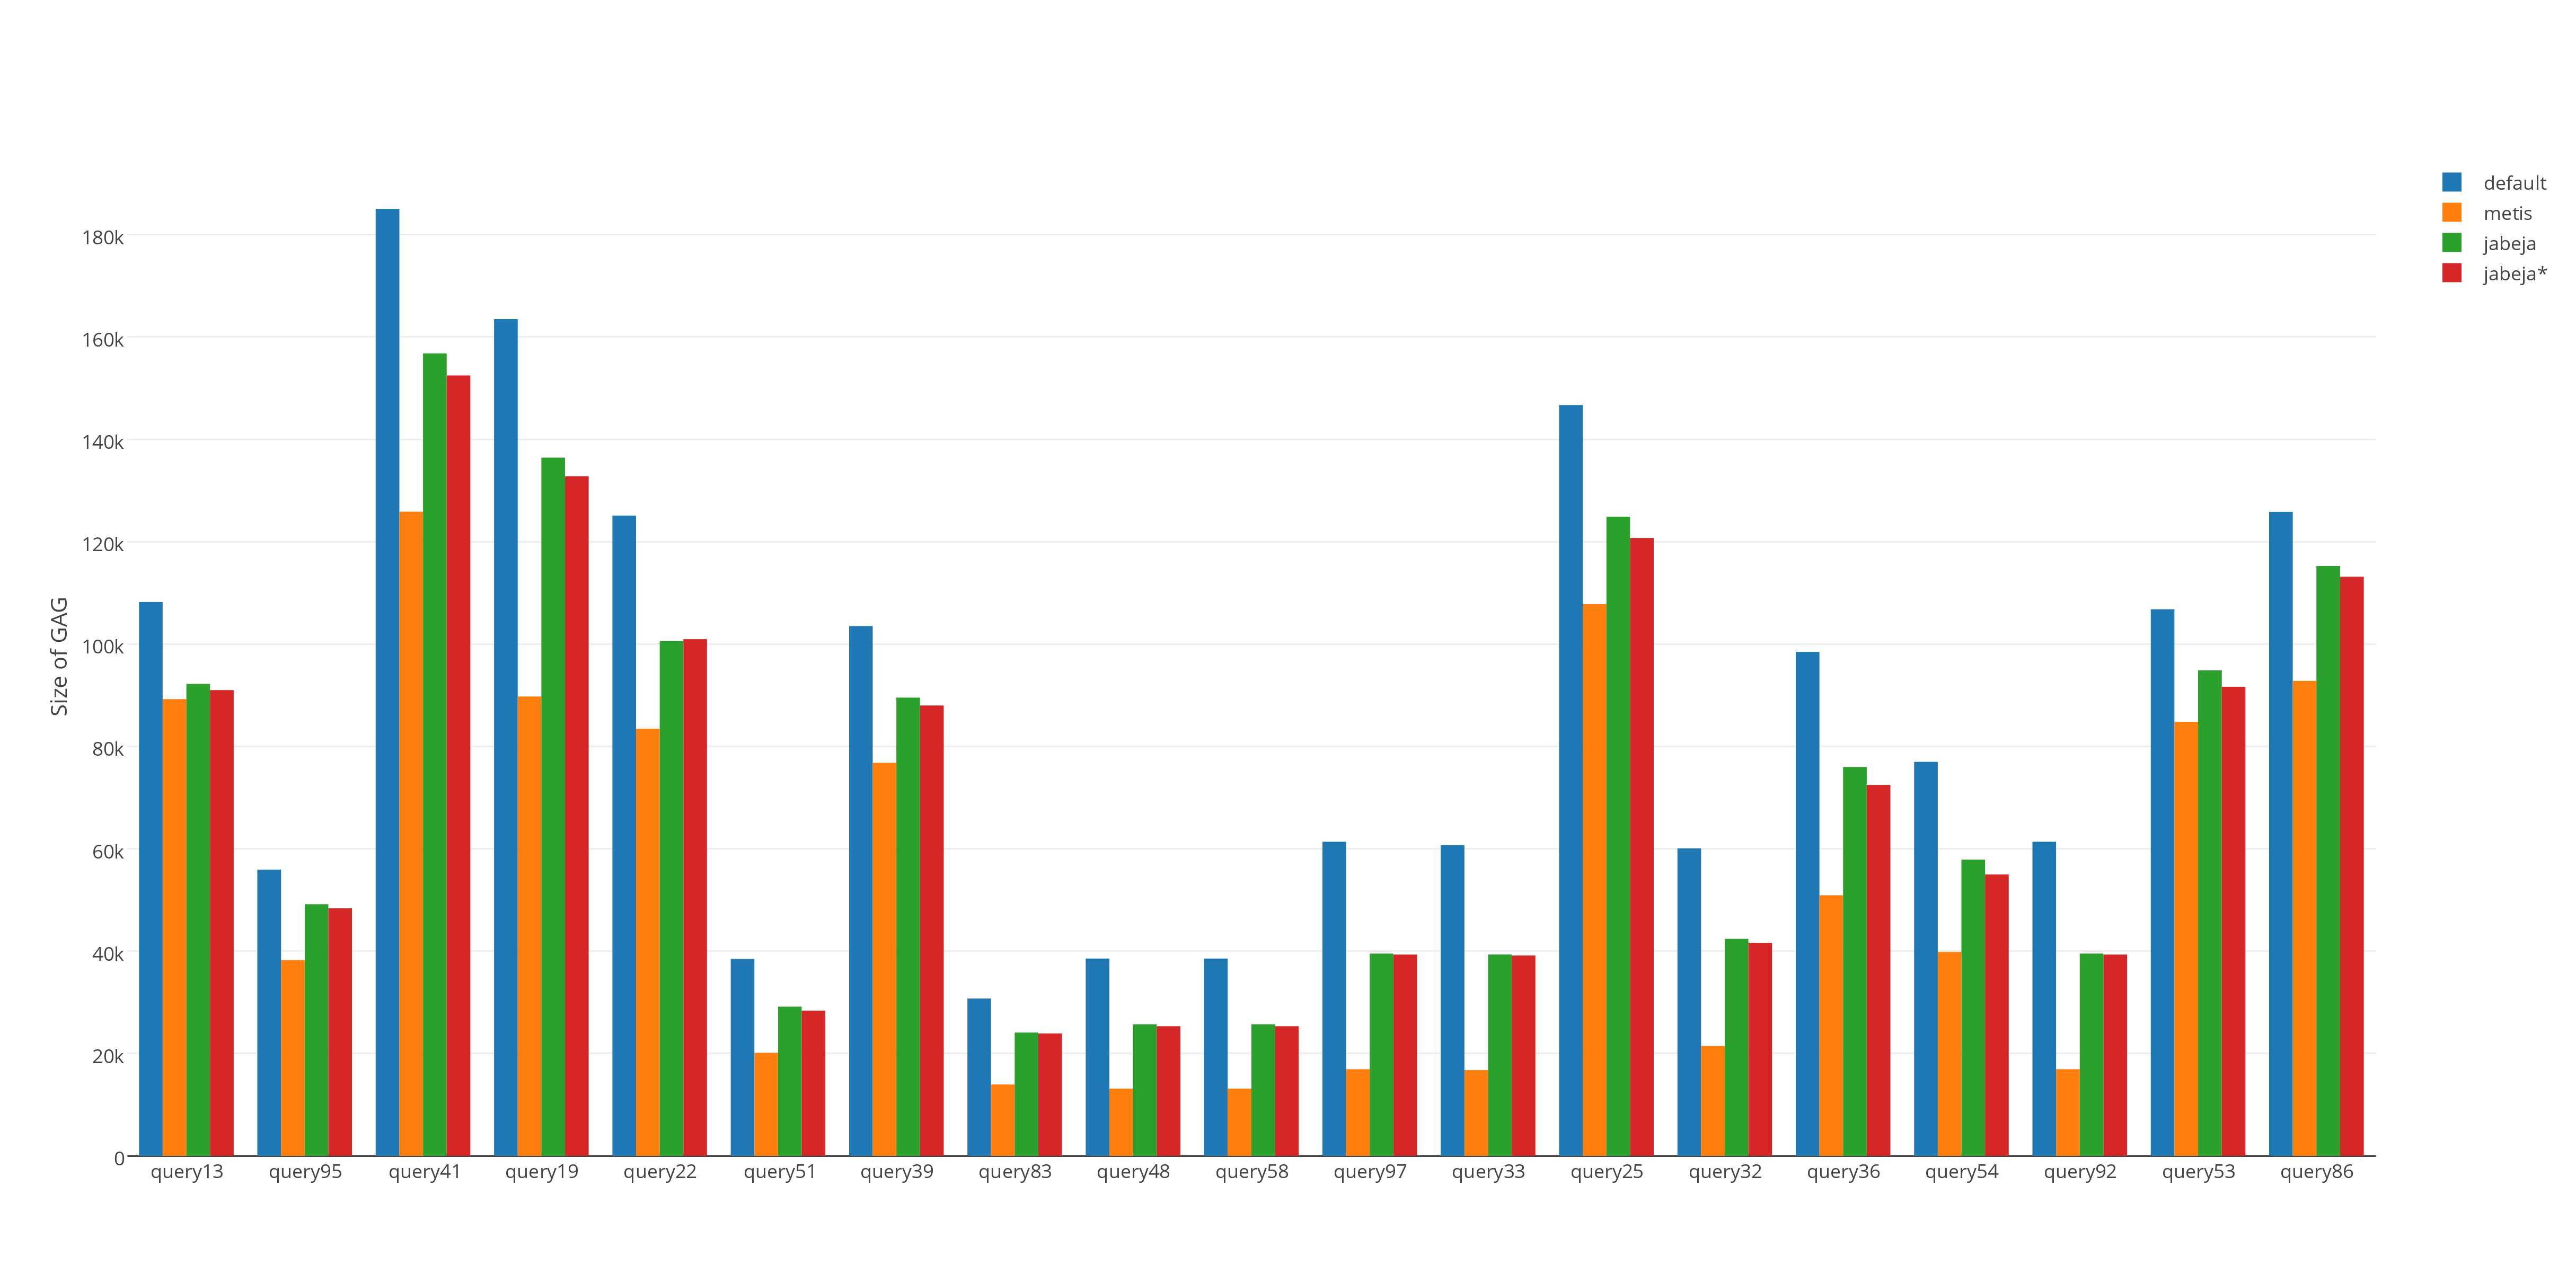
\includegraphics[width=1.0\textwidth]{img/gmark-01m-gag}
\end{figure}
\\The interesting findings are:
\begin{enumerate}
    \item The size of GAG is correlated with the number of input-nodes:
    \begin{enumerate}
        \item METIS has least input-nodes, which also leads to the small size of GAG.
        \item JABEJA* has fewer input-nodes and much more cross-edges than JabeJa, but it still produces the smaller size of GAG.
        \item Default partitioner is worst in GAG size, which is also consistent with the number of input-nodes.
    \end{enumerate} 
    \item The number of nodes in the GMark Graph doesn't influence the relevant results of different partition strategies since it's observed that all those three diagrams are in the same shape.
\end{enumerate}
\begin{figure}[h!]
  \caption{GAG size of GMark Graph ($10^6$ nodes)}
  \label{fig:gmark-1m-gag}
  \centering
    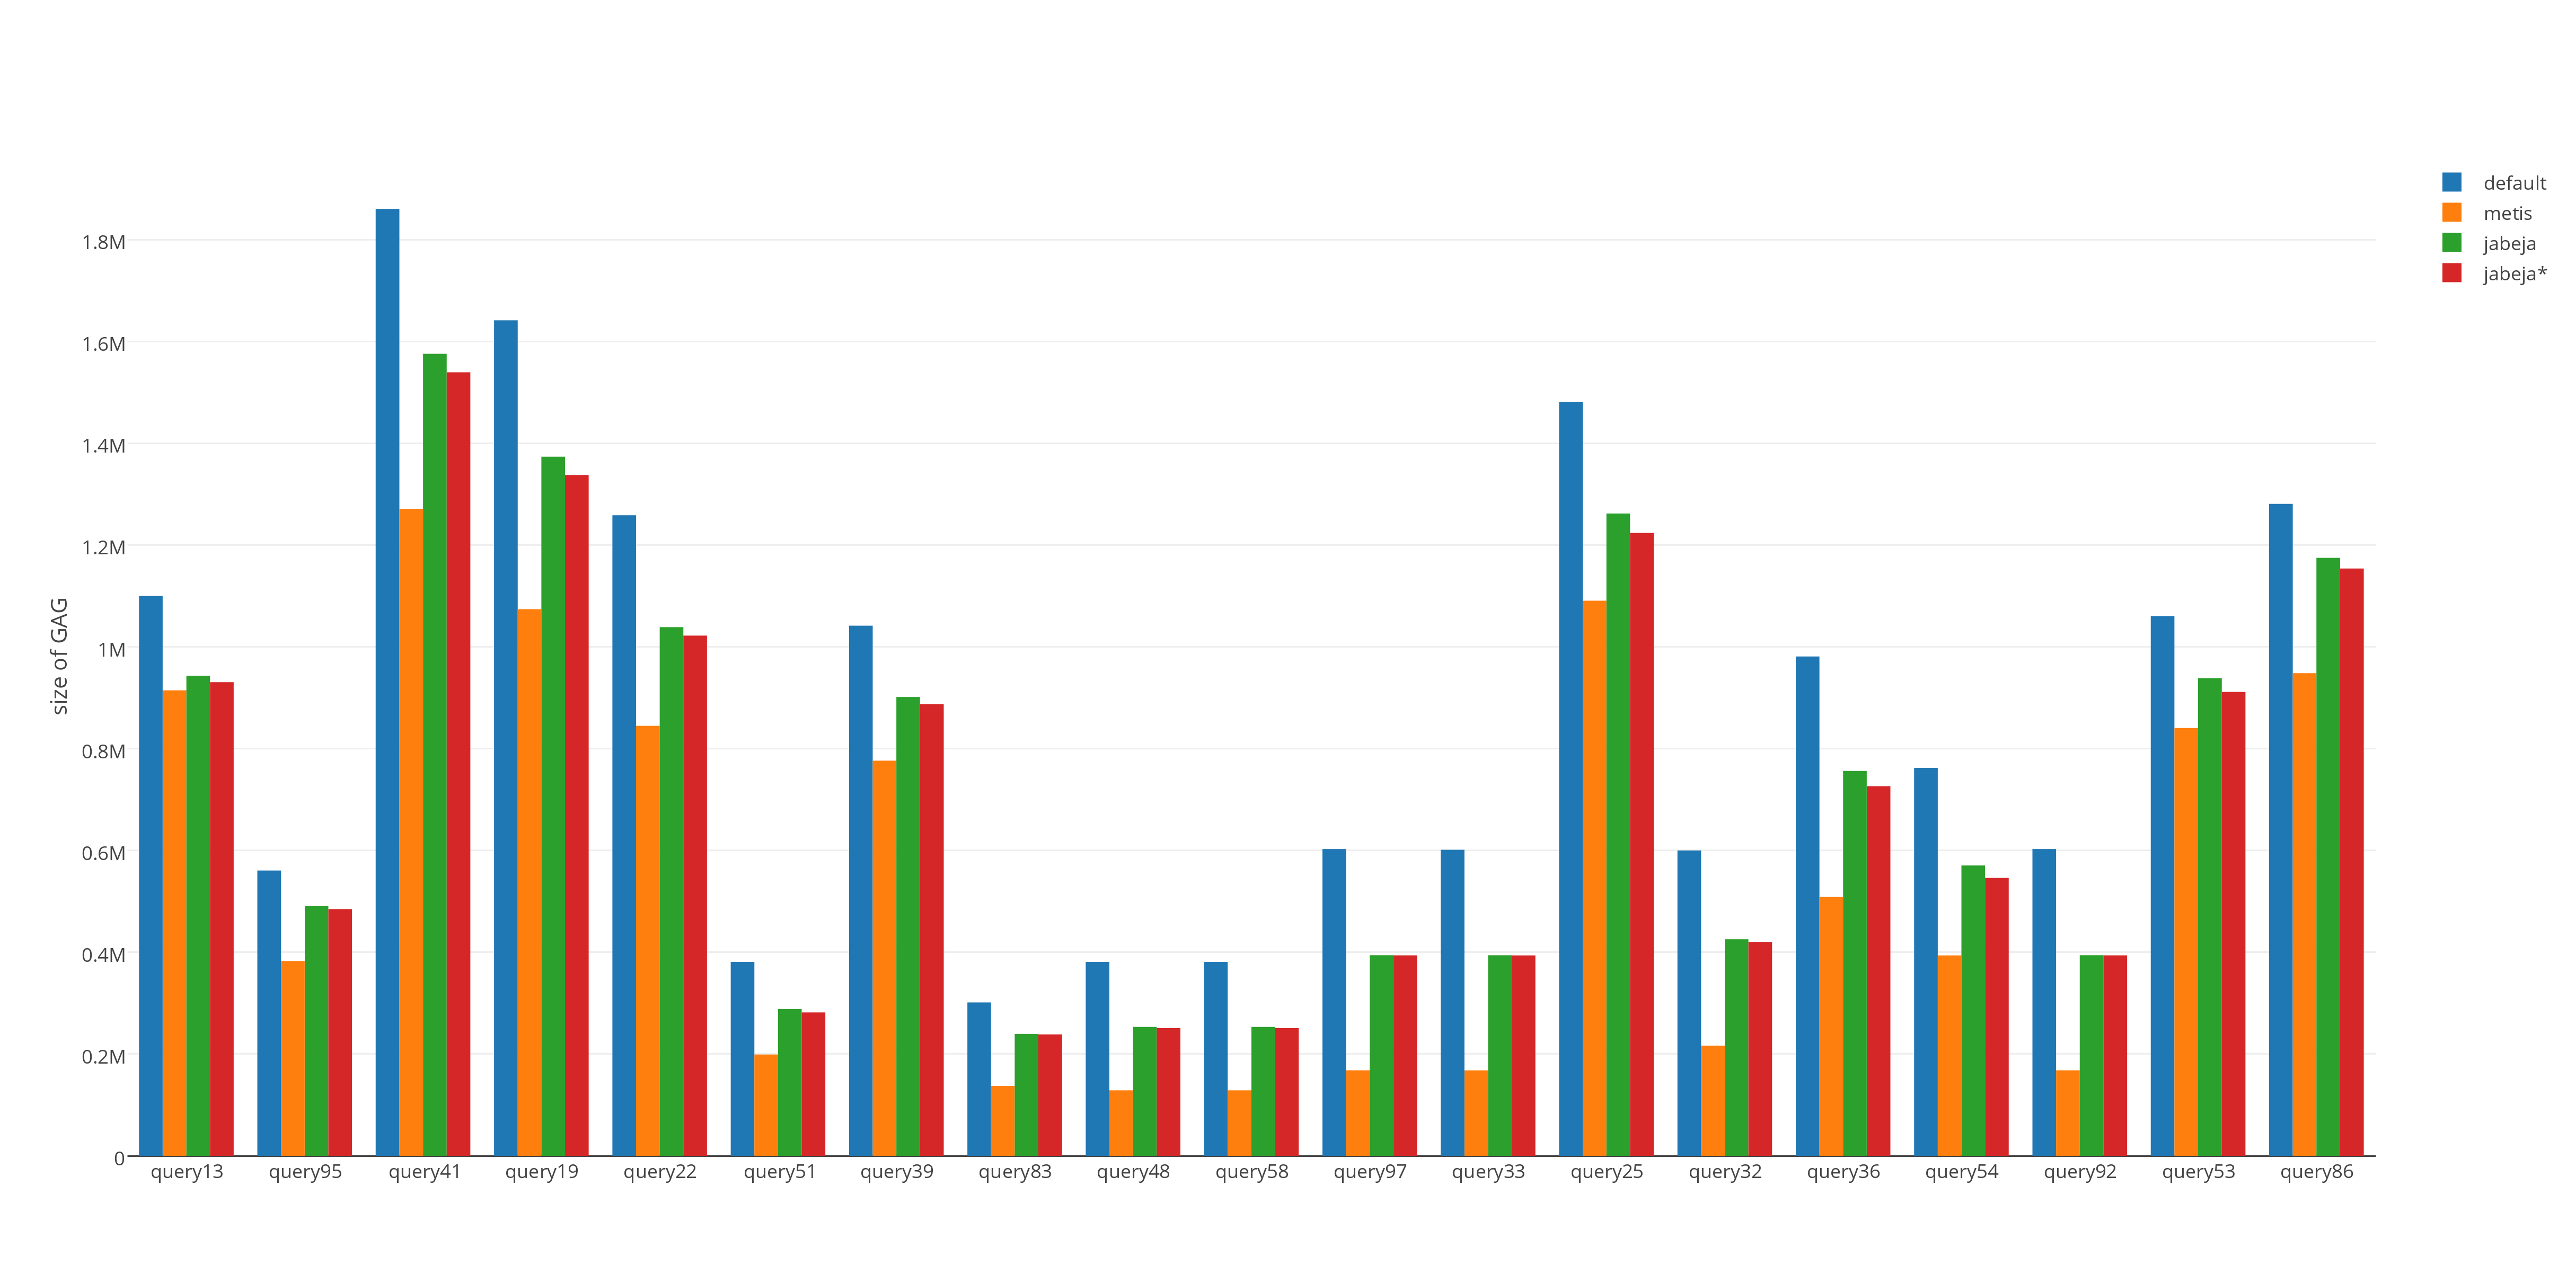
\includegraphics[width=1.0\textwidth]{img/gmark-1m-gag}
\end{figure}
\begin{figure}[h!]
  \caption{GAG size of GMark Graph ($10^7$ nodes)}
  \label{fig:gmark-10m-gag}
  \centering
    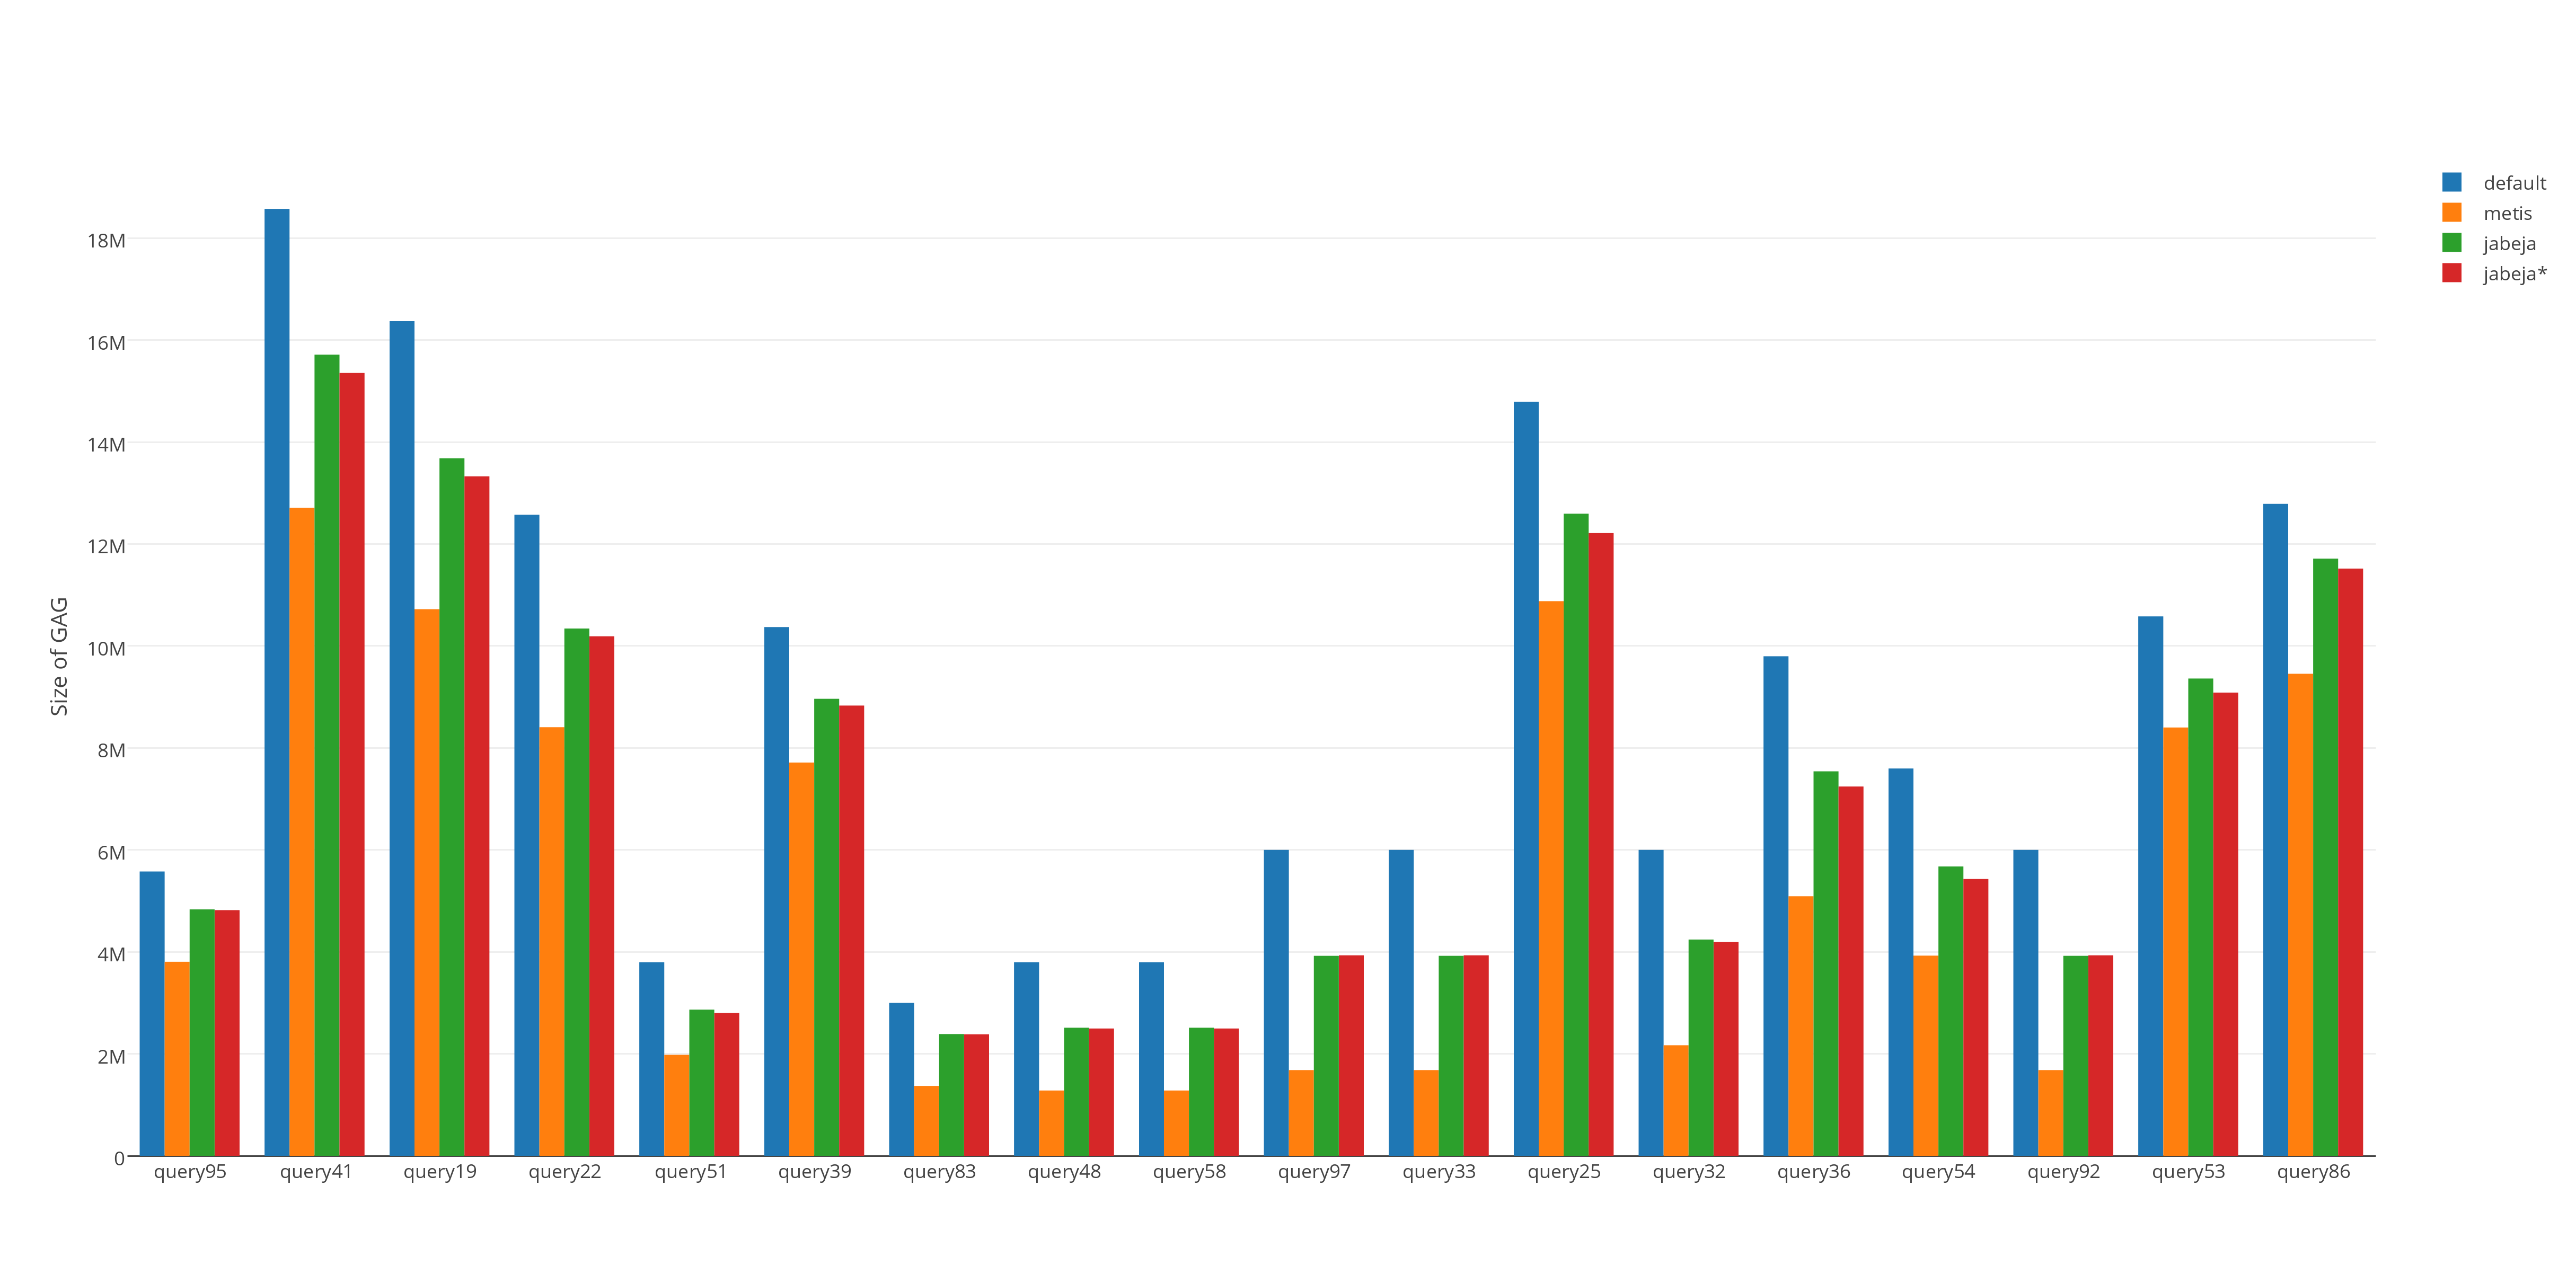
\includegraphics[width=1.0\textwidth]{img/gmark-10m-gag}
\end{figure}
We can see that in general METIS, JABEJA and JABEJA* are all improving the size of GAG to some extent. In the best case, the METIS could reduce the size of GAG to $30\%$, which could release the communication pressure during collecting GAG to driver significantly.

\subsection{Driver Computation Time}
Another reason of reducing the GAG size is that by pushing more work to executor side, the computation time on the driver side should be cut down accordingly. The time spent in the driver is described in Figure \ref{fig:gmark-01m-driver}, Figure \ref{fig:gmark-1m-driver} and Figure \ref{fig:gmark-10m-driver}. The x-axis is the index of queries in each benchmark and y-axis represents the time spent on the driver side in milliseconds.
\begin{figure}[h!]
  \caption{Driver Computation Time of GMark Graph ($10^5$ nodes)}
  \label{fig:gmark-01m-driver}
  \centering
    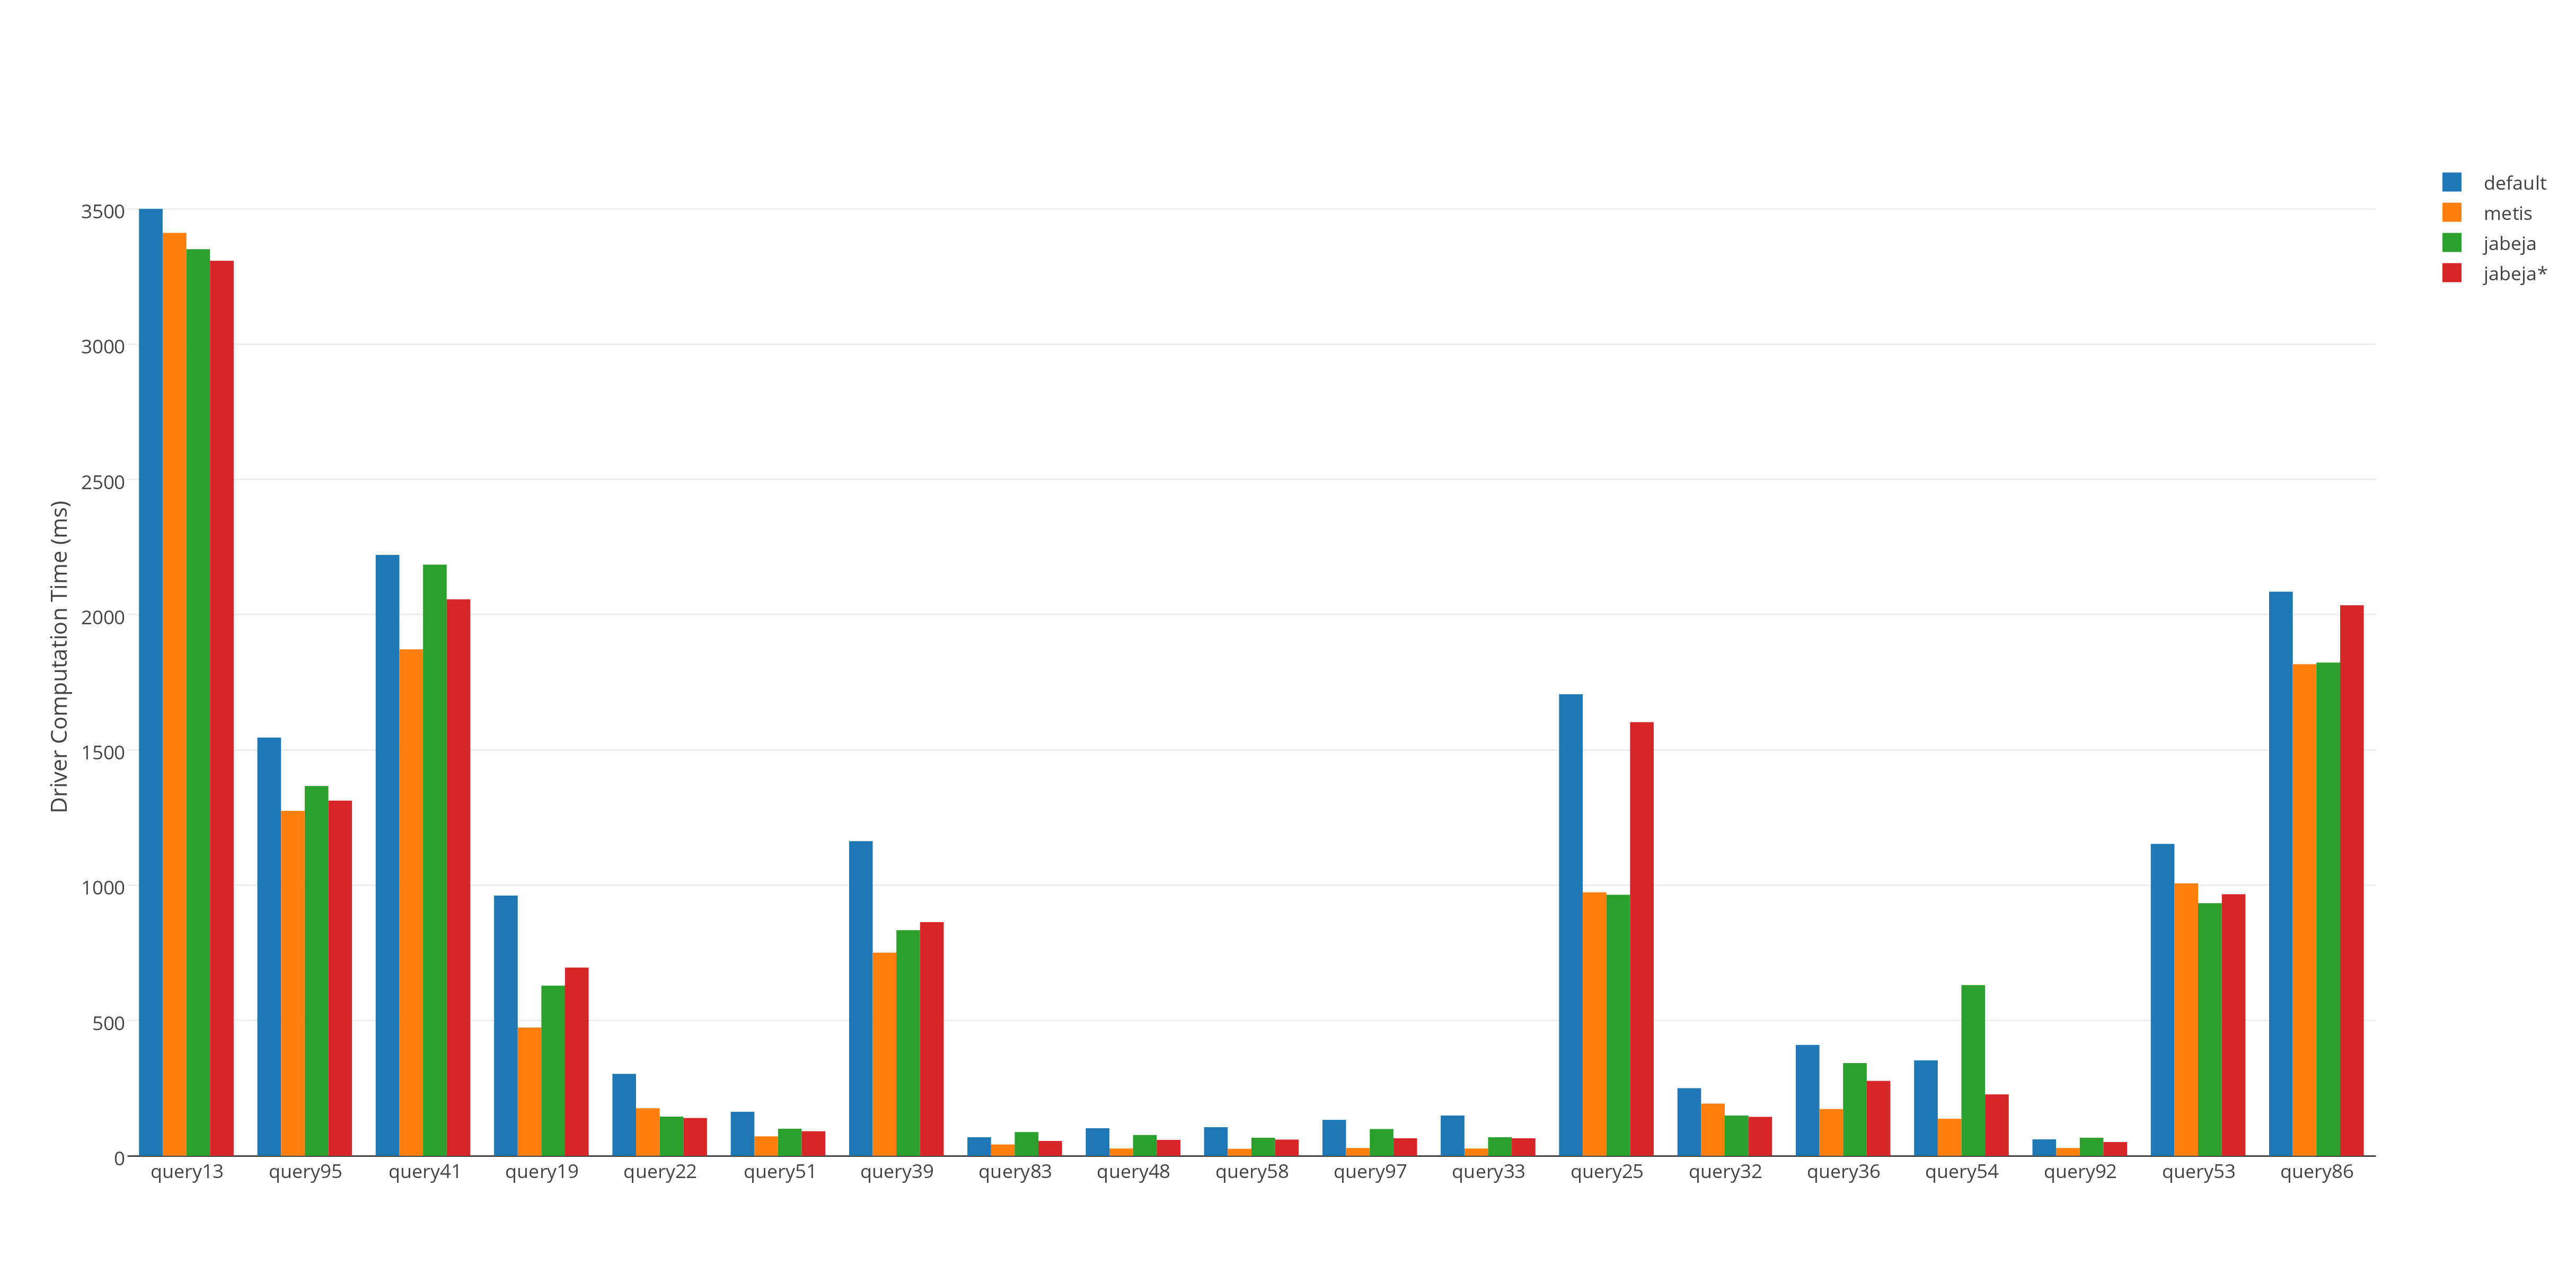
\includegraphics[width=1.0\textwidth]{img/gmark-01m-driver}
\end{figure}
\begin{figure}[h!]
  \caption{Driver Computation Time of GMark Graph ($10^6$ nodes)}
  \label{fig:gmark-1m-driver}
  \centering
    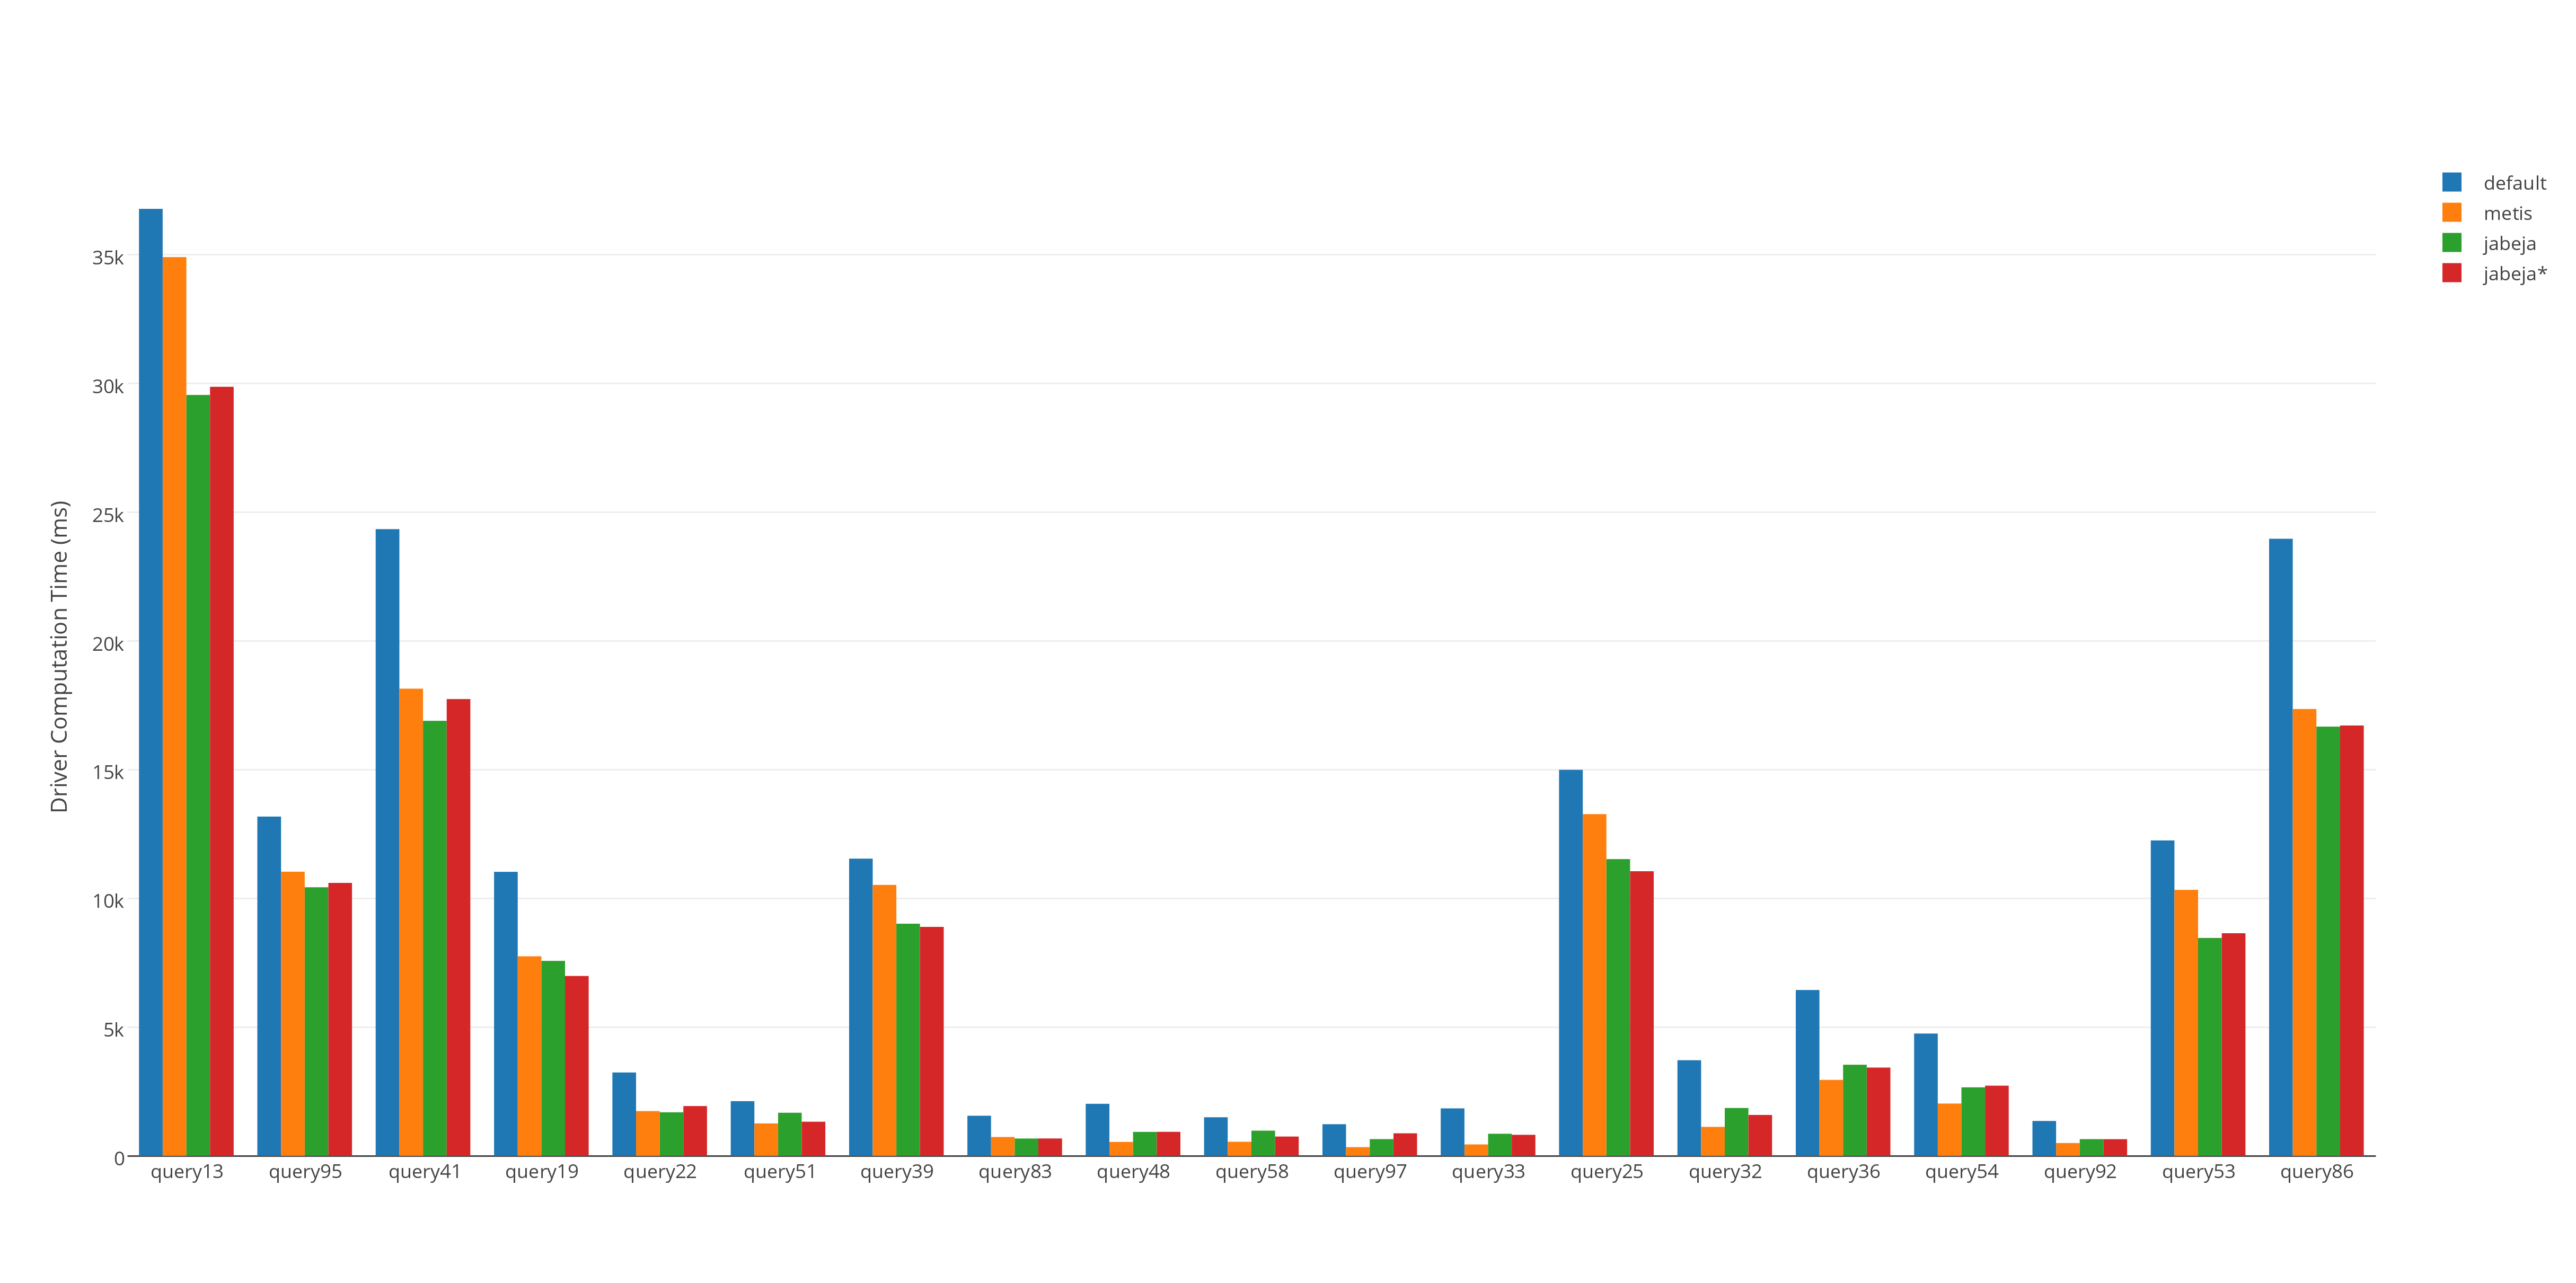
\includegraphics[width=1.0\textwidth]{img/gmark-1m-driver}
\end{figure}
\begin{figure}[h!]
  \caption{Driver Computation Time of GMark Graph ($10^7$ nodes)}
  \label{fig:gmark-10m-driver}
  \centering
    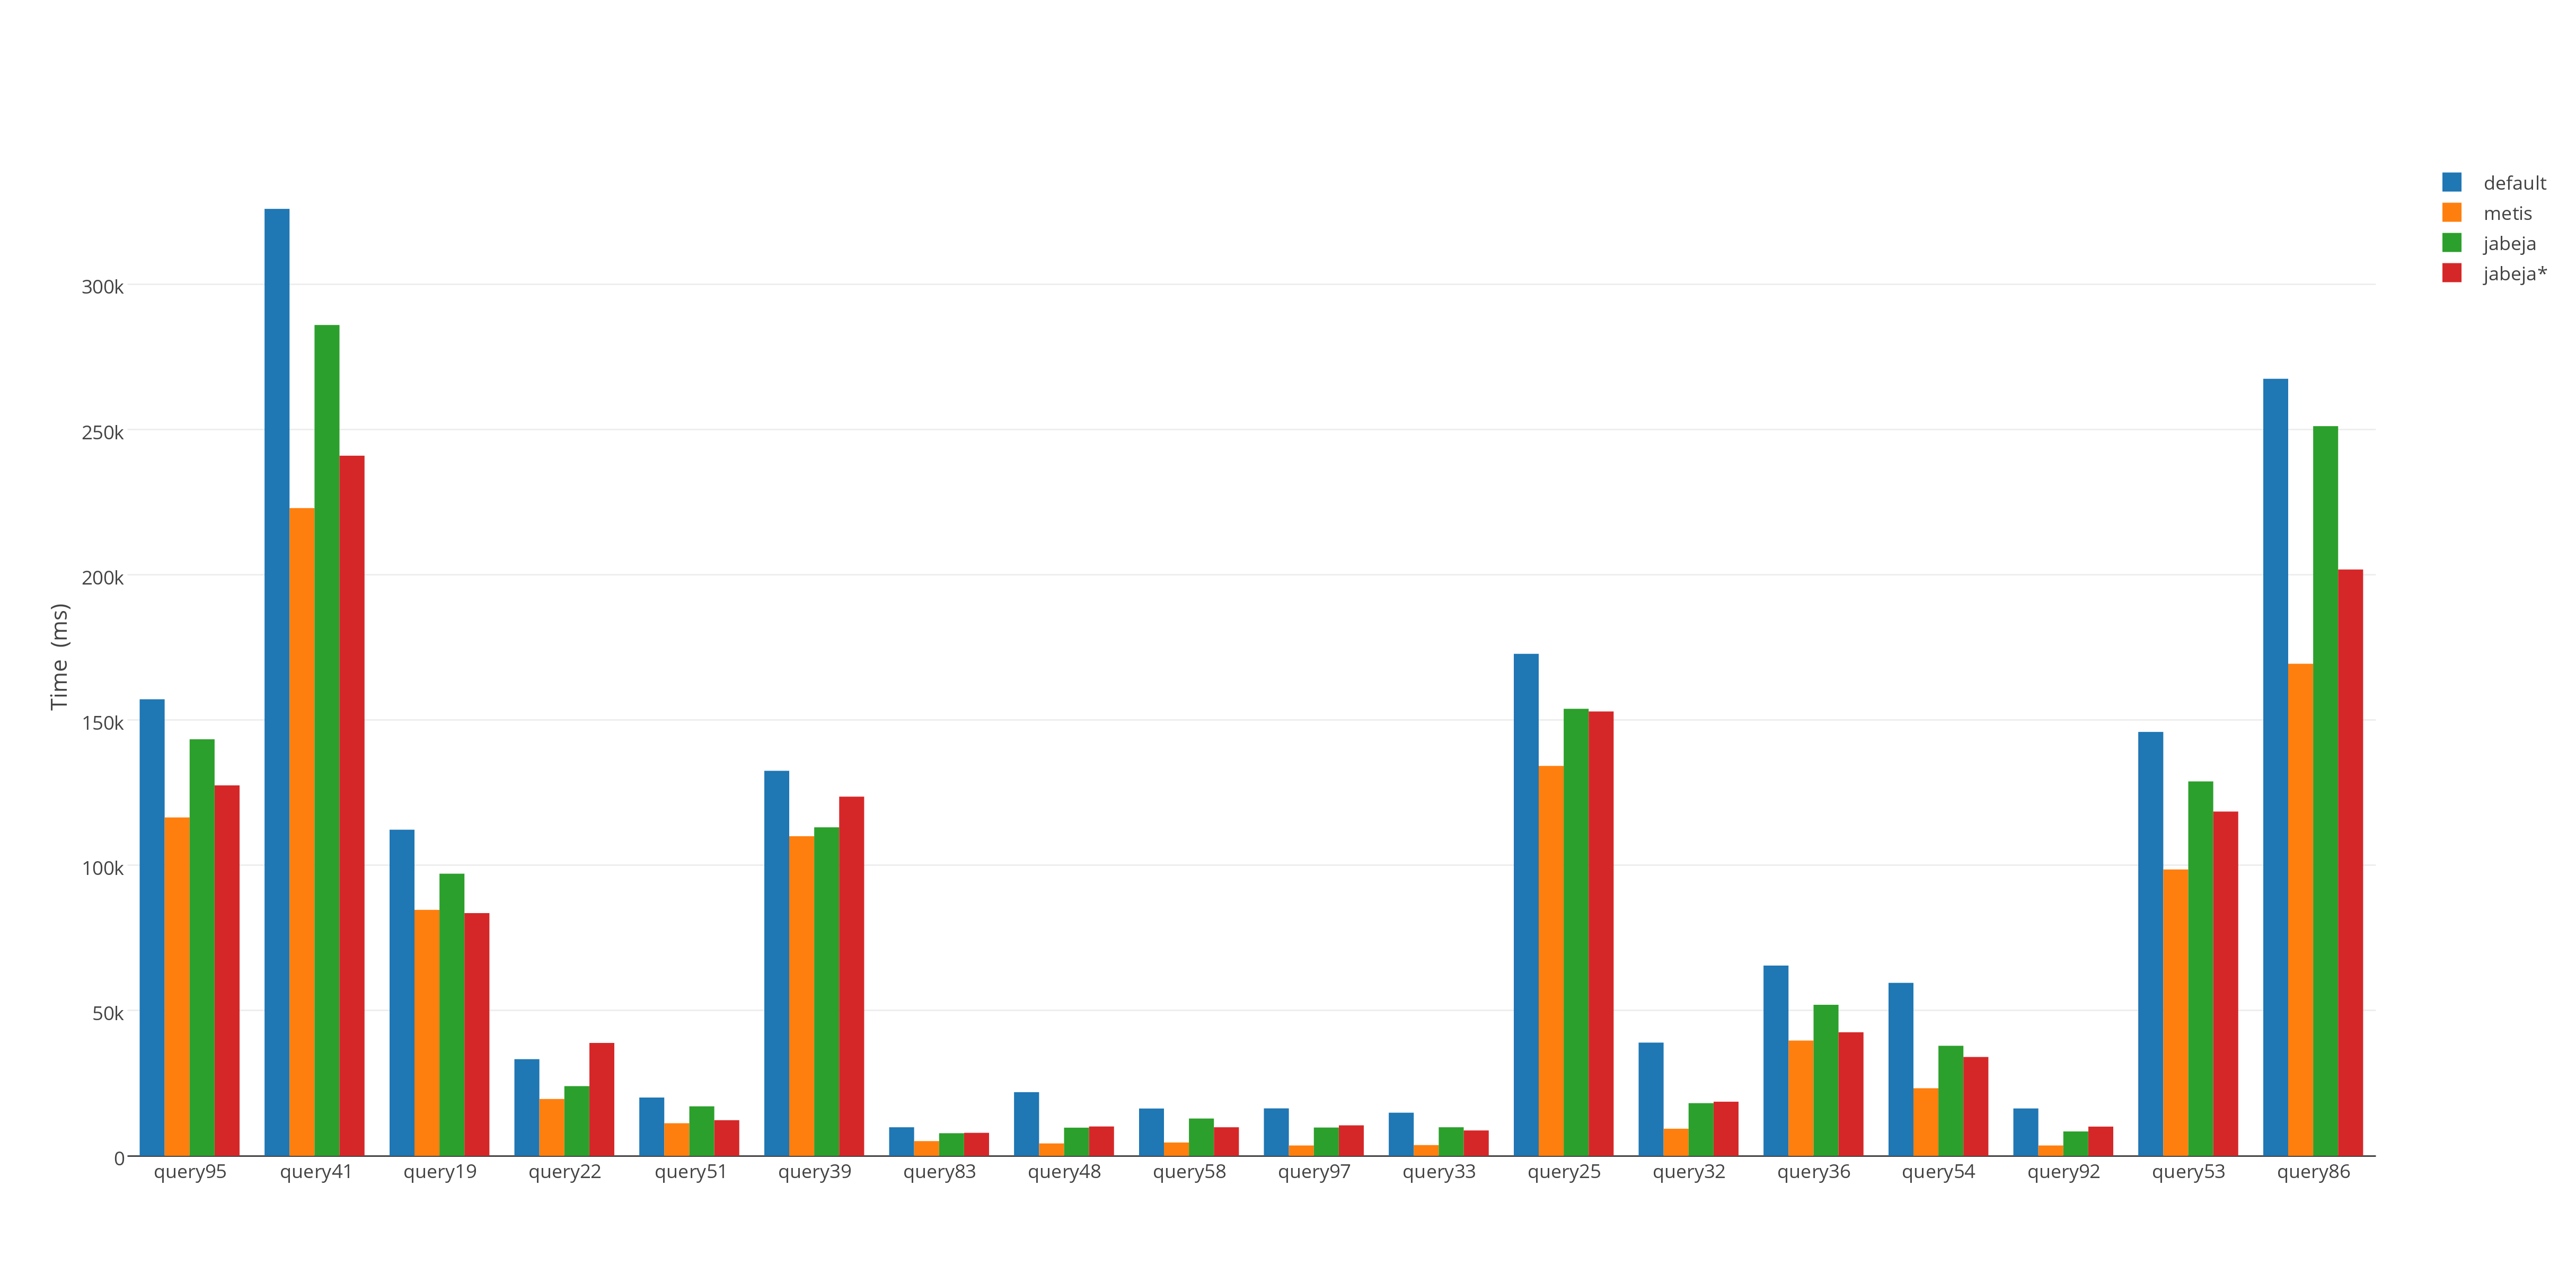
\includegraphics[width=1.0\textwidth]{img/gmark-10m-driver}
\end{figure}
The observations are:
\begin{enumerate}
    \item In most cases, the driver calculating time is consistent with the number of input-nodes and size of GAG.
    \item For some specific queries, such as query25 and query86 in Figure \ref{fig:gmark-01m-driver}, the JabeJa* takes more time than JabeJa. The reason behind is that although the size of GAG is similar, the computation time depends on the query itself and structure of GAG. Furthermore, the computation time only takes a few seconds, which means the reduced GAG size might not compensate the difference in the GAG structure. With increasing size of GAG, the special cases appear much less and when the nodes number is $10^7$, driver computation time of all queries are almost consistent with the trend of GAG size.
\end{enumerate}
\subsection{Overall Running Time}
Recall that in the Figure \ref{fig:alibaba-dan-jobs}, the driver computation can take more than $50\%$ percent of total time during evaluation. One of the goals of improving the partition strategies is to minimize the overall time. So besides the metrics we have already discussed above, we would like to investigate if the smart partition strategies are improving the total time spent on evaluation. The final result is list in Table \ref{overall-time}.
\begin{table}[h!]
\centering
\caption{Overall running time per query}
\label{overall-time}
\begin{tabular}{l|ll}
\hline
\#Nodes & strategy & time (ms)\\
\hline
\multirow{4}{*}{$10^5$}               & default & 95384  \\
                                      & METIS   & 74846  \\
                                      & JabeJa  & 86117  \\
                                      & JabeJa* & 76209  \\
\hline
\multirow{4}{*}{$10^6$}               & default & 43789  \\
                                      & METIS   & 63904  \\
                                      & JabeJa  & 58970  \\
                                      & JabeJa* & 69195  \\
\hline
\multirow{4}{*}{$10^7$}               & default & 505354 \\
                                      & METIS   & 562181 \\
                                      & JabeJa  & 289112 \\
                                      & JabeJa* & 404669 \\
\hline
\end{tabular}
\end{table}
According to the table, there are several key findings:
\begin{enumerate}
    \item The overall running time of size $10^5$ is consistent with the number of input-nodes or size of GAG. There are several queries which have driver-side bottleneck and are improved significantly.
    \item The overall running time of size $10^6$ is completely in contrast to the trend in the number of input-nodes. This is because we remove the queries with driver-side bottleneck as they take too much time to evaluate sequentially, and the rest of queries don't have such bottleneck (The time spent on the driver side is less than $10\%$ for all the queries). Then, compared  to the few seconds ahead on driver side, the overhead brought by more iterations in the distributed system is the dominant factor.
    \item The overall running time for size $10^7$ is in between the previous two situations: There are no queries which invest more than $90\%$ time on driver side, but the average proportion of time spent on driver still increases compared to the graph of $10^6$ nodes.
\end{enumerate}
In Table \ref{driver-queries}, we list several queries that have the driver-side bottleneck. It could be observed that the larger ratio driver time has, the bigger improvement in overall time could partition-strategies achieve.
\begin{table}[] \small
\centering
\caption{Durations for Queries having Driver-side Bottleneck in ms}
\label{driver-queries}
\begin{tabular}{l|ll|ll|ll|ll|}
        & \multicolumn{2}{c|}{default} & \multicolumn{2}{c|}{METIS} & \multicolumn{2}{c|}{JabeJa} & \multicolumn{2}{c|}{JabeJa*} \\ \cline{2-9} 
        & driver        & overall      & driver      & overall      & driver       & overall      & driver       & overall       \\ \hline
query79 & 1131742       & 1184438      & 583344      & 684098       & 723931       & 774945       & 743393       & 797520        \\
query95 & 157175        & 467259       & 116484      & 395386       & 143382       & 311311       & 127518       & 411474        \\
query41 & 325978        & 1203186      & 222985      & 901448       & 285998       & 682628       & 241008       & 678135        \\
query19 & 112272        & 890674       & 84667       & 706296       & 97117        & 414311       & 83557        & 554804       
\end{tabular}
\end{table}
\subsection{Answers for Research Questions}
\subsubsection{Research Question 1}
In most cases JabeJa* performs better than JabeJa but still worse than METIS. The reason behind this might be the choice of parameters: the algorithm finds 5 random nodes when there is no optimal neighbor to swap color.  The number might be still too small in the large graph, and put the program into a local optimum. In some quick tests, increasing this parameter to 30 can improve the quality significantly. However, as the implementation is sequential and only simulates the result, it takes too long to run with such random nodes.  Besides, we do not use any sampling policies such as in \cite{awan2006distributed} and \cite{dowling2012shuffling}. 
\subsubsection{Research Question 2}
The size of GAG decreases for different benchmarks, and for each benchmark in various sizes with the decreasing number of input-nodes. In all cases, reducing the number of input-nodes can formulate a better structure for graph and lessen the quantity of GAG states collected to the driver.
\subsubsection{Research Question 3}
In most cases, the declining size of GAG can result in less time spent on the driver, but when the GAG sizes are close, the computation time may depend on the structure of GAG and query itself.
\subsubsection{Research Question 4}
The speedup in overall time depends on the proportion of time spent on the driver. For those queries with driver-side bottleneck, reducing GAG size can lead to significant decrease in overall running time.
\section{Summary}
In this chapter, we firstly look into the reasons for the bottleneck on driver side when running Dan Suciu's Algorithm. Based on the idea that smart partition strategies can optimize the performance, we looked into the relationships between different metrics such as the number of input-nodes, the size of GAG and running time. The existing partition strategies and one modified strategy are clustered and tested against multiple benchmarks. Based on final results of the experiments, smart partition-strategies can optimize the size of GAG, the data collected in the network and the driver performance significantly by reducing the input-node size. %\chapter{\label{cha:vs-tree}Vertex Signature Tree in CRPQ Evaluation} 

\chapter{\label{cha:conclusions}Conclusions and Future Work}

This chapter firstly gives the contributions of the thesis work. Then the conclusion will be discussed concerning research questions. In section 9.3 we will go through the limitation of the project and provide possible improvement direction in Future work.

\section{Contributions}
The contributions of the project can be summarized as three parts:
\begin{enumerate}
    \item We give detailed data model and system architecture to store and evaluate regular path queries with Apache Spark and distributed storage back-ends.
    \item We customize three algorithms to return pairs of results for regular path queries. Specifically for the Multi-way Join, we deducted the formulas to evaluate regular path query with different situations such as with recurrence and shared variable less than 1. For all algorithms, time complexity and cost expression are analyzed carefully. We point out possible bottlenecks for those algorithms and the data supporting them.
    \item We optimize the performance of Dan Suciu's algorithm with different partition strategies. The policies cover different approaches such as multi-level partitioning or 'gossip' way. We give a more general cost expression comparing to Dan Suciu's model.
\end{enumerate}

\section{Conjectures}
In the evaluation chapter, the cascaded two-way join turns out to be the most scalable algorithm since tasks are evenly distributed, and there is no computation on driver side, although the algorithm conducts frequent full shuffles. The multi-way join shuffles less in most cases while the performance gets worse rapidly with the introduction of recurrence. Dan Suciu's Algorithm makes use of the data locality and seldom does shuffling.

\section{Conclusions}
For modified Dan Suciu's Algorithm, the computation on the driver side is the bottleneck and cannot handle real huge GAG. In chapter 8, we propose a cost expression that is more accurate to describe network volume comparing to Dan Suciu's model. In the best case, the optimization by METIS strategy reduces the communication size to $30\%$ and overall running time to $50\%$.

\section{Limitations and Future work}
One limitation of this thesis work is the simple selection of parameters for multiple algorithms:
\begin{enumerate}
    \item In multi-way join, we only tested with $k=128$. The running time and shuffle size may vary with different $k$.
    \item In JabeJa* only one set of parameters initial temperature $T_0$ and cool down speed $\theta$ for simulated annealing is applied. Changing these parameters can relax or restrict the swap conditions in each iteration, which could potentially have huge impact on the final result.
    \item In JabeJa* we only check five random nodes once there is no suitable neighbor, which might influence the partition quality.
    \item In GMark benchmark, we only generate graphs with one set of parameters, which means the graphs are in similar shape. The algorithms can be evaluated on more benchmarks with variability.
\end{enumerate}
Furthermore, the JabeJa* algorithm is only implemented sequentially and simulate the result. One future research could focus on the asynchronous implementation in GraphChi and discuss the rounds needed for convergence.
\\Besides, the partition strategies can only optimize for those queries with "light" head. For other kinds of queries, other techniques such as indexes could be used for optimization.
\\The driver side hangs when the GAG size is of thousands of millions, which means the complex queries on a large graph may be unsolvable for Dan Suciu's Algorithm. One topic for future work is to distribute GAG to cluster again and discuss optimization techniques for the computation.
\\We only examined the influence of different partition strategies on Dan Suciu's Algorithm. Although the Cascaded 2-way Join and the Multi-way Join only do full shuffles which are irrelevant to partition strategies, it would be interesting to explore if the smart partition algorithms could reduce remote communication and keep shuffling on local nodes as much as possible.

\bibliographystyle{plain} \bibliographystyle{plain}
\bibliography{thesis}


\appendix
%dummy comment inserted by tex2lyx to ensure that this paragraph is not empty
\global\long\def\chaptername{Appendix}
 
\chapter{\label{cha:glossary}Queries}

\section{Alibaba}
\subsection{Real-World Queries}
Query 1: C+ "acetylation" A+
\\([7]|[28]|[8]|[13]|[45]|[68]|[38])+ [143] \\([3]|[4]|[11]|[15]|[19]|[21]|[43]|[22]|[32]|[96])+
\\Query 2: C+ "acetylation" I+
\\([7]|[28]|[8]|[13]|[45]|[68]|[38])+ [143] \\([24]|[60]|[29]|[34]|[9]|[6])+
\\Query 3: C+ "methylation" A+
\\([7]|[28]|[8]|[13]|[45]|[68]|[38])+ [202] \\([3]|[4]|[11]|[15]|[19]|[21]|[43]|[22]|[32]|[96])+
\\Query 4: C+ "methylation" I+ 
\\([7]|[28]|[8]|[13]|[45]|[68]|[38])+ [202] \\([24]|[60]|[29]|[34]|[9]|[6])+
\\Query 5: C+ "fusions" P
\\([7]|[28]|[8]|[13]|[45]|[68]|[38])+ [446] \\([272]|[273]|[480]|[479]|[111]|[199]|[157]|[5])
\\Query 6: "fusions" A+ 
\\\relax [446] ([3]|[4]|[11]|[15]|[19]|[21]|[43]|[22]|[32]|[96])+
\\Query 7: A+ "receptor" P 
\\([3]|[4]|[11]|[15]|[19]|[21]|[43]|[22]|[32]|[96])+ [153] ([272]|[273]|[480]|[479]|[111]|[199]|[157]|[5])
\\Query 8: I+ "receptor" P
\\([24]|[60]|[29]|[34]|[9]|[6])+ [153] ([272]|[273]|[480]|[479]|[111]|[199]|[157]|[5])
\\Query 9: A A+
\\([3]|[4]|[11]|[15]|[19]|[21]|[22]|[32]|[96]) ([3]|[4]|[11]|[15]|[19]|[21]|[22]|[32]|[96])+
\\Query 10: I I+
\\([24]|[29]|[34]|[9]|[6]) ([24]|[29]|[34]|[9]|[6])+
\\Query 11: C E
\\([13]|[8]|[7]) ([2]|[19]|[21]|[23]|[17])
\\Query 12: A+ I+
\\([3]|[4]|[11]|[15]|[19]|[21]|[22]|[32]|[96])+ ([24]|[29]|[34]|[9]|[6])+
\subsection{"Light Head" Queries}
Query 16: [243]+[1]
\\Query 17: [1][1]+[25]
\\Query 18: [49][361][1]+
\\Query 19: [21]+[455][1]
\\Query 20: [65][291][1]\*
\\Query 21: [17]+[315][1]+
\\Query 22: [15]+[610][1]+
\\Query 23: [2]+[566]
\subsection{Random Queries}
[0]\*([1]+[0][0])
\\([0][0][0])+[0]\*
\\\relax [0][0][0][1]\*[0]+[1]
\\\relax [0][0]+[2][0]\*[1]+[0]\*[1]\*
\\\relax [1]\*[0]+
\\\relax [1][0]\*[1]+[0]+([0]\*[1][1]\*)\*([0][0][0][0])[4]
\\\relax [0][0]\*[1][0]+
\\\relax [0][0]\*[1]+
\\\relax [0][1][0][0]\*[1]+[0]+[1]+[0][0]
\\\relax [1]+[0]([0][0][0])\*[0]\*[45]
\\\relax [0][0][0]([1][0][0][1][0]+)[0][0]\*
\\([0]+[1]+[25])+[0][0]\*
\\\relax [0]+[1]+[0]\*[1][0]\*[1]\*
\\\relax [0]+[1]+[0]+([0]\*[1][0][0])
\\\relax [1][0][0][0]\*[260]+[0]+
\\\relax [1][0]\*[1]+[0][0][0]
\\\relax [0][0]\*[1][0]+[1]\*[0][0]
\\\relax [0][0][1]\*[0]\*[1]+[0]+
\\\relax [1]\*[0][1]+[0]
\\(([0]\*[2][0])[1]\*[0][1])\*[0][0]+[1][1]
\\\relax [0]\*[1]\*[0]\*[1]+
\\\relax [1][0][1]\*[0][0]+[1]
\\\relax [0][0]\*[1]+[0]+
\\\relax [1][0][0]\*[1]+
\\\relax [0]+[1][0][0]\*[1][0]
\\\relax [1][0]\*[1]+[0][1]
\\\relax [56]\*[0][1]+
\\([1][0][1])([1][0][0]+[1])+([0][0][0][0])\*[0]+[1]
\\\relax [0][0][0]\*[1]+
\\\relax [0][0]\*[130]+[0][0]
\section{GMark Graph}
Query 13: ([1-][0-][0])|([1-][0-][0])|([1-][0-][0])
\\Query 19: ([3-][3][3-][0-])|([3-][1][1-][0-])
\\Query 22: ([2-][1-][3][3-])|([2-][1-][0-][0])|([2-][1-][3][3-])
\\Query 25: ([3-][1][1-])|([3-][0-][0])
\\Query 32: ([1-][1][2])
\\Query 33: (([2-][1-][1][2])|([2-][1-][1][2]))*
\\Query 36: ([3-][1][1-][1])
\\Query 39: ([3-][3][3-])|([3-][0-][0])
\\Query 41: ([1-][3][3-][0-])|([1-][1][1-][0-])
\\Query 48: ([3-][1][2])|([3-][1][2])
\\Query 51: ([1-][3])|([1-][3])
\\Query 53: ([1-][1][1-])|([1-][3][3-])
\\Query 54: ([3-][1][1-][3])
\\Query 58: ([3-][1][2])|([3-][1][2])
\\Query 72: (([3-][3])|([3-][1][1-][3])|([3-][3][3-][3]))*
\\Query 79: (([3-][0-][0][3])|([3-][1][1-][3])|([3-][3]))*
\\Query 83: ([1][2])|([1][2][2-][2])
\\Query 86: ([3-][0-])|([3-][0-][0][0-])|([3-][0-])
\\Query 92: (([2-][1-][1][2])|([2-][2]))*
\\Query 95: (([2][2-]))*
\\Query 97: (([2-][1-][1][2])|([2-][1-][1][2])|([2-][2]))* \include{requirements}
\end{document}
